%------------ Hinweise --------------------------------------------
% Um das fertige Dokument zu erstellen, wie folgt vorgehen:
% 1. pdflatex Diplomarbeit.tex
% 2. makeindex Diplomarbeit.idx -s Diplomarbeits.ist -t Diplomarbeit.nlg -o Diplomarbeit.nls 
% (Alternativ sollte auch makeindex Diplomarbeit funktionieren)
% 3. makeglossaries Diplomarbeit
% 4. biber Diplomarbeit
% 5. pdflatex Diplomarbeit.tex
%
% Das ganze lässt sich in diversen Editoren (z.B. TeXnicCenter) in fertigen Profilen 
% speicheren bzw. durch leichte Abwandlung schon vorhandener Profile erreichen. Beim
% allerersten Aufruf ist der ganze Ablauf zweimal nötig, um alle Referenzen usw.
% aufzulösen!
%
% Die hier geladenene Pakete stellen viele grundlegende Funktionen zur Verfügung. 
% Alles weitere bitte selbst hinzufügen.


%------------ Header --------------------------------------------
\documentclass[%
  ngerman,%
  BCOR=0mm,
  cdgeometry=yes,
  numbers=noenddot,
  paper=a4,
  listof=totoc, bibliography=totoc,
]{tudscrreprt}
\iftutex
  \usepackage{fontspec}
\else
  \usepackage[T1]{fontenc}
  \usepackage[ngerman=ngerman-x-latest]{hyphsubst}
\fi
\setcounter{secnumdepth}{4} % Ueberschriften bis 4. Ebene nummeriert
\setcounter{tocdepth}{4} 		% Ueberschriften bis 4. Ebene in Inhaltsverzeichnis


%------------ Deutsche Anpassungen und Schrift ------------------------------------
\usepackage[ngerman]{babel}
\usepackage[style=numeric, backend=biber]{biblatex}
\usepackage[T1]{fontenc}			 % Font-Encoding, welches Umlaute unterstützt
\usepackage[utf8]{inputenc} % Tex-Dateien werden ANSI-Kodiert erwartet. Umlaute können direkt im Tex-Dokument verwendet werden
\usepackage{textcomp}
\usepackage{gensymb}

\usepackage{csquotes}		% Für biblatex
\usepackage{lmodern}     			 % Umfangreiche und hübsche Schriftart

\usepackage{caption}    			 % Captions außerhalb von floats erstellen
\usepackage{upgreek}		 			 % Grichische Einheiten nicht kursiv darstellen

% \usepackage[default]{opensans}
\usepackage[ngerman]{babel}							% Deutsche Bezeichner
\addto\captionsngerman{%								% Macht aus der Beschriftung Abbildung --> Abb.
	\renewcommand{\figurename}{Abb.}%			%
	\renewcommand{\tablename}{Tab.}%			%
}
  

%------------ Grafiken und Abbildungen --------------------------------------------
\usepackage[pdftex]{graphicx} % Grafiken in pdfLaTeX
\usepackage{float}						% Das Bild mit [ht] wenn möglich an der Stelle wie im Tex-Dokument ausgeben.
\pdfinclusioncopyfonts=1 			% Richtige Darstellung der in Matlab erstellten Axenbeschriftungen

\usepackage{subcaption}				% Mehrere Bilder in einer Figure Umgebung mit separaten Bildunterschriften

\renewcommand{\thefigure}{\arabic{chapter}.\arabic{figure}}		% Abbildungsnummerierung im Format Kapitel.Nummer


%------------ Formeldarstellung --------------------------------------------
\usepackage{amsmath}     % Mathematische Befehle
\usepackage{amssymb}     % Erweiterte math. Symbole lädt implizit amsfonts
\usepackage{amstext}		 % \text{} im math-modus
\usepackage{siunitx}		 % Korrektes Verwendung von Einheiten mit \SI{Zahl}{\einheit}


%------------ Zeilenabstand und Absätze --------------------------------------------
\usepackage{setspace}		% Zeilenabstand einstellen
%\singlespacing					% 1-zeilig (Standard)
\onehalfspacing					% 1,5-zeilig
%\doublespacing					% 2-zeilig

\setlength{\parindent}{1em}	% Einrücktiefe von neuen Absätzen


%------------ Seitenlayout --------------------------------------------
\usepackage{geometry}                % Ändern der Seitengeometrie. 
\usepackage{pdflscape}

%------------ Header und Footer --------------------------------------------
% Fuß- und Kopfseparierungslinie im scrlayer style. Im plain.scrlayer style nur eine Fußlinie
\usepackage[headsepline=0.5pt,footsepline=0.5pt,plainfootsepline]{scrlayer-scrpage}

\KOMAoptions{onpsinit=\setstretch{1.2}} % Verhindert die Beeinflussung von header und footer durch spacing Umgebungen
% \pagestyle{scrheadings}

\ohead{\leftmark}		% Kapitel außen in der Kopfzeile (bei Einsitigem Druck heißt das rechts)
\ifoot{Studienarbeit Aaron Troll}

% Seitennummer außen in Fußzeile (wird für Kaptielüberschriften und dergleichen automatisch verwendet)
% '*' heißt, das die Einstellung auch im plain style gilt
\ofoot*{\thepage}
\cfoot*{}			% Im scrlayer Style voreingestellte Seitennummer in der Mitte unten entfernen.
\chead*{} 		% Siehe \cfoot, allerdings für den Header
\setkomafont{pageheadfoot}{\normalsize} 	% Normale Schrift, nicht kursiv wie voreingestellt


%------------ Links im PDF-Dokument -------------------------------------------
\usepackage[hypertexnames=false]{hyperref}%Verlinkungen des TOC im Dokument machen (3xkompilieren)
\hypersetup{
  hypertexnames=false,   % korrekte Numerierung wg. arabisch und römisch
  colorlinks=true,       % Links werden farbig und nicht umrandet
  linkcolor=black,       % Linkfarbe
  citecolor=black,       % Farbe für Zitate
  urlcolor=black,        % Farbe für Webadressen
  bookmarksopen=true,    % im Reader wird Gliederung angezeigt
 %pdfpagelabels=true,    % Nummerierung für PDF-Datei
            } 
						
						
%------------ Abkürzungsverzeichnis --------------------------------------------
\usepackage[acronym,toc,nomain,nonumberlist,nopostdot, nogroupskip]{glossaries}
\renewcommand{\glsnamefont}[1]{\textbf{#1}}
\makeglossaries


%------------ Weitere Packages --------------------------------------------
\usepackage{url}					% Richtige Onlinezitierung
\usepackage{rotating}
\usepackage{pdfpages}			% Um pdf Dateien dem Latex-dokument EINFACH hinzuzufügen 

\usepackage{color}				% Farbige Markierungen setzen\colorbox{yellow}{hervorgehoben}
\definecolor{dunkelgrau}{rgb}{0.8,0.8,0.8} % Define user colors using the RGB model
\definecolor{hellgrau}{rgb}{0.90,0.90,0.90}
\usepackage{colortbl}			% Um die Farben in Tabellen zu verwenden


\usepackage{remreset} 		% Paket um den Counter für die Fussnoten zu setzen da diese Ansonsten mit jedem neuen Kapitel 
													% wieder von 1 beginnen

\makeatletter           	% Ändern der Vorlage erlauben
\setlength{\@fptop}{0pt}	% floats oben plazieren
\@addtoreset{figure}{chapter}						%Rücksetzen der Abbildungsnummerierung mit jedem neuen Kapitel
\@removefromreset{footnote}{chapter}		%Fussnoten vom Rücksetzen bei Beginn eines neuen Kapitel ausschließen
\makeatother

\Ifpdfoutput{																																			% PDF-Eigenschaften festlegen
    \hypersetup {																																	%
        pdftitle={Umsetzung und Bewertung eines Eventdetektors für Beinbewegungen im Schlaf},	% Titel
        pdfsubject={Studienarbeit},																								% Thema
        pdfauthor={Aaron Troll},																								%	Autor
        pdfkeywords={Studienarbeit, TU Dresden}								%	Schlüsselwörter
    }
}{}

\pdfminorversion=6
\DeclareMathOperator{\e}{e}

\usepackage{listings}		% Quellcode Listings mit Syntax-Highlighting \begin{lstlisting}...\end{lstlisting}

\usepackage{scrhack}		% Verbessert Kompatibilität zwischen KOMA-Script und anderen Packages (float, hyperrref etc.)

\makeindex							% Let Latex output a .idx file for makeindex


% Weitere benötigte Packages entweder hier hin oder in config.tex 
% (z.B. falls Reihenfolge zu dort definierten Paketen wichtig ist)

\graphicspath{ {./Bilder/} }
\addbibresource{library.bib} % Literaturverzeichnis



\newacronym{EMG}{EMG}{Elektromyogram}
\newacronym{WSC}{WSC}{Wisconsin Sleep Cohort }
\newacronym{SSC}{SSC}{Stanford Sleep Cohort}
\newacronym{HMC}{HMC}{Sleep Centre, Medisch Centrum Haaglanden and Bronovo-Nebo}
\newacronym{DNN}{DNN}{tiefes neuronales Netz (englisch: Deep Neural Network)}

\newacronym{AASM}{AASM}{American Academy of Sleep Medicine}

\newacronym{MrOS}{MrOS}{MrOS Sleep Study}

\newglossaryentry{LM}
{
  name={LM},
  description={Beinbewegung (englisch: limb movement)},
  first={\glsentrydesc{LM} (\glsentrytext{LM})},
  plural={LM},
  firstplural={Beinbewegungen (\glsentryplural{LM})}
}
\newglossaryentry{PLM}
{
  name={PLM},
  description={periodische Beinbewegungen (englisch: periodic limb movement)},
  first={\glsentrydesc{PLM} (\glsentrytext{PLM})},
  plural={PLM},
  firstplural={periodische Beinbewegungen (\glsentryplural{PLM})}
}


\newacronym[description =  Wittmaack-Ekbom-Syndrom (englisch: Restless-Legs-Syndrom)]{RLS}{RLS}{Wittmaack-Ekbom-Syndrom}

\newacronym[description = Pearsons Korrelationskoeffizient (englisch: Pearson correlation coefficient)]{rr}{Korr}{Pearsons Korrelationskoeffizient}

\newacronym[description = Genauigkeit (englisch: Precision)]{Prec}{Prec}{Genauigkeit}

\newacronym[description = Falschauslassungsrate (englisch: negative predicitve value)]{NPV}{NPV}{Falschauslassungsrate}

\newacronym[description = Korrektklassifikationsrate (englisch: accuracy)]{Acc}{Acc}{Korrektklassifikationsrate}

\newacronym[description = Integral unter der 
Grenzwertoptimierungskurve (englisch: area under receiver operating characteristic)]{AUROC}{AUROC}{Integral unter der 
Grenzwertoptimierungskurve}

\newacronym[description = Integral unter der 
Genauigkeits-Sensititvitäts Kurve (englisch: area under precision-recall curve)]{AUPRC}{AUPRC}{Integral unter der 
Genauigkeits-Sensititvitäts-Kurve}

\newacronym[description = Sensitivität (englisch: sensitivity)]{Sens}{Sens}{Sensitivität}

\newacronym[description = Spezifität (englisch: specificity)]{Spez}{Spez}{Spezifität}

\newacronym[description = Falsch positiv Rate (englisch: false positive rate)]{FPrate}{FPrate}{Falsch positiv rate}

\newacronym[description = falsch-positiv (englisch: false positive)]{FP}{FP}{falsch-positiv}
\newacronym[description = falsch-negativ (englisch: false negative)]{FN}{FN}{falsch-negativ}
\newacronym[description = richtig-positiv (englisch: true positive)]{TP}{TP}{richtig-positiv}
\newacronym[description = richtig-negativ (englisch: true negative)]{TN}{TN}{richtig-negativ} % Definitionsliste für Acronyme


%------------ Dokumentbeginn ----------------------------------------------
\begin{document}


%---- Deckblatt					
% % % % % INFO  % % % % %
\faculty{Fakultät Elektrotechnik und Informationstechnik}
%\department{Name der Einrichtung an der Fakult\"at}
\institute{Institut für Biomedizinische Technik}
%\chair{Chair of Communications Theory}

\title{Umsetzung und Bewertung eines Eventdetektors für
Beinbewegungen im Schlaf}
%\subject{Student Thesis}
\thesis{Studienarbeit}


\author{Aaron Troll} %
\dateofbirth{14.02.1999}
\placeofbirth{Berlin}

\professor{Prof. Dr.-Ing. habil. H. Malberg}
% \referee{Prof. Dr.-Ing. habil. H. Malberg \and Dr.-Ing. Grzegorz Sliwinski} % Gutachter (nur bei DA!)
\supervisor{Dipl.-Ing. Miriam Goldammer \and Dipl.-Inf. Franz Ehrlich}
% \issuedate{1.4.2021}
% \duedate{1.10.2021}

\date{21. März 2023}

\makecover
%\maketitle

 % Eigene Daten in Deckblatt.tex anpassen


%---- Aufgabenstellung

\includepdf{Aufgabenstellung.pdf}  % Einbinden einer externen pdf in Latex

\pagenumbering{roman} % römische Nummerierung bis zur Einleitung
\setcounter{page}{2} % Aufgabenstellung war ja schon Seite 1


%---- Selbstständigkeitserklärung 
%Selbstständigkeitserklärung
Hiermit versichere ich, dass ich die vorliegende Arbeit ohne unzulässige Hilfe Dritter und ohne Benutzung anderer als der angegebenen Hilfsmittel angefertigt habe; die aus fremden Quellen direkt oder indirekt übernommenen Gedanken sind als solche kenntlich gemacht. Bei der Auswahl und Auswertung des Materials sowie bei der Herstellung des Manuskripts habe ich Unterstützungsleistungen von folgenden Personen erhalten: ……………………………………………………………………………. ……………………………………………………………………………. Weitere Personen waren an der geistigen Herstellung der vorliegenden Arbeit nicht beteiligt. Mir ist bekannt, dass die Nichteinhaltung dieser Erklärung zum nachträglichen Entzug des Diplomabschlusses ((Masterabschlusses)) führen kann. Dresden, den …………….. Unterschrift \newpage

\includepdf{Subfiles/2022_DA-SA_Selbststaendigkeit.pdf} 

%---- Abstrakt
\section{Abstrakt}
Periodische Beinbewegungen im Schlaf sind Symptome verschiedener Krankheitsbilder, welche in einem Polysomnogramm aufgezeichnet werden können. Die Anzahl der periodischen Beinbewegungen (PLM) pro Stunde (PLM-Index) kann einen Hinweis darauf geben, wie sehr der Schlaf gestört wird. Um den PLM-Index automatisch zu bestimmen, werden Eventdetektoren eingesetzt. 

Diese Arbeit untersucht zunächst theoretisch die Vergleichbarkeit der Eventdetektoren und zeigt, dass die bisher verwendeten Metriken nur begrenzt zur Bewertung verwendet werden können. Das hier vorgeschlagene Kostenfunktional basiert darauf, die Fehler aufzusummieren, die beim Bestimmen des PLM-Indexes entstanden sind. 
Zusätzlich werden Möglichkeiten vorgeschlagen, wie die Aussagekraft des Kostenfunktionals über den Detektor erhöht und weitere Information über den Detektor aus den Annotationssignalen extrahiert werden kann.
Die gefundenen Ansätze werden an einem Detektor aus der Literatur \cite{Moore} unter Verwendung eines Datensatzes des Uniklinikums Dresden (\ref{chap:Datensatz}) überprüft und ausgewertet. 
	\newpage			% deutsch  	Kurzfassung
	
\section{Abstract}

Periodic leg movements during sleep are symptoms of many medical conditions, which can be recorded on a polysomnogram. The number of PLM per hour (PLM-Index) can indicate how much the sleep is disturbed. In order to automatically determine the PLM-Index, event detectors are used. 

This work investigates the comparability of event detectors and shows that the previously used metrics are limited in their evaluation capabilities. The cost-functional proposed in this work is described by the sum of the errors made by the detector in determining the PLM-Index. 
In addition, ideas are proposed to increase the descriptiveness of the cost-functional and to extract further information about the detector from the annotation signals.
The developed metrics are evaluated on a detector from the literature \cite{Moore} using a dataset of the University Hospital Dresden \ref{chap:Datensatz}. 
	\newpage			% englisch  Abstract
		

%------------  Verzeichnisse ----------------------------------------------
% Damit "`Inhaltsverzeichnis"' oben rechts erscheint
\ohead{Inhaltsverzeichnis}
\doublespacing
\tableofcontents		% Inhaltsverzeichnis
\onehalfspacing
\clearpage
\ohead{\leftmark}		% Zurücksetzten zu Kapitelanzeige oben rechts

\listoffigures 			% Abbildungsverzeichnis
\clearpage

\listoftables				% Tabellenverzeichnis
\clearpage

\printglossary[style=long3col, type=\acronymtype,title=Abkürzungsverzeichnis]
\clearpage	


%------------ Hauptteil ------------------------------------------
\pagenumbering{arabic}				 	% Arabische Nummerierung
\setcounter{page}{1}						% Start mit (arabisch nummerierter Seite 1)

% Hier erfolgt die Einbindung der Tex-Dateien									
\chapter{Einleitung}\label{chap:Einleitung}
Periodische Beinbewegungen, die im Schlaf auftreten, sind Symptome verschiedener Krankheitsbilder. Sie können den Schlaf stören und werden deshalb zu Therapie- und Diagnosezwecken im Schlaflabor quantifiziert. Die Auswertung der aufgenommenen Polysomnogramme wird manuell von medizinischem Personal durchgeführt. 
Dies dauert bei Experten pro ausgewertete Nacht circa zwei bis vier Stunden \cite{Huang}. Insbesondere bei monotonen Aufgaben treten dabei vermehrt Fehler auf. Es werden \glspl{LM} vor allem dann übersehen, wenn viele Events auftreten \cite{worldsleepcongress}. Besonders im späteren Verlauf der Nacht und in Schlafstadien, in denen keine \glspl{LM} erwartet werden \cite{Huang}, wird weniger zuverlässig gearbeitet. Eine Variabilität im Datensatz entsteht auch durch Subjektivität und den allgemeinem Gemütszustand des medizinischen Personals \cite{worldsleepcongress}. Eine ganz oder teilweise Automation würde die Annotationen vereinheitlichen und beschleunigen. Das Arbeiten mit halbautomatischen Annotationsunterstützungen ist 2.41 \cite{interscorer} bis 2.8 \cite{Roessen} mal schneller. 

Einige Algorithmen zum Erkennen von Beinbewegungen (Detektoren) wurden in der Literatur bereits vorgeschlagen \cite{Huang,Moore,Carvelli}. Im Idealfall arbeitet ein Detektor gut genug, sodass die verantwortlichen Entscheidungsträger dem System vertrauen und die Ergebnisse nicht einzeln überprüft werden müssen. Die Kaufentscheidung wird in manchen Fällen von Verwaltungskräften getroffen und nicht von Schlafspezialisten \cite{SleepDisordersMedicine}. Diese Verwaltungskräfte brauchen also eine einfach verstehbare Möglichkeit die Detektoren zu vergleichen, um entscheiden zu können, welches System gekauft werden soll. 

Derzeit werden Detektoren entwickelt und veröffentlicht, in denen die Autoren verschiedene Metriken angeben. Da immer mehrere der klassischen Metriken angegeben werden, widersprechen diese sich teilweise untereinander in der Aussage zur Güte des Detektors. Auch die Berechnungsweise der Metriken unterscheidet sich in den Veröffentlichungen. Für neu entwickelte Detektoren lässt sich also nicht immer eindeutig entscheiden, ob der Stand der Technik verbessert werden konnte.
Ziel dieser Arbeit ist es, Metriken zu identifizieren, welche eine fundiertere Vergleichbarkeit der Detektoren ermöglichen. 

Zuerst wird der medizinische Kontext der periodischen Beinbewegungen erläutert, um in die Thematik einzuführen und medizinisch relevante Kenngrößen zu identifizieren.
Anschließend wird erklärt, wie die Messwerte aus dem Schlaflabor zu den medizinischen Kenngrößen weiterverarbeitet werden und wie Detektoren aus der Literatur derzeit verglichen werden. 
Hieraus ergibt sich das Ziel und die Notwendigkeit dieser Arbeit im Kapitel \ref{chap:Präzisierung_der_Aufgabenstellung}.
Im Hauptteil dieser Arbeit sollen zuerst die Lösungsansätze theoretisch hergeleitet werden und anschließend praktisch getestet werden. Für die Anwendung der neuen Metriken soll ein Detektor aus der Literatur ausgewählt werden und dieser mithilfe eines Datensatzes bewertet werden. Der Datensatz stammt aus dem Uniklinikum Dresden und beinhaltet 6216 polysomnographische Aufzeichnungen.
 \newpage

\chapter{Medizinische Grundlagen}\label{chap:Medizinische_Grundlagen}
\section{Symptom}
Periodische Gliedmaßenbewegungen (\acrshort{PLM}) sind wiederholte Bein- oder seltener Armbewegungen, die ein- oder beidseitig auftreten und symmetrisch oder alternierend sein können. Sie treten meist nach einer typischen Beugung der großen Gelenke (Hüfte, Knie, Sprunggelenk) und Streckung der großen Zehe auf. Zu beobachten ist dieses Symptom episodisch meist beim Übergang zwischen dem Wachzustand und dem oberflächlichen Schlaf (Schlafphase N1) und im stabilen Leichtschlaf (Schlafphase N2), aber auch in Ruhephasen im Wachzustand. Die Auftretenswahrscheinlichkeit nimmt mit dem Alter zu und versechsfacht sich ab dem 50. Lebensjahr auf circa 30 Prozent. \cite{PDS}

Die relevantesten Definitionen über periodische Beinbewegungen (PLM) im Schlaf kommen von der \gls{AASM} und der World Association of Sleep Medicine, welche Beinbewegungen und deren periodisches Auftreten quantitativ beschreiben. Die Kriterien und Zahlenwerte sind sich weitestgehend ähnlich \cite{worldsleepcongress}. Diese Arbeit stützt sich auf die Kriterien der AASM (2016) \cite{AASM}:
\begin{enumerate}
	\item Das Signal der Elektromyographie (EMG) sollte bei entspanntem Tibialis anterior-Muskel bestimmt werden 
    \item Der Beginn des LM wird festgelegt, wenn die Zunahme des EMGs acht Mikrovolt über dem Ruhesignal liegt. Das Ende des LM wird bei einer Reduktion des EMG-Signals auf weniger als zwei Mikrovolt über dem Ruhesignal für mindestens 0.5 Sekunden festgelegt.
    \item Die zeitliche Dauer eines LM liegt zwischen minimal 0.5 Sekunden und maximal zehn Sekunden.
    \item Beinbewegungen an zwei unterschiedlichen Beinen werden dann als eine zusammenhängende LM klassifiziert, wenn weniger als fünf Sekunden zwischen den Anfängen beider Bewegungen liegen. 
    \item Als periodisch gelten mindestens vier LM, die jeweils innerhalb eines Zeitraumes zwischen fünf und 90 Sekunden aufeinander folgen.
    \item Sie werden in allen Schlafstadien und im Wachzustand bestimmt.
    \item Leg Movements am Ende einer Apnoe oder Hypopnoe, die gemeinsam mit dem Hyperventilationsbeginn auftraten, werden nicht bewertet, wenn sie in einem Zeitfenster auftreten, das 0.5 Sekunden vor dem Anfang einer Apnoe oder Hypopnoe beginnt und 0.5 Sekunden nach dem Ende einer Apnoe oder Hypopnoe endet
\end{enumerate}
Die Kriterien wurden evidenzbasiert getroffen, basierten auf Literatur-Reviews oder auf Konsensverfahren \cite{PDS}. Zur Übersicht wurden die Abbildung \ref{fig:AASMKrit} erstellt.
\begin{figure}[!ht]%
	\begin{center}
	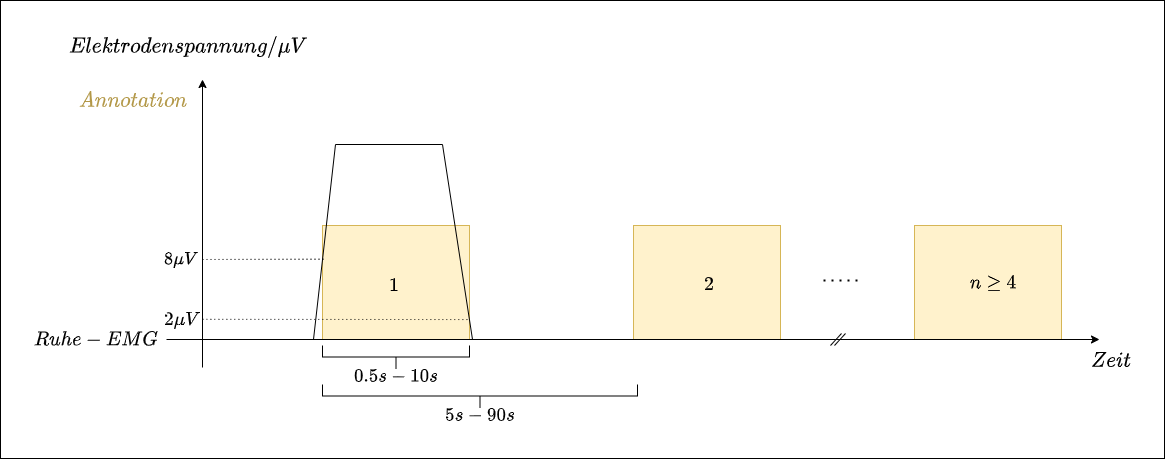
\includegraphics[width=0.80\textwidth]{./Bilder/AASMLM.drawio (2).png}
	\end{center}
	\caption{Graphische Veranschaulichung der AASM-Kriterien.}%
	\label{fig:AASMKrit}%
\end{figure}
Die Muskelaktivität spielt auch bei folgenden Symptomen eine Rolle, muss aber von diesen abgegrenzt werden: hypnagogem Fußzittern (Hypnagogic Foot Tremor), alternierender Beinmuskelaktivität (Alternating Leg Muscle Activation, ALMA), exzessivem fraktionierten Myoklonus im NonREM-Schlaf, phasischen REM-twitches und Wadenkrämpfen \cite{PDS}. Die Kriterien zur Unterscheidung von anderen Bewegungsstörungen sind in \cite{AASM} beschrieben.

Die Beinbewegungen können mit Arousals einher gehen, welche zu einer partiellen, temporären oder vollständigen Weckreaktion führen. Diese äußern sich durch eine abrupte Frequenzänderung im Elektroenzephalogramm und sollen, laut der AASM, den Beinbewegungen zugeordnet werden. Da die Beinbewegungen überwiegend in den Schlafstadien N1 und N2 auftreten und oft mit Weckreaktionen einhergehen, sind REM- und Tiefschlaf häufig vermindert. Darunter leidet die Schlafeffizienz und die gesunde Periodizität der Schlafphasen wird gestört. Bei länger anhaltenden Beschwerden entwickeln viele Patienten zusätzlich psychische Fehlhaltungen und Verhaltensweisen, die die Schlafqualität weiter verschlechtern. Der Schlaf ist dadurch weniger erholsam. Es kommt zu Symptomen einer Hypersomnie, wie zum Beispiel eine ausgeprägte Tagesschläfrigkeit und Monotonieintoleranz sowie sekundäre depressive Symptome, imperative Einschlafattacken, Gedächtnis- und Aufmerksamkeitsstörungen. Diese können den Alltag stark beeinträchtigen und beispielsweise beim Autofahren sogar tödlich sein. Darüber hinaus werden die PLM mit Herzkrankheiten, hohem Blutdruck und Herzversagen assoziiert \cite{Huang}. \cite{PDS}

In der Praxis wird der PLMS-Index, also die Anzahl der pro Stunde auftretenden periodischen Beinbewegungen im Schlaf, genutzt, um das Ausmaß einer möglichen Erkrankung festzustellen. Dabei gelten bis zu fünf pro Stunde als unauffällig, zwischen fünf pro Stunde und ≤20 pro Stunde als leichte Störung, zwischen 20 pro Stunde und 60 pro Stunde als moderate Störung und bei einem PLMS-Index über 60 pro Stunde als schwere Erkrankung. \cite{PDS}


\section{Ursachen}
Periodische Beinbewegungen sind Symptome vieler unterschiedlicher Krankheiten. Diese treten beim \gls{RLS} in 80 Prozent der Fälle, bei der REM-Verhaltensstörung in 70 Prozent und bei Narkolepsie in 45 Prozent bis 60 Prozent der Fälle auf. Bei der Krankheit Insomnie sind in 1 Prozent bis 15 Prozent der Fälle periodische Beinbewegungen symptomatisch und bei einer obstruktiven Schlafapnoe sind auch oft PLM vorhanden. Außerdem werden diese häufig in Assoziation mit psychiatrischen Störungen und bei neurologischen Erkrankungen wie Multisystematrophie oder Rückenmarksverletzungen gefunden. Auch Nebenwirkungen durch eingenommene Medikamente sind möglich. Dies ist allerdings nur eine Auswahl aller möglichen Ursachen. Falls das Symptom nicht durch eine der obigen Krankheiten erklärt werden kann, wird die Diagnose "Periodic-Limb-Movement-Disorder" gestellt, auch wenn die Krankheiten simultan auftreten können \cite{1x1}. \cite{PDS}

Da die Krankheitsbilder sehr unterschiedlich sind, sind auch die Ursachen für periodische Beinbewegungen vielfältig. Bei dem RLS und PLMD ist die Erkrankung ähnlich, aber noch weitgehend unverstanden. Diese entsteht wahrscheinlich im Zentralnervensystem durch eine Störung des dopaminergen oder opioidergen Systems \cite{1x1}, welche durch eine Störung des Eisenstoffwechsels auftreten könnte. Diese These wird gestützt durch das vermehrte Auftreten von PLM im höheren Alter bei einem gleichzeitigen Verlust an Dopamin und Dopaminrezeptoren. Die mit RLS korrelierenden Gene könnten auf eine frühe Entwicklungsstörung des zentralen Nervensystems hindeuten. \cite{PDS}

\section{Therapie}

Periodische Beinbewegungen sollen nur dann behandelt werden, wenn sie eine Insomnie oder Hypersomnie auslösen, welche nicht durch andere Erkrankungen erklärt werden kann. Grundsätzlich gilt, dass nach Möglichkeit zuerst die Grunderkrankung behandelt werden sollte, falls diese in Verbindung mit PLM auftritt. \cite{PDS}

Das RLS und PLMD werden pharmakologisch behandelt, indem die oben beschriebenen Mängel ausgeglichen werden. Hier soll zuerst dopaminerg, danach antiepileptisch und als letzte Maßnahme opioiderg behandelt werden. Hier eignen sich die Wirkstoffe L-Dopa, Rotigotin und Oxycodon je nach Schweregrad. Zusätzlich ist eine Eisensubstitution empfehlenswert. Insomnien sollten generell mit nichtmedikamentösen Verfahren kombiniert werden, indem über Grundlagenwissen der Schlafhygiene (z.B. Zubettgeh-Ritual, Matratze, Raumtemperatur, Geräuschisolierung und Abdunkelungsmöglichkeiten) aufgeklärt wird. Die Verwendung von schlaffördernden Mitteln wirkt lediglich symptomatisch und sollte nur über einen begrenzten Zeitraum erfolgen. \cite{1x1,PDS}

Die meisten Krankheitsbilder werden in erster Linie durch Fragebögen festgestellt. Die periodischen Beinbewegungen werden jedoch in der Regel nicht durch den Patienten in der Nacht wahrgenommen. Eine mögliche schlafstörende Wirkung kann durch ein Elektroenzephalogramm bestätigt werden. Dies ist nötig, da sonst keine Therapie verschrieben werden darf. Bei diagnostisch unklaren Fällen, sowie bei Kindern und Jugendlichen kann es auch gerechtfertigt sein, den Schlaf im Schlaflabor zu überwachen. \cite{1x1}


\section{Biophysikalischer Signalursprung}

In der folgenden Arbeit werden Daten aus Elektromyogrammen ausgewertet. Deswegen ist es an dieser Stelle wichtig, zu verstehen, welchen biophysikalischen Ursprung die ausgewerteten Signale haben. 
Da Beinbewegungen im PSG nicht direkt gemessen werden können, werden im Schlaflabor ersatzweise die Muskelkontraktionen des Beines gemessen, welche die Bewegungen verursachen. Um in diesem Kontext eine Muskelkontraktion zu verursachen, muss zunächst ein Signal in Form eines Aktionspotentials einer Nervenzelle zu dem Muskel weitergeleitet werden. Diese Nervenzelle bewirkt eine Depolarisation in der anliegenden Muskelzelle, in der Calciumionen freigesetzt werden \cite{biomechanist}. Die Calciumionen ermöglichen dann die Kontraktion des Muskels \cite{motorischeEndplatte}. Dieser Vorgang verändert das Potentialfeld, welches an der Hautoberfläche mit einer Elektrode gemessen werden kann. Die Änderung ergibt sich aus der Überlagerung der Depolarisation von Nerven- und Muskelzellen, welche anschließend durch aktives Zurückpumpen von Calciumionen repolarisiert werden \cite{motorischeEndplatte}. Da Muskeln aus vielen Fasern bestehen, welche jeweils nur kurz und mehrfach an einer Kontraktion des gesamten Muskels beteiligt sind, ist die Potentialänderung ein stochastisches Signal in einem Frequenzbereich von zwischen zehn Hertz und 500 Hertz \cite{Mehrkanal-BioimpedanzInstrumentierung}. Die ein bis drei Quadratmillimeter große Depolarisationszone wird mit einer Geschwindigkeit von zwei bis sechs Meter pro Sekunde entlang der Muskelfaser weitergeleitet \cite{biomechanist}.
Laut AASM sollen die Kontraktion beider Beine anhand jeweils zweier Elektroden gemessen werden, welche entlang des Tibialis Anterior Muskels (Tibialis anterior muscle) platziert sind \cite{AASM}. 

\section{Störgrößen}
Der Vorteil in der Nutzung zweier Elektroden ergibt sich aus der verbesserten Unterdrückung von Störgrößen. Das Signal ist dadurch im Idealfall unabhängig von Einflussgrößen, welche auf beide Elektroden wirken und daher nicht von dem gewünschten Signal verursacht wurden. Diese Störgrößen beinhalten das statische Potentialfeld, Haut-Elektrode Übergänge, kapazitive und induktive Einkopplung von anderen elektrischen Geräten und der Netzspannung. 
Im Idealfall heben sich die Halbzellspannungen auf, welche durch den Elektrode-Haut-Übergang entstehen. Die oben genannten Gleichtaktstörgrößen beeinflussen das Signal jedoch wenig, falls die Bioimpedanzen klein sind im Vergleich zu der Innenimpedanz des Messinstruments. Die AASM empfiehlt Impedanzen von 5000 Ohm \cite{AASM}. \cite{Mehrkanal-BioimpedanzInstrumentierung}

Problematisch sind auch zeitliche Änderung der Haut-Elektrode Übergänge, welche durch die Bewegung oder Schweiß entstehen können \cite{Mehrkanal-BioimpedanzInstrumentierung,PRT}.
Zwischen dem Muskel und der Elektrode befindet sich weiteres Gewebe, welches das Signal nichtlinear verzerren kann und wie ein Tiefpass Filter wirkt, dessen Grenzfrequenz mit der Gewebedicke abnimmt. Eine weitere Störgröße ist die Überlagerung von Potentialfeldern, welche durch das Herz oder die Atmung verursacht wurden \cite{Moore,1x1}. \cite{physiology}

Das Schlafverhalten des Patienten ist möglicherweise aufgrund der Verkabelung und Überwachung im Schlaflabor gestört \cite{1x1}. Zudem kann es selbst bei einer schweren Erkrankung Nächte geben, in denen wenig periodische Beinbewegungen auftreten \cite{PDS}.
 \newpage


\chapter{Stand der Technik}\label{chap:Stand_der_Technik}
\section{Datenverarbeitungskette}

Die Datenerhebung findet über eine Polysomnographie im Schlaflabor statt. Richtlinien dazu finden sich in der \cite{AASM}. In einer Standarduntersuchung werden ein Elektroenzephalogramm (EEG), ein Elektrookulogramm und Elektromyogramme (EMG) erstellt \cite{1x1}. Das EMG besteht aus den Elektroden, einer Verstärkerschaltung, einem Analog-Digital-Umsetzer und Filtern \cite{biomechanist} \cite{PRT}. Der Analog-Digital-Umsetzer soll mit mindestens 200 Hertz (möglichst mit 500 Hertz) und einer 12 Bit Quantisierung arbeiten \cite{AASM}. Üblich sind heutzutage 16 bis 22 Bit \cite{SleepDisordersMedicine}.

Außerdem können bei Bedarf 50 Hz beziehungsweise 60 Hz (in Amerika) Notchfilter eingesetzt werden. Die AASM rät davon allerdings ab, da die Aufzeichnung der Muskelaktivität beeinträchtigt werden könnte \cite{PRT}.
Der Start der eigentlichen Messung beginnt mit dem Löschen des Lichtes (Licht aus) und endet mit dem Anschalten des Lichtes (Licht an) \cite{1x1}. Die Aufzeichnung wird auf den Monitoren mit einer Geschwindigkeit von zehn Millimeter pro Sekunde dargestellt, sodass auf einen Bildschirm 30 Sekunden passen \cite{PRT}. Die Einteilung ist historisch aus den Aufzeichnungen auf Endlospapier entstanden, welches nach 30 Sekunden umklappte. Die gesammelten Daten werden anschließend verwendet, um unter anderem motorische, respiratorische und EEG-bezogene Ereignisse zu finden und zu klassifizieren. \cite{PDS}

Die Software der Aufzeichnungsgeräte verfügt meistens direkt über eine Annotationsunterstützung, welche Vorschläge für die Start- und Endzeitpunkte der Beinbewegungen (LM) macht. Diese werden vom Assistenzpersonal überarbeitet. Vorschläge, die mit atembezogenen Events (zum Beispiel einer Schlafapnoe) zusammenhängen, sollen laut AASM gelöscht werden. Abschließend werden Regeln zur Bestimmung von periodischen Beinbewegungen angewandt (siehe Kapitel: „medizinische Grundlagen“), um die PLMS-Kennwerte zu bestimmen (Anzahl von PLMS, Anzahl von PLMS mit Arousals, PLMS-Index, PLMS-Arousal-Index) \cite{Carvelli}. Die Annotationen werden später von einem Somnologen oder von einem Arzt für Schlafmedizin überprüft \cite{PDS}. \cite{PRT}

In dem Prozessbild \ref{fig:Prozessbild} ist die Datenverarbeitungskette dargestellt. Als Eingangssignal auf der linken Seite ist das EMG Signal aus dem Schlaflabor zu sehen, welches durch das medizinische Personal -meist mithilfe der Annotationsunterstützung- auf Beinbewegungen untersucht wird. Durch die Verarbeitung entsteht ein binäres Annotationssignal, welches jedem Zeitpunkt aus dem ursprünglichen EMG-Signal zuweist, ob an diesem Zeitpunkt eine Beinbewegung vorliegt oder nicht. Anhand dieses Annotationssignals wendet ein Algorithmus die Kriterien der AASM an und berechnet Kennwerte, die repräsentativ für das Annotationssignal stehen.


\begin{figure}[!ht]%
	\begin{center}
	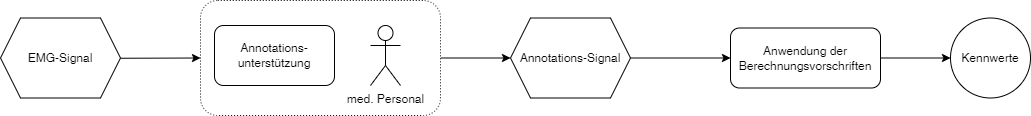
\includegraphics[width=0.80\textwidth]{./Bilder/Prozessbildrot.drawio.png}
	\end{center}
	\caption{Veranschaulichung der Datenverarbeitungskette. Das EMG-Signal wird von medizinischem Personal mithilfe von Annotationsunterstützung verarbeitet. Rechts im Bild sind die Kennwerte dargestellt, die von einem Algorithmus berechnet werden und das Ergebnis der Kette beschreiben.}%
	\label{fig:Prozessbild}%
\end{figure}

\section{Detektoren}
Die Detektoren können nach der Art der Vorverarbeitung der Eingangsdaten, der Merkmalsextraktion und der Klassifizierung unterschieden werden. Es gibt sehr unterschiedliche Möglichkeiten die Merkmalsextraktion umzusetzen. Sie kann beispielsweise im Frequenzbereich (spektrale Kantenfrequenz\footnote{Frequenz unter der ein bestimmter Prozentsatz der Gesamtleistung liegt.}, fraktaler Exponent\footnote{Maß für Signalkomplexität: Steigung der Geraden in der doppeltlogarithmischen Darstellung spektrale Leistungsdichte gegen Frequenz \cite{dirichlet}.}) \cite{dirichlet}, im Zeit-Frequenzbereich (Waveletkoeffizienten) \cite{shroko} oder im Zeitbereich (Spikewiederholrate, durchschnittliche Amplitude, Länge des Zeitfensters in dem Spikes auftreten) \cite{wetter} stattfinden. Die Auswertung kann zum Beispiel über statistische Klassifikatoren \cite{probabilistic,dirichlet} oder Neuronale Netze \cite{Carvelli,shroko} erfolgen.

Am meisten verbreitet sind die Detektoren, die im Zeitbereich eine Schwellwertklassifikation mit einem absoluten \cite{wetter,ferri,Huang,stefani,tauchmann} oder dynamischen \cite{alvarez,Moore} Schwellwert vornehmen. Hierbei wird meist die Amplitude des vorverarbeiteten Signals als Merkmal genutzt. Der Detektor von Carvelli et al. nutzt ein \gls{DNN} für die Klassifikation.

Für ein besseres Verständnis der Funktionsweise wird im Folgenden der Algorithmus von Moore et al. zusammengefasst. Dieser wurde gewählt, da der Ansatz weit verbreitet ist und Ideen von Tauchmann, Ferri et al. und Wetter et al. aufgegriffen und weiterentwickelt wurden. 


\begin{enumerate}
	\item Einlesen des Datensatzes
	
	Die beiden EMG-Signale der Beine werden zu einem Signal zusammengeführt und die Elektrokardiogrammstörung mithilfe eines adaptiven Filters vermindert.
    Das gesäuberte Signal wird gleichgerichtet zu x(n).
    Für die Annotation wird das RMS y(n) von x(n) mit einem beidseitigem 0.15-sekündigen Fenster gebildet. 

	\item Berechnung des Grundrauschens
	
	Aus dem x(n) wird mithilfe eines 20-sekündigen gleitenden Mittelwertes das vorläufige Grundrauschen $\eta$ (n) ermittelt. Das Grundrauschsignal ist nur vorläufig, da alle Beinbewegungen mit in den Mittelwert eingerechnet werden und somit fälschlicherweise das Grundrauschen erhöhen. 
    Aus dem Grundrauschen wird auch der vorläufige erste und zweite Schwellwert berechnet ($\alpha$ und $\beta$)
    \[ \alpha(n) = \left\{\begin{matrix}\eta(n)\log(\eta(n)+1)+U \\\infty \end{matrix}
    \right.\begin{matrix}, \eta\leq 50\\, \eta> 50
    \end{matrix}\]
    \[ \beta(n) = \frac{L}{U} \alpha(n) \]


    \item Berechnung der Annotation
        
    Diese Schwellwerte weichen bewusst von den definierten Werten der AASM Kriterien ab, orientieren sich jedoch an diesen durch die Startwerte L und U. Der Startzeitpunkt für einen Beinbewegungskandidaten ist der Zeitpunkt, bei dem y(n) das erste Mal den oberen Schwellwert überschreitet. Die Beinbewegung endet, wenn das RMS-Signal für 0.05 Sekunden unter dem unteren Schwellwert bleibt. Kandidaten, die weniger als 0.1 Sekunden voneinander trennt, werden zusammengefasst. 
    Um den Verlauf des Grundrauschens besser zu approximieren, wird an den Stellen, an denen Beinbewegungenskandidaten erkannt wurden, der Wert des absoluten EMG-Signals auf die Hälfte des zweiten Schwellwertes $\beta$(n) gesetzt. Dieses Signal ist das finale Grundrauschen.
    
\end{enumerate}



\section{Klassische Metriken}



Die Metriken können segmentweise oder eventweise berechnet werden. Ein Segment wird meist als positiv gezählt, wenn das binäre quasizeitkontinuierliche Signal bei mehr als 50\% des Segmentzeitraumes positiv ist. Wenn die Segmente die Länge eines Abtastzeitraumes haben, geht die segmentweise Klassifikation in eine sampleweise Klassifikation über.
Bei der eventweisen Klassifikation erfolgt die Zuordnung analog. Hier wird jedoch meistens (mit Ausnahme von \cite{stefani}) ein TP gezählt, sobald sich die beiden Annotationszeiträume mit mindestens einem Abtastwert überlappen. Dabei kann es passieren, dass mehrere Events in einem Signal auftreten, während in der anderen Annotation nur ein Event gefunden wurde. Hier findet eine multiple Zuordnung statt, bei der für alle dieser Events ein TP gezählt wird. Die Notation ist analog zu Wetter et al. mit Xto1-Matching bei mehreren manuellen Annotationen und 1toX-Matching bei mehreren automatischen Annotationen.

Die Abbildung \ref{fig:Zuordnung} gibt einen Überblick über die segmentweise und eventweise Klassifikation zusammen. Zu beachten ist, dass die Events in der Auswertung nicht mit ihrer Zeit gewichtet werden, sondern nur gezählt werden. 

\begin{figure}[!ht]%
	\begin{center}
	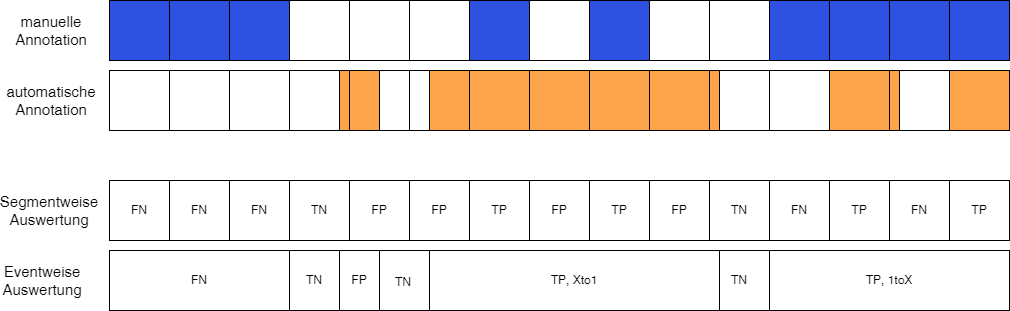
\includegraphics[width=0.80\textwidth]{./Bilder/Zuordnung.png}
	\end{center}
	\caption{Klassifizierung von \gls{TP}, \gls{TN}, \gls{FP} und \gls{FN} nach segement- und eventweiser Berechnung bei segemtierter manueller und quasizeitkontinuierlicher automatischer Annoatation.}%
	\label{fig:Zuordnung}%
\end{figure}

Die wichtigsten klassischen Metriken aus der Literatur werden im Folgenden vorgestellt.\\

\noindent\textbf{\gls{rr} (PLM/h)}\\ 
\begin{equation}\frac{ \sum_{i=1}^{n} (x_i - \Bar{x})(y_i - \Bar{y})}{\sqrt{\sum_{i=1}^{n} (x_i - \Bar{x})^{2}} \sqrt{\sum_{i=1}^{n} (y_i - \Bar{y})^{2}}}\end{equation}\\
\textbf{Cohens $\kappa$}\\
\begin{equation}
P_e = \frac{(TP+FN)(TP+FP)+(TN+FP)(TN+FN)}{(TP+TN+FP+FN)^{2}}\\\end{equation}
\begin{equation}P_0 = \frac{TP+TN}{2}\\\end{equation}
\begin{equation}\kappa = \frac{P_0 - P_e}{1-P_e}\\\end{equation}
\textbf{F1-Ma"s}\\
\begin{equation}\frac{2TP}{2TP+FP+FN}\\\end{equation}
\textbf{AUROC}\\
Integral unter der Grenzwertoptimierungskurve beim Verändern des Entscheidungsschwellwertes\\
\textbf{AUPRC}\\
Integral unter der Genauigkeits-Sensititvitäts-Kurve beim Verändern des Entscheidungsschwellwertes\\
\textbf{\gls{Prec}}\\
\begin{equation}\frac{TP}{TP+FP}\\\end{equation}
\textbf{\gls{NPV}}\\
\begin{equation}\frac{TN}{TN+FN}\\\end{equation}
\textbf{\gls{Acc}}\\
\begin{equation}\frac{TP+TN}{TP+TN+FP+FN}\\\end{equation}
\newpage
\noindent
\textbf{\gls{Sens}}\\
\begin{equation}\frac{TP}{TP+FN}\\\end{equation}
\textbf{\gls{Spez}}\\
\begin{equation}\frac{TN}{TN+FP}\\\end{equation}
\textbf{\gls{FPrate}}\\
\begin{equation}\frac{FP}{FP+TP}\\\end{equation}


Die Tabellen \ref{tab:Stand der Technik1} und \ref{tab:Stand der Technik2} beschreiben den Stand der Technik und geben einen Überblick welche Detektoren aus der Literatur bereits welche Ergebnisse erzielen konnten.

\begin{table}[!ht]
    \caption{Stand der Technik, Teil 1; Der Zusatz 'r' bezeichnet einen rekonstruierten Wert}   
	\centering
		\begin{tabular}{llllllllll}
			\hline & \cite{Huang} & \cite{Moore} & \cite{Moore} & \cite{alvarez} & \cite{ferri}\\
			\hline {$\!\begin{aligned}
				&\\
			    Datensatz\\
			    Art\ des\ Klassifikators\\
			    Berechnungsart\\
			    \gls{Sens}\\
			    \gls{Prec}\\
			    \gls{Spez}\\
			    \gls{NPV}\\
			    \gls{Acc}\\
			    Cohens\ \kappa\\
			    F1-Ma"s\\
			    Korrealtion\ PLM/h\\
			    relative\ \#\ PLM\\
				&\\
				\end{aligned}$} & {$\!\begin{aligned}
				&\\
				15\ \gls{RLS}\ (24)\\
				statisch\\
				Event\\
				0.95\\
				-\\
				0.92\\
				-\\
				-\\
				-\\
				0.93r\\
				0.97\\
				1.05\\
				&\\
				\end{aligned}$} & {$\!\begin{aligned}
				&\\
				\acrshort{WSC}\ (1073)\\
				dynamisch\\
			    Event\ \cite{git}\\
				0.6\\
				0.88\\
				1\\
				0.99\\
				0.98\\
				0.71\\
				-\\
				0.94\\
				0.63\\
				&\\
				\end{aligned}$} & {$\!\begin{aligned}
				&\\
				\acrshort{SSC}\ (760)\\
				dynamisch\\
				Event\ \cite{git}\\
				0.75\\
				0.82\\
				1\\
				0.99\\
				0.99\\
				0.87\\
				-\\
				0.94\\
				0.92\\
				&\\
				\end{aligned}$}  & {$\!\begin{aligned}
				&\\
			    \acrshort{HMC}\ (70)\\
				dynamisch\\
				Segment\ (1s)\\
				0.82\\
				0.71\\
				1\\
				-\\
				1\\
				0.73\\
				0.73\\
				-\\
				0.99\\
				&\\
				\end{aligned}$}  & {$\!\begin{aligned}
				&\\
				\acrshort{WSC}\ (60)\\
				statisch\\
				Event\\
				0.85\\
				0.62\\
				0.99\\
				1\\
				0.99\\
				0.72\\
				-\\
				-\\
				1.33\\
				&\\
				\end{aligned}$}
				\\
				\hline
		\end{tabular}

\label{tab:Stand der Technik1}
\end{table}

\begin{table}[!ht]
    \caption{Stand der Technik, Teil 2}   
	\centering
		\begin{tabular}{llllllllll}
			\hline & \cite{wetter} & \cite{Carvelli}& \cite{Carvelli}& \cite{Carvelli}\\
			\hline {$\!\begin{aligned}
			    &\\
			    Datensatz\\
			    Art\ des\ Klassifikators\\
			    Berechnungsart\\
			    \gls{Sens}\\
			    \gls{Prec}\\
			    \gls{Spez}\\
			    \gls{NPV}\\
			    \gls{Acc}\\
			    Cohens\ \kappa\\
			    F1-Ma"s\\
			    Korrealtion\ PLM/h\\
			    relative\ \#\ PLM\\
				&\\
				\end{aligned}$} & {$\!\begin{aligned}
				&\\
				\acrshort{WSC}\ (60)\\
				statisch\\
				Event\\
				0.96\\
				0.47\\
				0.98\\
				1\\
				0.98\\
				0.62\\
				-\\
				-\\
				2.05\\
				&\\
				\end{aligned}$} & {$\!\begin{aligned}
				&\\
                \acrshort{WSC}\ (275)\\
				\acrshort{DNN}\\
				Event\\
				0.9\\
				0.81\\
				-\\
				-\\
				-\\
				-\\
				0.83\\
				-\\
				-\\
				&\\
				\end{aligned}$}& {$\!\begin{aligned}
				&\\
                \acrshort{SSC}\ (177)\\
				\acrshort{DNN}\\
				Event\\
				-\\
				-\\
				-\\
				-\\
				-\\
				-\\
				0.71\\
				-\\
				-\\
				&\\
				\end{aligned}$}& {$\!\begin{aligned}
				&\\
                MrOS\ Sleep\ Study\ (348)\\
				\acrshort{DNN}\\
				Event\\
				-\\
				-\\
				-\\
				-\\
				-\\
				-\\
				0.77\\
				-\\
				-\\
				&\\
				\end{aligned}$}
				\\
				\hline
		\end{tabular}

\label{tab:Stand der Technik2}
\end{table}


Bei der eventweisen Berechnungsart wurde ein TP bei jeglicher Überlappung gewertet. Die Werte für den Detektor von Wetter et al. sind aus \cite{Moore} übernommen.
Der Zahlenzusatz 'r' steht dafür, dass dieser Wert nicht veröffentlicht wurde, aber aus den anderen Metriken rekonstruiert werden konnte.
Die Zahl in Klammern am Ende der Datensatzbeschreibung bezeichnet die Gesamtanzahl der Patienten im verwendeten Datensatz. \newpage
\input{Subfiles/Präzisierung_der_Aufgabenstellung} \newpage
\chapter{Wahl der Metrik}\label{chap:Wahl_der_Metrik}
\section{Klassische Metriken}
Bei der Berechnung jeder Metrik gehen Informationen verloren, da zwei zeitliche Signale, welche jeweils komplizierte Zusammenhänge zwischen den einzelnen Events haben, auf eine reelle Zahl abgebildet werden. 
Also sollte man genau betrachten, welche Informationen bei dem Berechnen der klassischen Metriken verloren gehen.

Das Ziel der poysomnographischen Untersuchung und Auswertung ist es, die klinischen Kennzahlen der AASM \cite{AASM} aus dem Annotationssignal zu bestimmen, um herauszufinden, wie stark ein Krankheitsverlauf den Schlaf stört. Daher wäre es sinnvoll den Detektor an dem Vergleich dieser Kennzahlen zu bemessen.
Der Vergleich der Kennzahlen liefert allerdings kein vollständiges Bild über die korrekte Arbeitsweise des Detektors. Die Kennzahlen werden bei dem Detektor aus \gls{TP}- und \acrfull{FP} Werten berechnet. Letztere sind allerdings nicht durch eine korrekte Arbeitsweise entstanden, sondern durch einen Fehler des Detektors.


Für die Bewertung des Annotationssignales kann die Berechnung von \gls{TP}, \gls{FP}, \gls{TN} und \gls{FN} Werten segementweise oder eventweise geschehen. 

Selbst bei einer schweren Erkrankung mit einem PLM-Index von 60 pro Stunde \cite{PDS} und maximaler Beinbewegungslänge von zehn Sekunden liegt das Verhältnis von Beinbewegungen zu Ruhephasen bei circa eins zu fünf. Bei einer segmentweisen Berechnung hätte also eine starke Ungleichverteilung in beiden Klassen. Da die Anzahl der TN sehr hoch sein wird, bieten Sensitivität, Spezifität, und Korrektklassifikationsrate keinen informativen Gehalt \cite{Huang}. 
Die Länge der jeweiligen LM ist für medizinische Entscheidungen nicht relevant. Da nur die Anzahl (und Abstände) der Events zählen, ist es sinnvoller die Metriken eventbasiert zu berechnen.
Bei dieser zählweise sind die Klassen wesentlich gleicher verteilt, da gilt: TP + FP + 1 = TN + FN (falls die Ränder negativ sind). 

Die Metriken, die sich anhand des Annotationssignales berechnen lassen, sind eher ungeeignet, um einem Detektor eine Güte zuzuweisen. Bei den Metriken Genauigkeit, Spezifizität und negativem Vorhersagewert fehlt jeweils eine der vier Klassen, weswegen die Werte einzeln betrachtet den Detektor nicht gut repräsentieren. Beispielsweise wäre die Sensitivität perfekt auf dem Wert 1 wenn der Detektor jeden Abtastwert als Beinbewegung klassifiziert. 
Es kann außerdem passieren, dass die klassischen Metriken unendlich große Werte annehmen beziehungsweise neu definiert werden müssten.
Dies kommt zum Beispiel bei der Genauigkeit zustande, wenn weder TP noch FP gefunden wurden. 

Die klassischen Metriken lassen auch nicht immer eine eindeutige Aussage zu. Beispielsweise ist die Sensitivität bei dem Detektor von Huang et al. größer als die bei dem Detektor von Moore et al. Bei der Spezifizität verhält es sich umgekehrt. 
Zudem lassen sich die Metriken sehr schlecht untereinander vergleichen, wenn sie auf unterschiedlichen Datensätzen berechnet werden. \cite{jamareyna} 

Andere Metriken wie Cohens $\kappa$ beinhalten zwar alle der vier Klassen und gelten als aussagekräftig, jedoch geht durch die komplexe, abstrakte Berechnungsweise die Nachvollziehbarkeit und Erklärbarkeit verloren.
Das Integral unter der ROC-Kurve sowie das Integral unter der Genauigkeits-Sensititvitäts Kurve bieten für viele Arten von Detektoren eine gute Aussagekraft, sind jedoch für den Vergleich von Detektoren, welche auf Schwellwerten basieren, nicht anzuwenden.
Ein Effekt der eventweisen Berechnung ist außerdem, dass im Normalfall (isolierte Events) durch ein FP immer ein weiteres TN entsteht (im Vergleich zu dem Fall, dass es das FP nicht gegeben hätte). Genauso geht durch ein FN ein TN verloren. 
Dies führt dazu, dass die klassischen Metriken nicht die Aussage treffen, nach der es beim Betrachten der Formeln aussieht. Hier geht die Information verloren, wodurch (hier) das TN entstanden ist.

Die klassischen Metriken als Gesamtes betrachtet haben eine gewisse Aussagekraft, wenn alle der klassischen Metriken ausreichend hoch sind, da beispielsweise bei einem sehr hohen F1-Maß die errechneten Kennwerte fast ausschließlich aus den richtig erkannten Beinbewegungen stammen müssen. Komplizierter wird es allerdings, wenn die klassischen Metriken zweier Detektoren ähnlich sind oder nicht ausreichend gut. In diesen Fällen ist die Informationsreduktion in den klassischen Metriken zu groß, um fundierte Aussagen über die jeweiligen Detektoren treffen zu können.
Der Detailgrad der Information beschränkt sich jedoch auf vage Aussagen wie „Sensitivität ist höher als Genauigkeit, was signalisiert, dass das Modell sehr inklusiv ist“ \cite{Carvelli}.
Außerdem muss für die Definition einer Güte ein skalarer Wert definiert werden. 
Ein weiteres Problem ist, dass zeitliche Zusammenhänge zwischen den Events verloren gehen. Die Berechnung der medizinisch wichtigen Kennwerte ist jedoch teilweise durch die Zeiten zwischen den LM-Startzeiten relevant. Deswegen lassen sich nicht alle Informationen aus der Anzahl der TP, TN, FP und FN-Werte ableiten.

\section{Kostenfunktional}

Es wird also eine neue Metrik benötigt, welche die Kriterien im Ziel der Arbeit besser erreicht.
Das Konstenfunktional ist hier definiert als eine Funktion, welche zwei binäre Annotationssignale auf ein Skalar abbildet. Dieser Skalar beschreibt die Fehler (Kosten), die von einem Detektor gemacht wurden beim berechnen des automatischen Annotationssignals im Vergleich zu dem manuellen Annotationssignal.
Die Güte (G) um den Detektor zu beschreiben kann reziprok zu den Kosten (K) definiert werden: \begin{equation}
    G = \frac{1}{1+K}\label{Güte}
\end{equation}. Diese Definition hat den Vorteil, dass die Güte in einem Wertebereich zwischen Null und Eins liegt. 

Für die Beschreibung des Kostenfunktionals in dieser Arbeit wird sich auf den PLMS/h als medizinisch relevanten Wert beschränkt. Die Berechnungsweise lässt sich leicht erweitern, um andere Indices zu beschreiben.
Das Kostenfunktional soll die aufgezeigten Probleme mit den herkömmlichen Metriken lösen, indem die Fehler gezählt werden, die gemacht wurden beim Bestimmen des PLMS-Indexes. 


Für die Bestimmung der Fehler ist es zunächst notwendig, die Beinbewegungen zu finden, welche von dem Detektor richtig erkannt wurden. Für den Menschen ist es intuitiv zu wissen welche Beinbewegungen von dem Detektor „gemeint“ sind. Diese Intuition ist vermutlich von der Umgebung der Beinbewegungen abhängig. So würden LM einander großzügiger zugeordnet werden, wenn sich in der Umgebung keine weiteren LM befinden. Ist jedoch die Eventdichte hoch, würden strengere Regeln gelten. Für die Anwendung auf die Detektoralgorithmen ist dieses Vorgehen eher unbrauchbar. In der Literatur wird meistens ein TP gezählt, wenn ein Abtastwert von beiden Annotationen als positiv eingestuft wird. Dieser Ansatz wird hier übernommen.
Dabei kann es passieren, dass die manuelle Annotation für einen Zeitraum nur ein LM vorsieht, der Detektor aber mehrere findet (1toX-Matching). Umgekehrt kann werden auch alle manuellen Annotationen, die mit einer automatischen Annotation überlappen dieser zugeordnet (Xto1-Matching).
\\
 
\noindent Für eine zu hohe PLM Anzahl kann es folgende Gründe geben:



\begin{enumerate}
	\item Vorhandensein eines FP innerhalb einer PLMS-Serie in [5-90] Sekunden Abstand zu einem zugehörigen LM
	\item Dazuzählen eines TP, da es fälschlicherweise in das [5-90] Sekunden Intervall zählt
	\item Vorhandensein von 1toX-Matching
	\item Gründung einer PLM-Serie durch oben genannte Gründe
\end{enumerate}



\noindent Für eine zu kleine PLM-Anzahl kann es folgende Gründe geben:

\begin{enumerate}
	\item Vorhandensein eines FN in [5-90] Sekunden Abstand zu einem PLM
	\item Nichtinkludieren eines TP, da es sich nicht in dem [5-90] Sekunden Intervall befindet
	\item Vorhandensein von Xto1-Matching
	\item PLM-Serie kommt nicht zu Stande aus oben genannten Gründen
\end{enumerate}


Die Mengen FP und TP sind disjunkt und es kann deswegen nicht zu doppelten Zählungen kommen. Da die 1toX-Matches ein Teil der TP sind, gibt es beispielsweise einen Grenzfall, bei dem der erste oder letzte LM eines 1toX-Matches sich innerhalb des [5-90] Sekunden Intervalls befindet, das LM der manuellen Annotation jedoch noch nicht. Die Umsetzung des Kostenfunktionals speichert die Beinbewegungen, die bereits zu einer Veränderung des Indexes beigetragen haben, sodass diese nicht doppelt gezählt werden.
 
Die Punkte eins bis drei tragen direkt zu einer Veränderung des PLM Indexes bei. Die Fehler unter Punkt vier tragen nichtlinear zum Ergebnis bei, da eine PLM-Serie wird erst als solche gezählt wird, wenn mindestens vier LM zu dieser Serie gezählt werden. Falls durch einen Fehler beispielsweise sich nur drei anstatt vier LM in der Serie befinden, wird das Ergebnis durch nur einen Fehler um vier verringert anstatt nur um eins. Das Kostenfunktional soll in diesem Fall auch die Veränderung der PLM Anzahl wiederspiegeln. 


Die Arbeitsweise des Kostenfunktionals lässt sich anhand eines hypothetischen Annotationssignal gut veranschaulichen. In den folgenden Beispielen wurde ein Ausschnitt eines manuellen Annotationssignals aus dem Datensatz verwendet, welches eine PLM-Serie mit insgesamt vier PLM aufweist.  
Das erste automatische Beispielsignal ist in Bild \ref{fig:all1} dargestellt und besteht nur aus einem LM, welches über die ganze Nacht andauert. Für einen Vergleich wurde in diesem Abschnitt zusätzlich ein manuell annotiertes Beispielsignal aus dem Datensatz \ref{chap:Datensatz} verwendet.

Die klassischen Metriken kommen hier bei der eventweisen Berechnung auf einen Wert von eins und treffen damit die Aussage, dass der Detektor perfekt funktioniert. Das Kostenfunktional hingegen berechnet absolute Kosten von vier, da die manuelle Annotation aus vier PLM besteht und keine Serie richtig erkannt wurde. Die Fehler wurden alle richtigerweise Xto1-Matches klassifiziert. 


\begin{figure}[!ht]%
	\begin{center}
	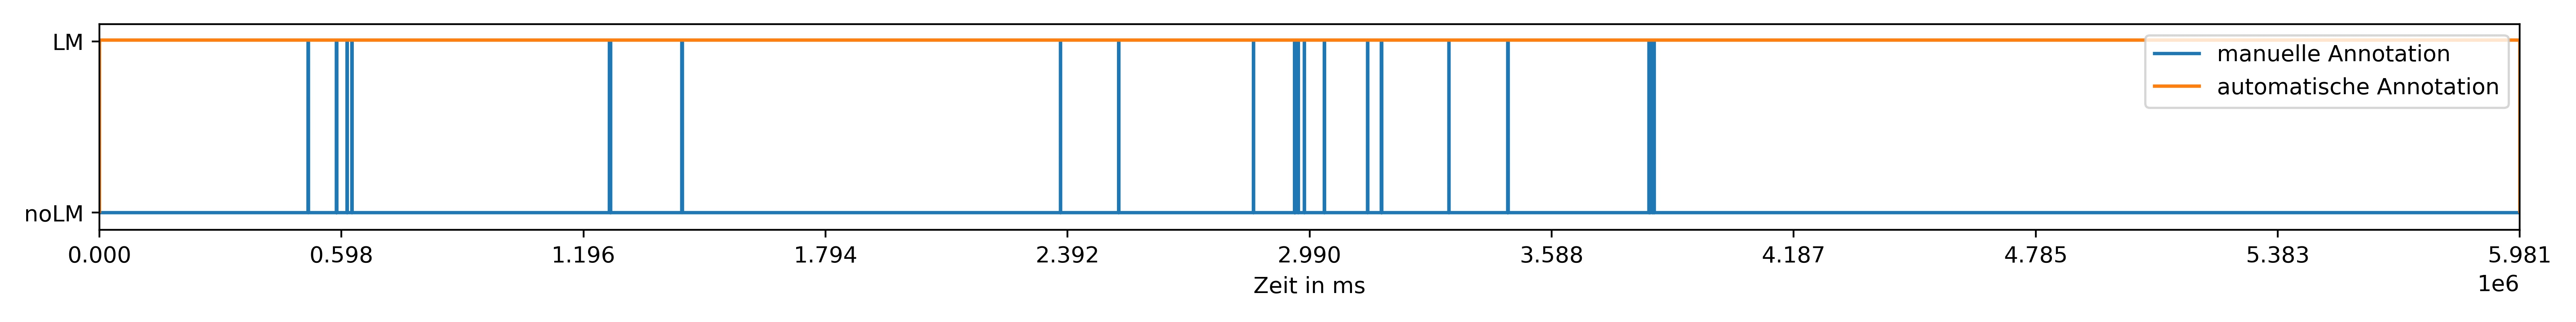
\includegraphics[width=0.80\textwidth]{./Bilder/customAll1.jpg}
	\end{center}
	\caption{Beispielannotation bei der die automatische Annotation nur positiv ist. Es entstehen Kosten von vier obwohl klassische Metriken Eins sind.}%
	\label{fig:all1}%
\end{figure}


In dem Beispiel \ref{fig:all0} wurde die automatische Annotation auf null gesetzt für die gesamte Nacht. Das Kostenfunktional kommt hier wieder auf einen Wert von 4 und auf relative Kosten von Eins. Die Genauigkeit und falsch positiv Rate sind in diesem Fall nicht definiert, da Zähler und Nenner Null sind. In diesem Fall werden die Metriken teilweise auch als Eins also als perfekte Genauigkeit definiert \cite{glassbox}. Laut Spezifität ist ein Detektor, der trivialerweise immer Null ausgibt also auch perfekt. 

\begin{figure}[!ht]%
	\begin{center}
	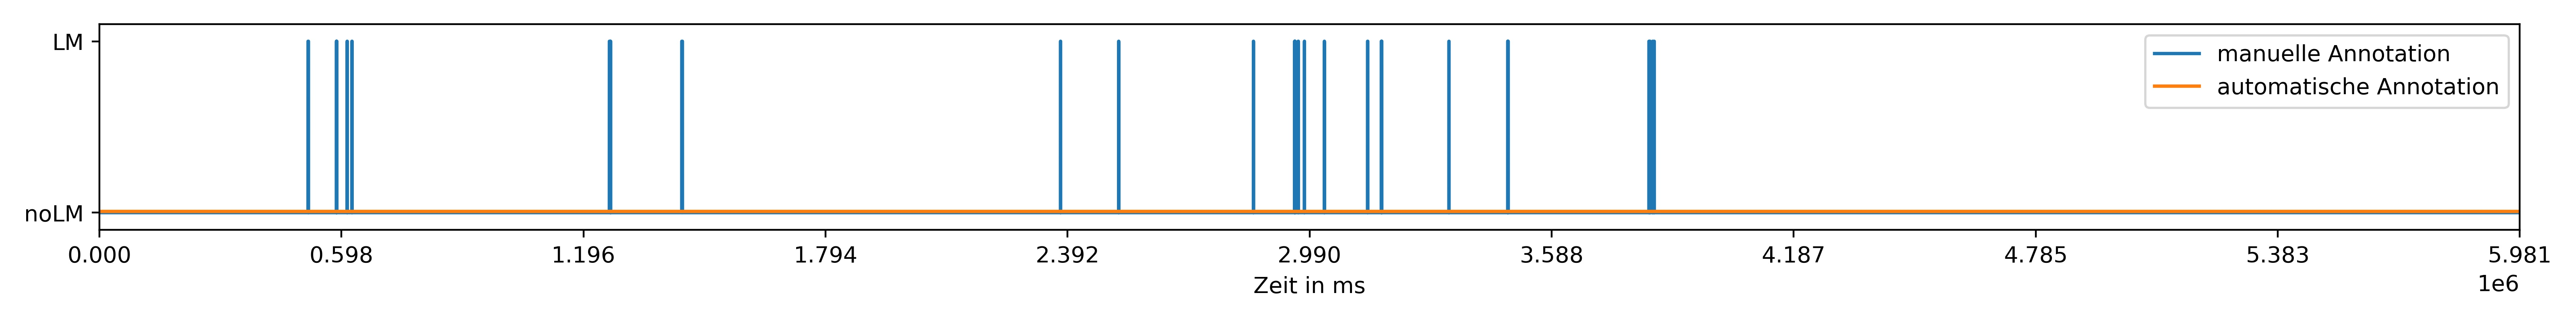
\includegraphics[width=0.80\textwidth]{./Bilder/AllZero.jpg}
	\end{center}
	\caption{Beispielannotation bei der die automatische Annotation nur negativ ist. Es entstehen Kosten von vier obwohl klassische Metriken Eins sind.}%
	\label{fig:all0}%
\end{figure}

Für einen Detektor, der die manuelle Annotation exakt nachbildet, wie in Bild \ref{fig:same} dargestellt, wären beide Annotationssignale identisch. Da hier keine Fehler gemacht werden sind die absoluten und relativen Kosten Null. Die Güte hat somit den perfekten Wert von Eins.

\begin{figure}[!ht]%
	\begin{center}
	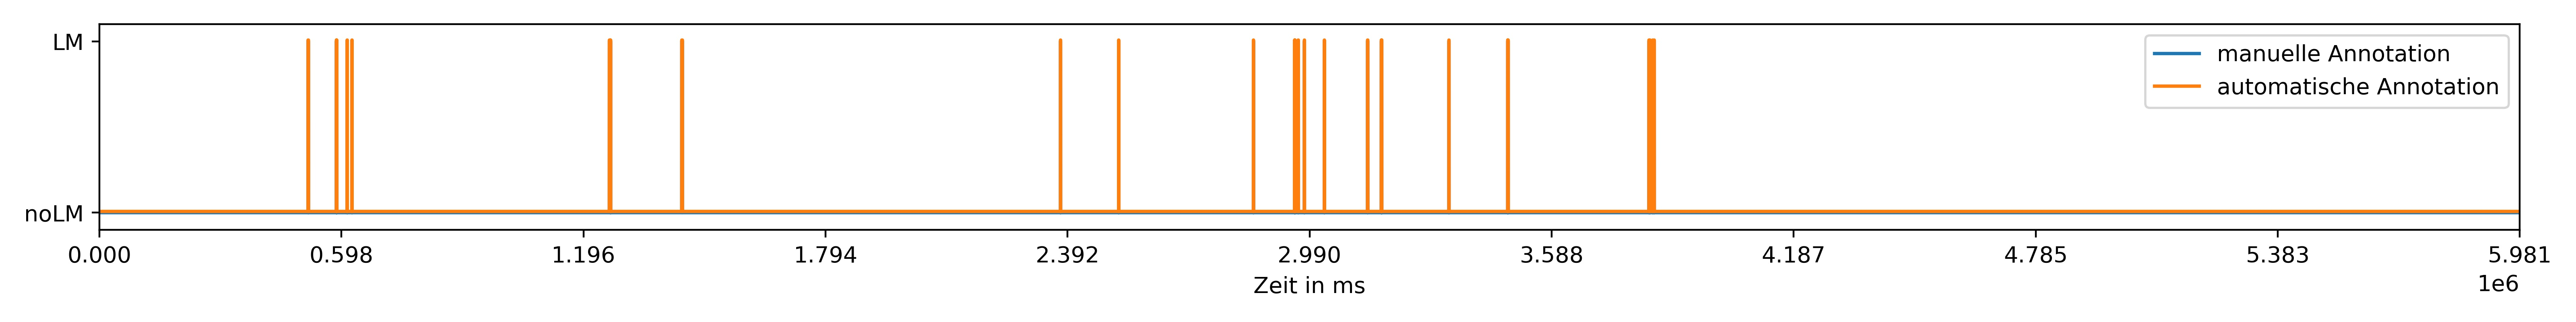
\includegraphics[width=0.80\textwidth]{./Bilder/aAnno=mAnno.jpg}
	\end{center}
	\caption{Beispielannotation bei der die automatische Annotation identisch zur manuellen Annotation ist. Die Güte des Detektors wäre in diesem Beispiel Eins.}%
	\label{fig:same}%
\end{figure}

Für die nachfolgenden Ergebnisse wurden Annotationssignale selbst erstellt, damit die einzelnen Kostenbeiträge besser veranschaulicht werden können.
Die Funktionsweise der multiplen Zuordnung lässt sich in Abbildung \ref{fig:Xto1} veranschaulichen. In dem Beispiel wurden der einen automatischen Annotation vier manuelle zugeordnet. Die absoluten Kosten sind wieder vier, da keins der vier manuell gefundenen PLM entdeckt wurde. Alle klassischen Metriken würden anhand dieses Signals einen perfekten Wert ausgeben. Das 1toX-Matching lässt sich analog darstellen. 

 
 \begin{figure}[!ht]%
	\begin{center}
	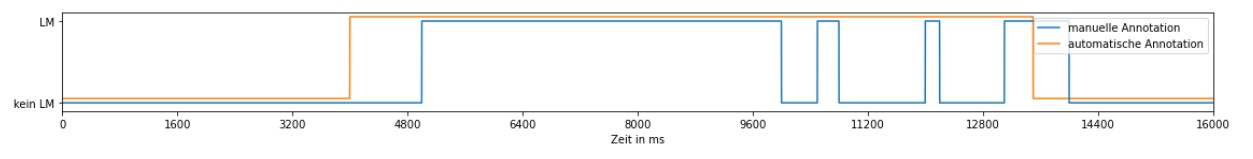
\includegraphics[width=0.80\textwidth]{./Bilder/Xto1.jpg}
	\end{center}
	\caption{Beispielannotation bei der die automatische Annotation einen Fehler durch Xto1-Matching aufweist.}%
	\label{fig:Xto1}%
\end{figure}

In Abbildung \ref{fig:FP} wird der Fehler aufgrund eines \gls{FP} dargestellt, welcher somit eine Serie feststellt, obwohl die manuelle Annotation keine PLM erkennt. Die Kosten sind hier ebenfalls vier.
\begin{figure}[!ht]%
	\begin{center}
	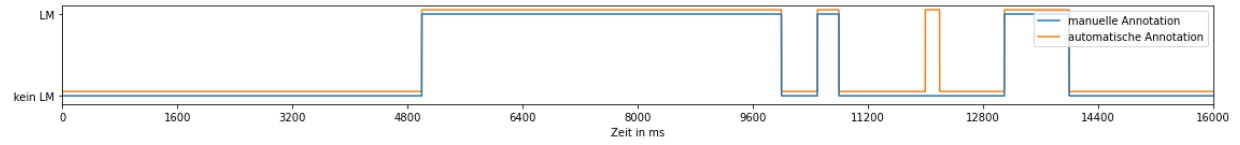
\includegraphics[width=0.80\textwidth]{./Bilder/FP.jpg}
	\end{center}
	\caption{Beispielannotation bei der die automatische Annotation einen Fehler aufgrund eines \gls{FP} aufweist.}%
	\label{fig:FP}%
\end{figure}

Die Abbildung \ref{fig:timevio} zeigt, dass eine zeitlich ungenaue Annotation in dem letzten LM ebenfalls zu einem Fehler führen kann. Hier erfüllt das LM der manuellen Annotation nicht die von der AASM geforderten Zeitbedingungen um als PLM zu zählen. 

\begin{figure}[!ht]%
	\begin{center}
	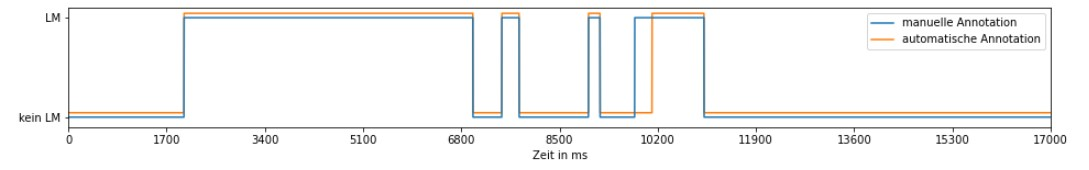
\includegraphics[width=0.80\textwidth]{./Bilder/TimeVio.jpg}
	\end{center}
	\caption{Beispielannotation bei der die automatische Annotation einen Fehler aufgrund eines ungenauen Startwertes aufweist.}%
	\label{fig:timevio}%
\end{figure}

In dem Beispiel \ref{fig:0.2Kost} wurde das letzte LM nicht erkannt und der Fehler aufgrund \gls{FN} beträgt Eins. Die relativen Kosten sind hier nur 0.2, da trotzdem vier der fünf LM in der PLM-Serie richtig erkannt wurden.


\begin{figure}[!ht]%
	\begin{center}
	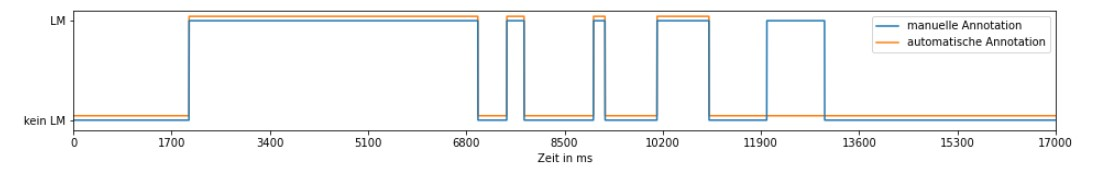
\includegraphics[width=0.80\textwidth]{./Bilder/0.2Kost.jpg}
	\end{center}
	\caption{Beispielannotation bei der die automatische Annotation einen Fehler aufgrund eines FN aufweist. Es entstehen relative Kosten von 0.2.}%
	\label{fig:0.2Kost}%
\end{figure}

Im Bild \ref{fig:achtKost} ist dargestellt, wie bei dem ersten automatisch erkannten LM ein Xto1-Matching vorliegt. Dieses wird aber gleichzeitig in eine weitere PLM-Serie aus FP gezählt. Obwohl die PLM Anzahl für beide Annotationen gleich ist, entstehen hier absolute Kosten von acht und relative Kosten von zwei. 

\begin{figure}[!ht]%
	\begin{center}
	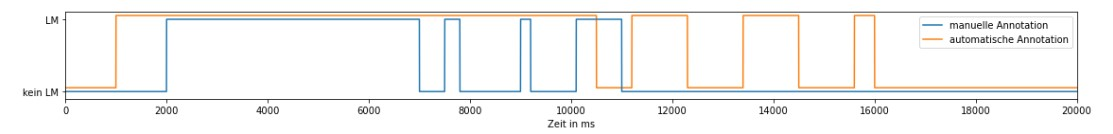
\includegraphics[width=0.80\textwidth]{./Bilder/underovercount.jpg}
	\end{center}
	\caption{Beispielannotation bei denen Kosten entstehen, obwohl die PLM Anzahl gleich ist. Es entstehen absolute Kosten von Acht.}%
	\label{fig:achtKost}%
\end{figure}




Falls es keine anderen außer die oben genannten Fehler gibt, müsste
\begin{equation}
\overset{\text{ergebniserhöhende Fehler \textminus \ ergebnisverkleinernde Fehler}}{\underset{\text{automatisch annotierte PLM \textminus \ manuell annotierte PLM}}{=}}
\label{kdiff}\end{equation}
gelten. Diese Gleichung beschreibt alle Fehler, die durch das Kostenfunktional gefunden werden können und setzt diese in Beziehung zu den tatsächlich auftretenden Fehlern. Mit dieser Gleichung kann also überprüft werden, ob alle einzeln gemachten Fehler auch gefunden wurden.

Es gibt jedoch auch Detektorfehler, die das Ergebnis nicht verändern aber trotzdem als Kosten zählen sollen. Zum Beispiel kann es passieren, dass eine manuell gefundene PLM Serie durch einen Zeitfehler (siehe Punkt 2) in zwar aus der einen Serie exkludiert wird, aber in einer anderen Serie damit inkludiert wird. 
Da sowohl Verkleinerung als auch Vergrößerung des Ergebnisses als falsch zu beurteilen ist, werden beide Fehlerarten addiert und bilden damit das Kostenfunktional: 
\begin{equation}
K_{abs} = ergebniserhöhende\ Fehler + ergebnisverkleinernde\  Fehler     
\end{equation}

Die absolute Anzahl an Fehlern kann bei unterschiedlichen Datensätzen irreführend sein, da zwar die Wahrscheinlichkeit einen Fehler zu machen gleich sein sollte, aber bei mehr Events auch mehr Fehler entstehen. Daher sollte das Kostenfunktional auf die Anzahl der manuell annotierten PLM in der jeweiligen Serie normiert werden. Somit sind die Kosten auch unabhängig von der durchschnittlichen Länge der PLM-Serien. Das finale Kostenfunktional stellt also dar wie viele Fehler pro richtig erkannte PLM gemacht werden.


\section{Verbesserung der Einordnung des Detektors}\label{Verbesserung}


Dieses Kapitel bezieht sich darauf weitere nützliche Information aus den Annotationssignalen zu extrahieren, um mit diesen den Detektor besser einschätzen zu können. Diese Metriken gehen nicht in die Berechnung der Güte ein, können aber informativ genutzt werden.

Da sich die anderen Metriken hauptsächlich auf einzelne LM beziehen, könnte eine Metrik nützlich sein, welche große Veränderungen der Annotationen im Laufe der Nacht, darstellt. Diese könnte durch den Schwerpunkt der Startzeitpunkte der LM berechnet werden. Da das Gewicht jedes LM eins ist, und der Abstand gleich des Startzeitpunktes ist, geht die Berechnung des Schwerpunktes in die des Mittelwertes über.
Dieser Wert könnte dafür genutzt werden, große Veränderungen, bei denen sich die Annotation im Laufe der Nacht ändert, zu erkennen. Interessant ist auch, ob diese Veränderung von beiden Annotationen gleichermaßen detektiert wurde. Also berechnet sich die Metrik aus der Differenz der beiden Schwerpunkte.

Eine weitere Information steck in der zeitlichen Genauigkeit der Start- und Endzeitpunkte der Beinbewegungen. Diese lassen sich nur bei der eventweisen Zuordnung von Beinbewegungen zu TP analysieren. 
Falls eines der beiden Annotationssignale segmentweise ausgewertet wurde, geht genauere Information zu den Startzeitpunkten verloren. Diese Genauigkeit könnte in dem anderen Annotationssignal höher sein. Betrachtet man nun die Differenz der jeweiligen Startzeitpunkte von TP entsteht eine Verteilung. Die nächsten beiden Metriken beschreiben also den Mittelwert und die Standardabweichung dieser Verteilung. Da die Wahrscheinlichkeit des zeitlich höher aufgelösten Annotationssignal ein LM-Start zu haben unabhängig von den Segmentgrenzen des andren Annotationssignals ist, liegt der Erwartungswert bei null.
Analog lässt sich auch eine Verteilung für die Endzeitpunkte der LM berechnen.

Eine hohe Anzahl an FP in einzelnen Nächten könnte darauf hindeuten, dass Events manuell entweder nicht betrachtet wurden oder nach einer Annotation im Nachhinein wieder gelöscht wurden. Die klassische Metrik der falsch positiv Rate könnte ein Indiz über diese Art von Uneinigkeit geben.

Des Weiteren lassen sich Information gewinnen, welche genutzt werden kann, um die Arbeitsweise des Detektors besser zu verstehen, um den Detektor gegebenenfalls zu optimieren.
So kann beispielsweise das Verhältnis aus der Anzahl automatisch gefundener LM zu der Anzahl manuell gefundener LM darauf hindeuten wie schnell der Detektor auf positive Änderungen im EMG reagiert. 


Eine Verwandte Information liefert die Anzahl der multiplen Zuordnung (Xto1- und 1toX-Matching). Diese Werte könnten beschreiben wie schnell der Detektor auf eine negative Änderung im EMG reagiert. 

Da Beinbewegungen laut AASM eine bestimmte Mindest- und Maximaldauer haben, könnte die Zahl der Verstöße gegen diese Zeiten aufschlussreich über die Art der gefundenen Muskelkontraktionen. 

Diese Informationen sind allerdings nur im Kontext der Funktionsweise des Detektors nützlich und sollten nicht zur Bewertung verwendet werden.

In der Grafik \ref{fig:Metriken} sind die nützlichen Informationen zum Detektor dargestellt. Der obere Kreis bezieht sich auf den Vergleich zu bisherigen Detektoren. Hierfür sind die angegebenen klassischen Metriken am nützlichsten, da diese von den bisher entwickelten Detektoren angegeben wurden. Diese können außerdem einen guten Überblick darüber geben, wie viele von den Beinbewegungen circa richtig erkannt werden. Besonders Cohens $\kappa$ und das F1-Maß treffen eine vergleichsweise genaue Aussage.
Links im Bild sind die Informationen zu dem Detektor dargestellt, welche Aussagen über die Funktionsweise des Detektors liefern.
Der rechte Unterpunkt beschreibt das Kostenfunktional und seine Einflussfaktoren.
\begin{figure}[!ht]%
	\begin{center}
	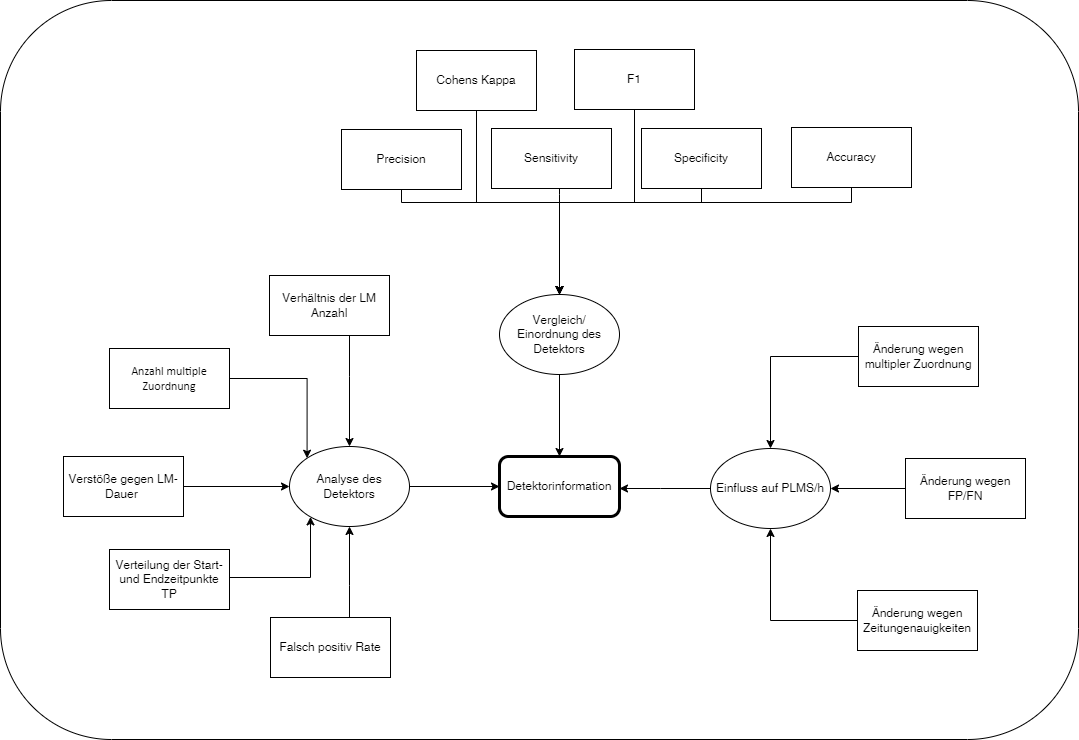
\includegraphics[width=0.80\textwidth]{./Bilder/Metrik.png}
	\end{center}
	\caption{Darstellung der Metriken, die zum Informationsgewinn oder zur Bewertung des Detektors verwendet werden können.}%
	\label{fig:Metriken}%
\end{figure} \newpage
\chapter{Anwendung der Metriken}\label{chap:Anwendung_der_Metriken}
\section{Datensatz}\label{chap:Datensatz}
Der Datensatz, auf dem der Detektor ausgewertet werden soll, wurde im Uniklinikum Dresden  unter Verwendung des Alice System der Version 5 von Phillips erhoben. Für die Auswertung der EMG-Signale wurden die Kriterien der AASM angewendet und die Annotationsunterstützung des Alice Systems genutzt. 

Es wurde ein Hochpassfilter mit einer Grenzfrequenz von 10 Hz und ein Tiefpassfilter mit einer Knickfequenz von 93.6 Hz verwendet. Zusätzlich kam ein 50 Hz Notchfilter zur Anwendung. Die Abtastfrequenz beträgt 200 Hz.

Beim Bearbeiten des Datensatzes wurden 296 Dateien ohne manuelle Annotation gefunden und ausgeschlossen. 
Bei weiteren 12 Dateien wurde der gleitende Mittelwert nicht richtig berechnet. Dieser Fehler entsteht, wenn das vom Detektor erkannte Hintergrundrauschen $\eta(n)$ 50 $\mu V$ überschreitet. Der Algorithmus setzt in diesem Fall den oberen Schwellwert richtigerweise auf unendlich. Bei Benutzung der Bibliothek scilab entstehen bei der Faltung jedoch ungültige Werte, welche nicht für die weitere Berechnung verwendet werden können. Der Fehler konnte anhand einiger Beispiele nachvollzogen werden und es wird davon ausgegangen, dass bei allen 12 Dateien das gleiche Problem vorlag.
Die Ergebnisse basieren somit auf 5908 von ursprünglich 6216 Dateien im EDF-Format.


Es wurden von 3025 Personen das Alter und das Geschlecht aufgenommen. Das Geschlechtsverhältnis (M/F) beträgt 1.48 und die Alterszusammensetzung ist in Abbildung \ref{fig:Altershist} dargestellt.
\begin{figure}[!ht]%
	\begin{center}
	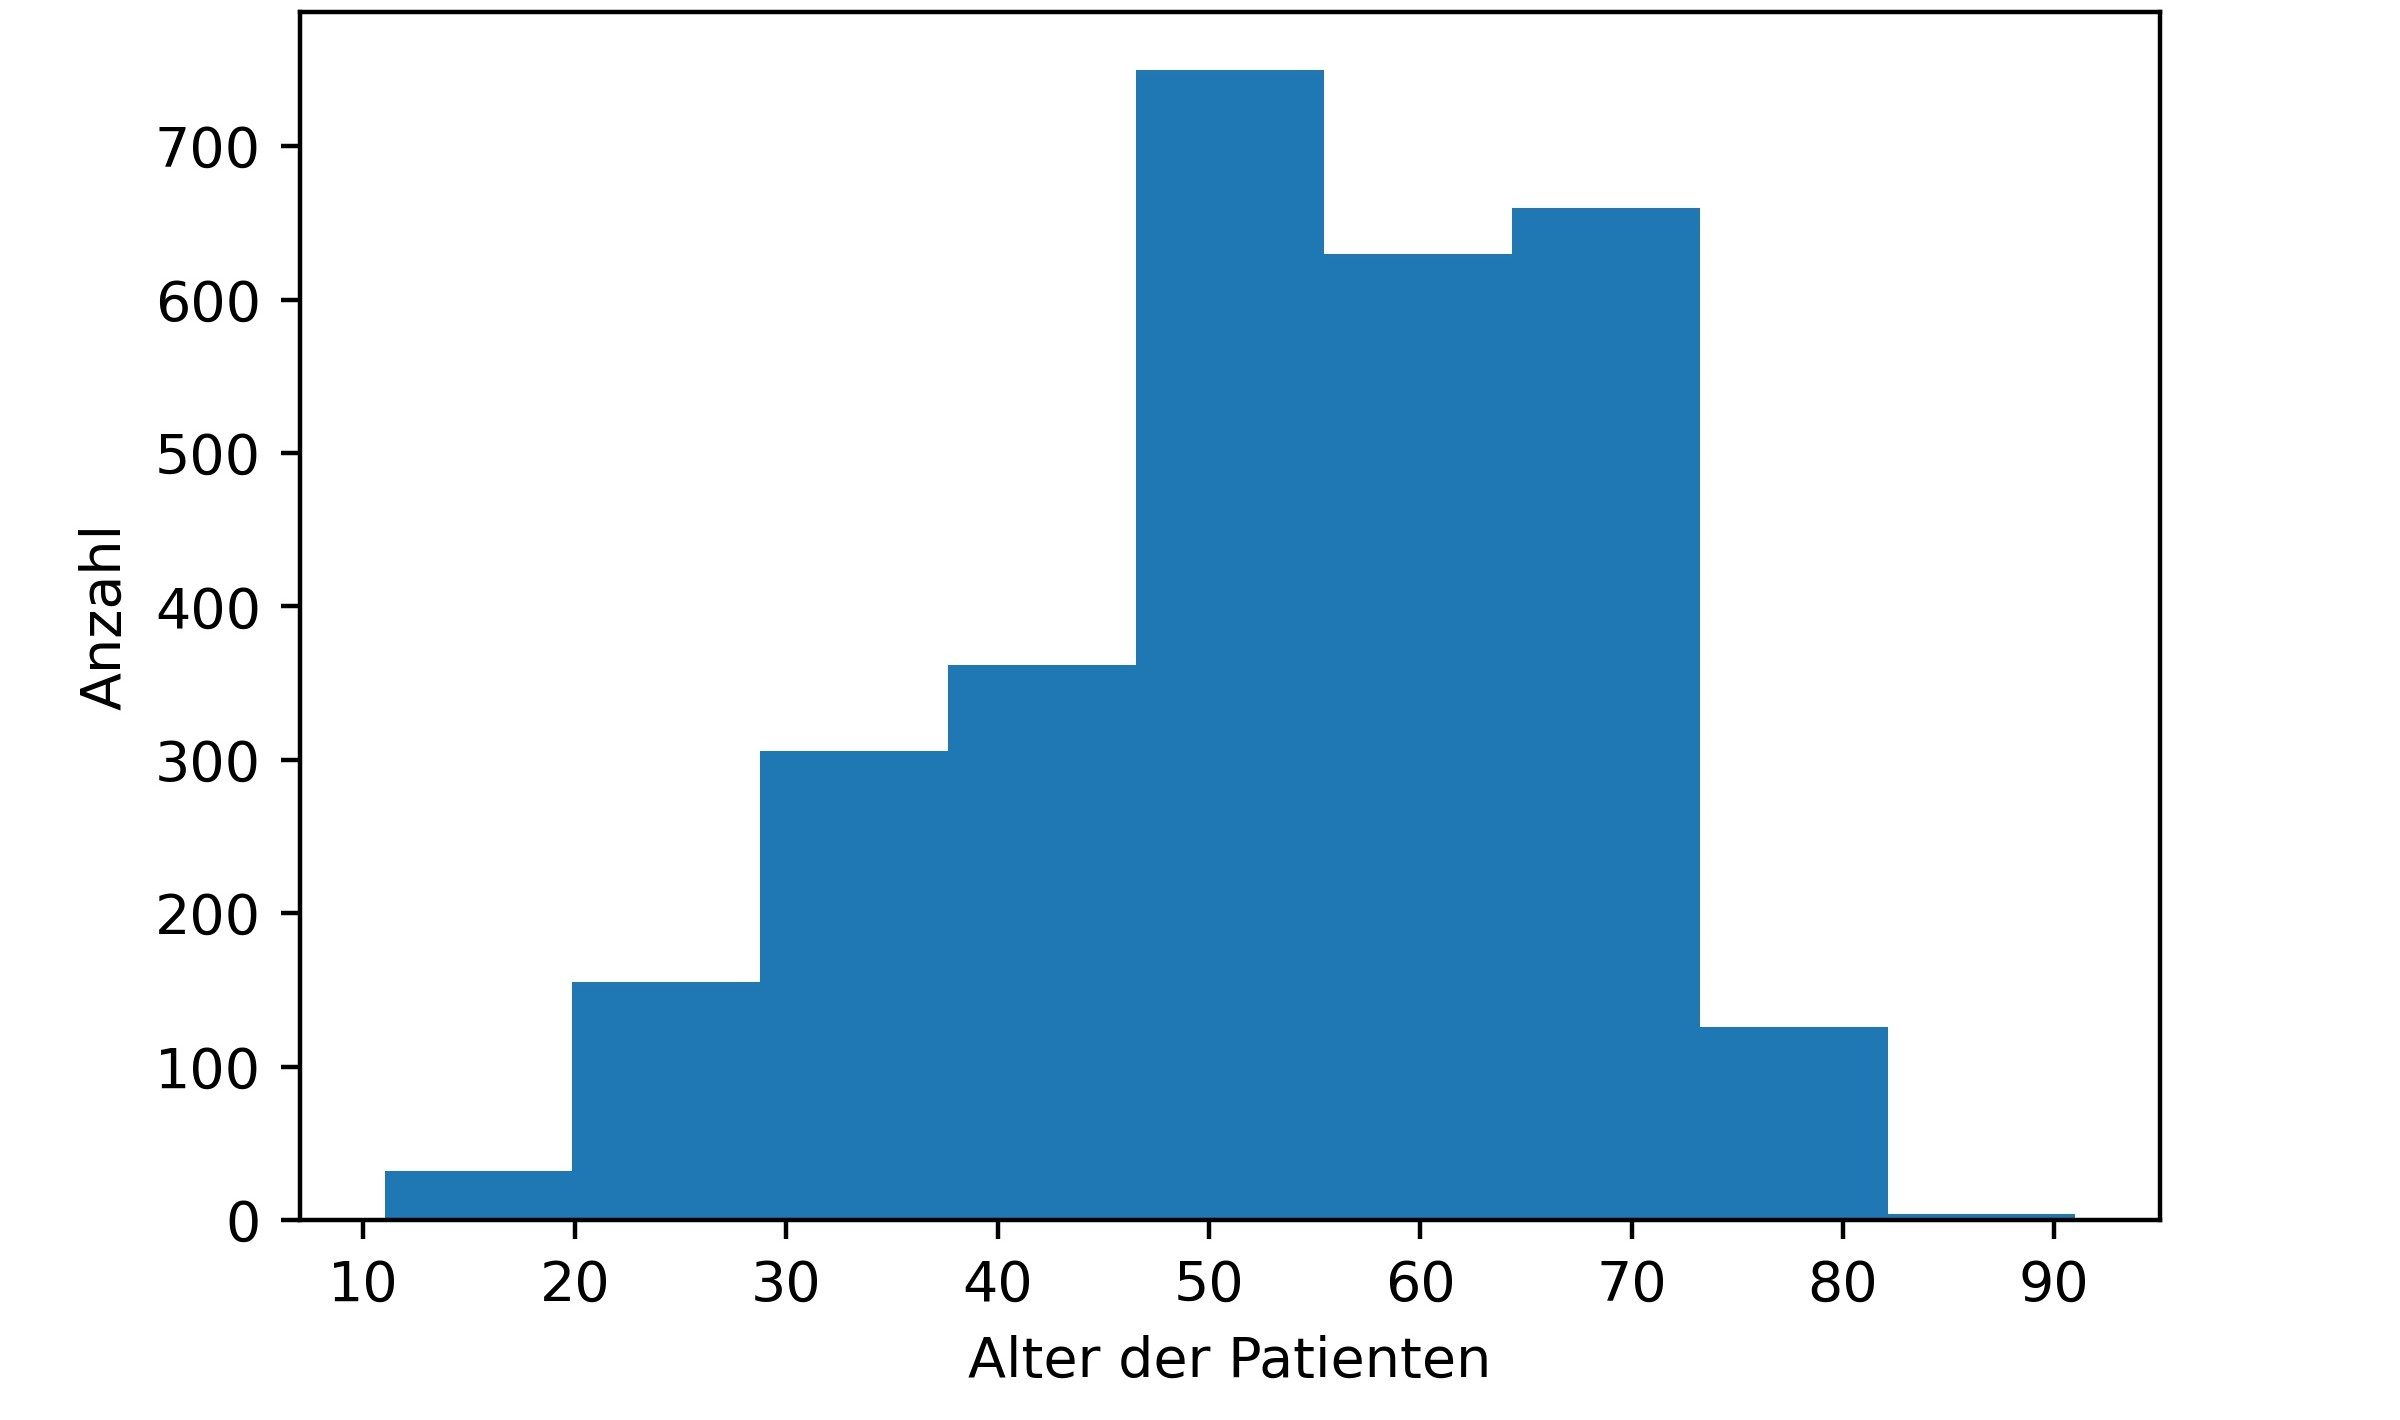
\includegraphics[width=0.80\textwidth]{./Bilder/MetadataAltershistogramm.jpg}
	\end{center}
	\caption{Histogramm der Demographie des Datensatzes.}%
	\label{fig:Altershist}%
\end{figure}

Die manuelle Annotation ist in 0.5 Sekunden Segmente unterteilt. Die Analyse der manuellen Annotationen ergibt eine durchschnittliche Anzahl von LM im Schlaf von 266. Am häufigsten aufgetreten sind Aufzeichnungen mit 17 annotierten LM. Der durchschnittliche PLMS/h-Wert liegt bei $9.95 * 10^{-3}$. Dabei haben 875 Dateien einen Wert von Null.

\section{Wahl des Detektors}\label{chap:WahldesDetektors}
Um die gefundenen Metriken anzuwenden, soll für diese Arbeit ein Detektor umgesetzt werden. 
Augenscheinlich sind die vorgeschlagenen Detektoren in der Tabelle im Stand der Technik ausreichend performant, sodass hier auf die Entwicklung eines neuen Detektors verzichtet werden kann.
Die am weitesten verbreitete Methode – und somit auch am weitesten entwickelte Methode – nutzt eine EMG-Signalvorverarbeitung und einen doppelten Schwellwertvergleich mit Nachbearbeitung des Annotationssignals. Der Vorteil eines Schwellwertvergleiches liegt außerdem in einer geringen Rechenlaufzeit, da keine Modelle trainiert werden müssen und die Berechnungen leicht zu parallelisieren sind. 
Der Algorithmus von Huang et al. wurde nur auf einem sehr kleinen Datensatz getestet und benötigt eine hohe EMG-Qualität, da ein absoluter Schwellwert implementiert ist. Die Variante von Moore baut auf den Erkenntnissen von Ferri et al., Tauchmann und Wetter et al. auf. 

Also wurde für den Rahmen dieser Arbeit der Detektor von Moore et al. implementiert. Es gibt zwar eine weiterentwickelte Variante von Alvarez-Estevez, welche bessere Ergebnisse liefert, diese ist jedoch wesentlich komplizierter aufgebaut und schwieriger vergleichbar mit den anderen Detektoren, da die Metriken anhand von einsekündigen Segmenten erstellt wurden. 
Da es in dieser Arbeit hauptsächlich um die Untersuchung der Metriken geht, ist die von Moore et al. erreicht Klassifikationsgüte ausreichend. 

Die Funktionsstruktur des Programms wurde im Stand der Technik beschrieben und ist hier in Python implementiert. Deswegen werden hier nur die Anpassungen beschrieben:
Beim Einlesen der Dateien werden die leeren Annotationssignale übersprungen, da diese keinen Informationsgehalt bieten. Die beiden EMG-Signale der Beine werden laut \cite{Moore} zu einem Signal zusammengeführt. Die Signale für beide Beine einzeln zu berechnen wie in \cite{alvarez} funktioniert hier nicht, da für die Nachbearbeitung der Annotationssignale ein Grundrauschen des kombinierten Signals gebraucht wird.
Das RMS-Signal und der gleitende Mittelwert werden mit einer Randeffektanpassung errechnet, um das Signal nicht an den Rändern zu verfälschen. 
Hierbei werden die erkannten LM gelöscht, welche vor dem „Licht aus“-Zeitpunkt und nach „Licht An“-Zeitpunkt stattgefunden haben, da diese auch nicht in dem manuellen Annotationssignal vorhanden sind. 
Es werden auch Beinbewegungen entfernt, welche laut AASM die Maximallänge von 10 Sekunden überschreiten. Durch das Zusammenführen der beiden Beine dürfen laut AASM alternierende Bewegungen zusammengefasst werden. Mit zusätzlicher Filterung sind Beinbewegungen im Signal von mehr als 15 Sekunden möglich. Für bessere Vergleichbarkeit mit der Literatur wurde der Wert aus der Arbeit von Moore et al. implementiert. 

Bei der Umsetzung des Detektors wurde die adaptive Filterung der Elektrokardiogrammstörung und die Löschung der Beinbewegungen in der Nähe von atembezogenen Events verzichtet, da die benötigten Signale nicht zur Verfügung gestellt wurden. 

Die automatischen und manuellen Annotationen werden mit den jeweiligen Start- und Endzeitpunkten in einer CSV-Datei gespeichert.
Ein separates Programm kann die Annotationssignale aus den CSV-Dateien auslesen und daraus die Metriken bestimmen. Hier wird auch das Signal zu den Schlafstadien geladen, um die LM zu entfernen, die nicht im Schlaf stattgefunden haben. 
Des Weiteren gibt es ein Programm, welches alle pro Nacht berechneten Metriken einliest und zwischen den Nächten vergleicht.

\section{Funktion des Detektors}
An folgendem Beispiel lässt sich gut die Funktionsweise des Detektors anhand des Schwellwertes und die folgende Nachbearbeitung nachvollziehen. In Abbildung \ref{fig:detectorWorking2} ist oben das vorbearbeitete EMG-Signals (blau) und der davon abhängige dynamische obere Schwellwert zu erkennen. In dem Annotationssignal darunter ist ein Zwischenergebnis des Detektors zu sehen, bei dem alle Zeiträume annotiert wurden, bei denen das EMG-Signal über dem Schwellwert liegt. 
Das unterste Bild zeigt das finale automatische (orange) Annotationssignal nach der Nachbearbeitung. Dazu ist die manuelle Annotation zum Vergleich in blau auf der gleichen Achse dargestellt. 



\begin{figure}[!ht]%
	\begin{center}
	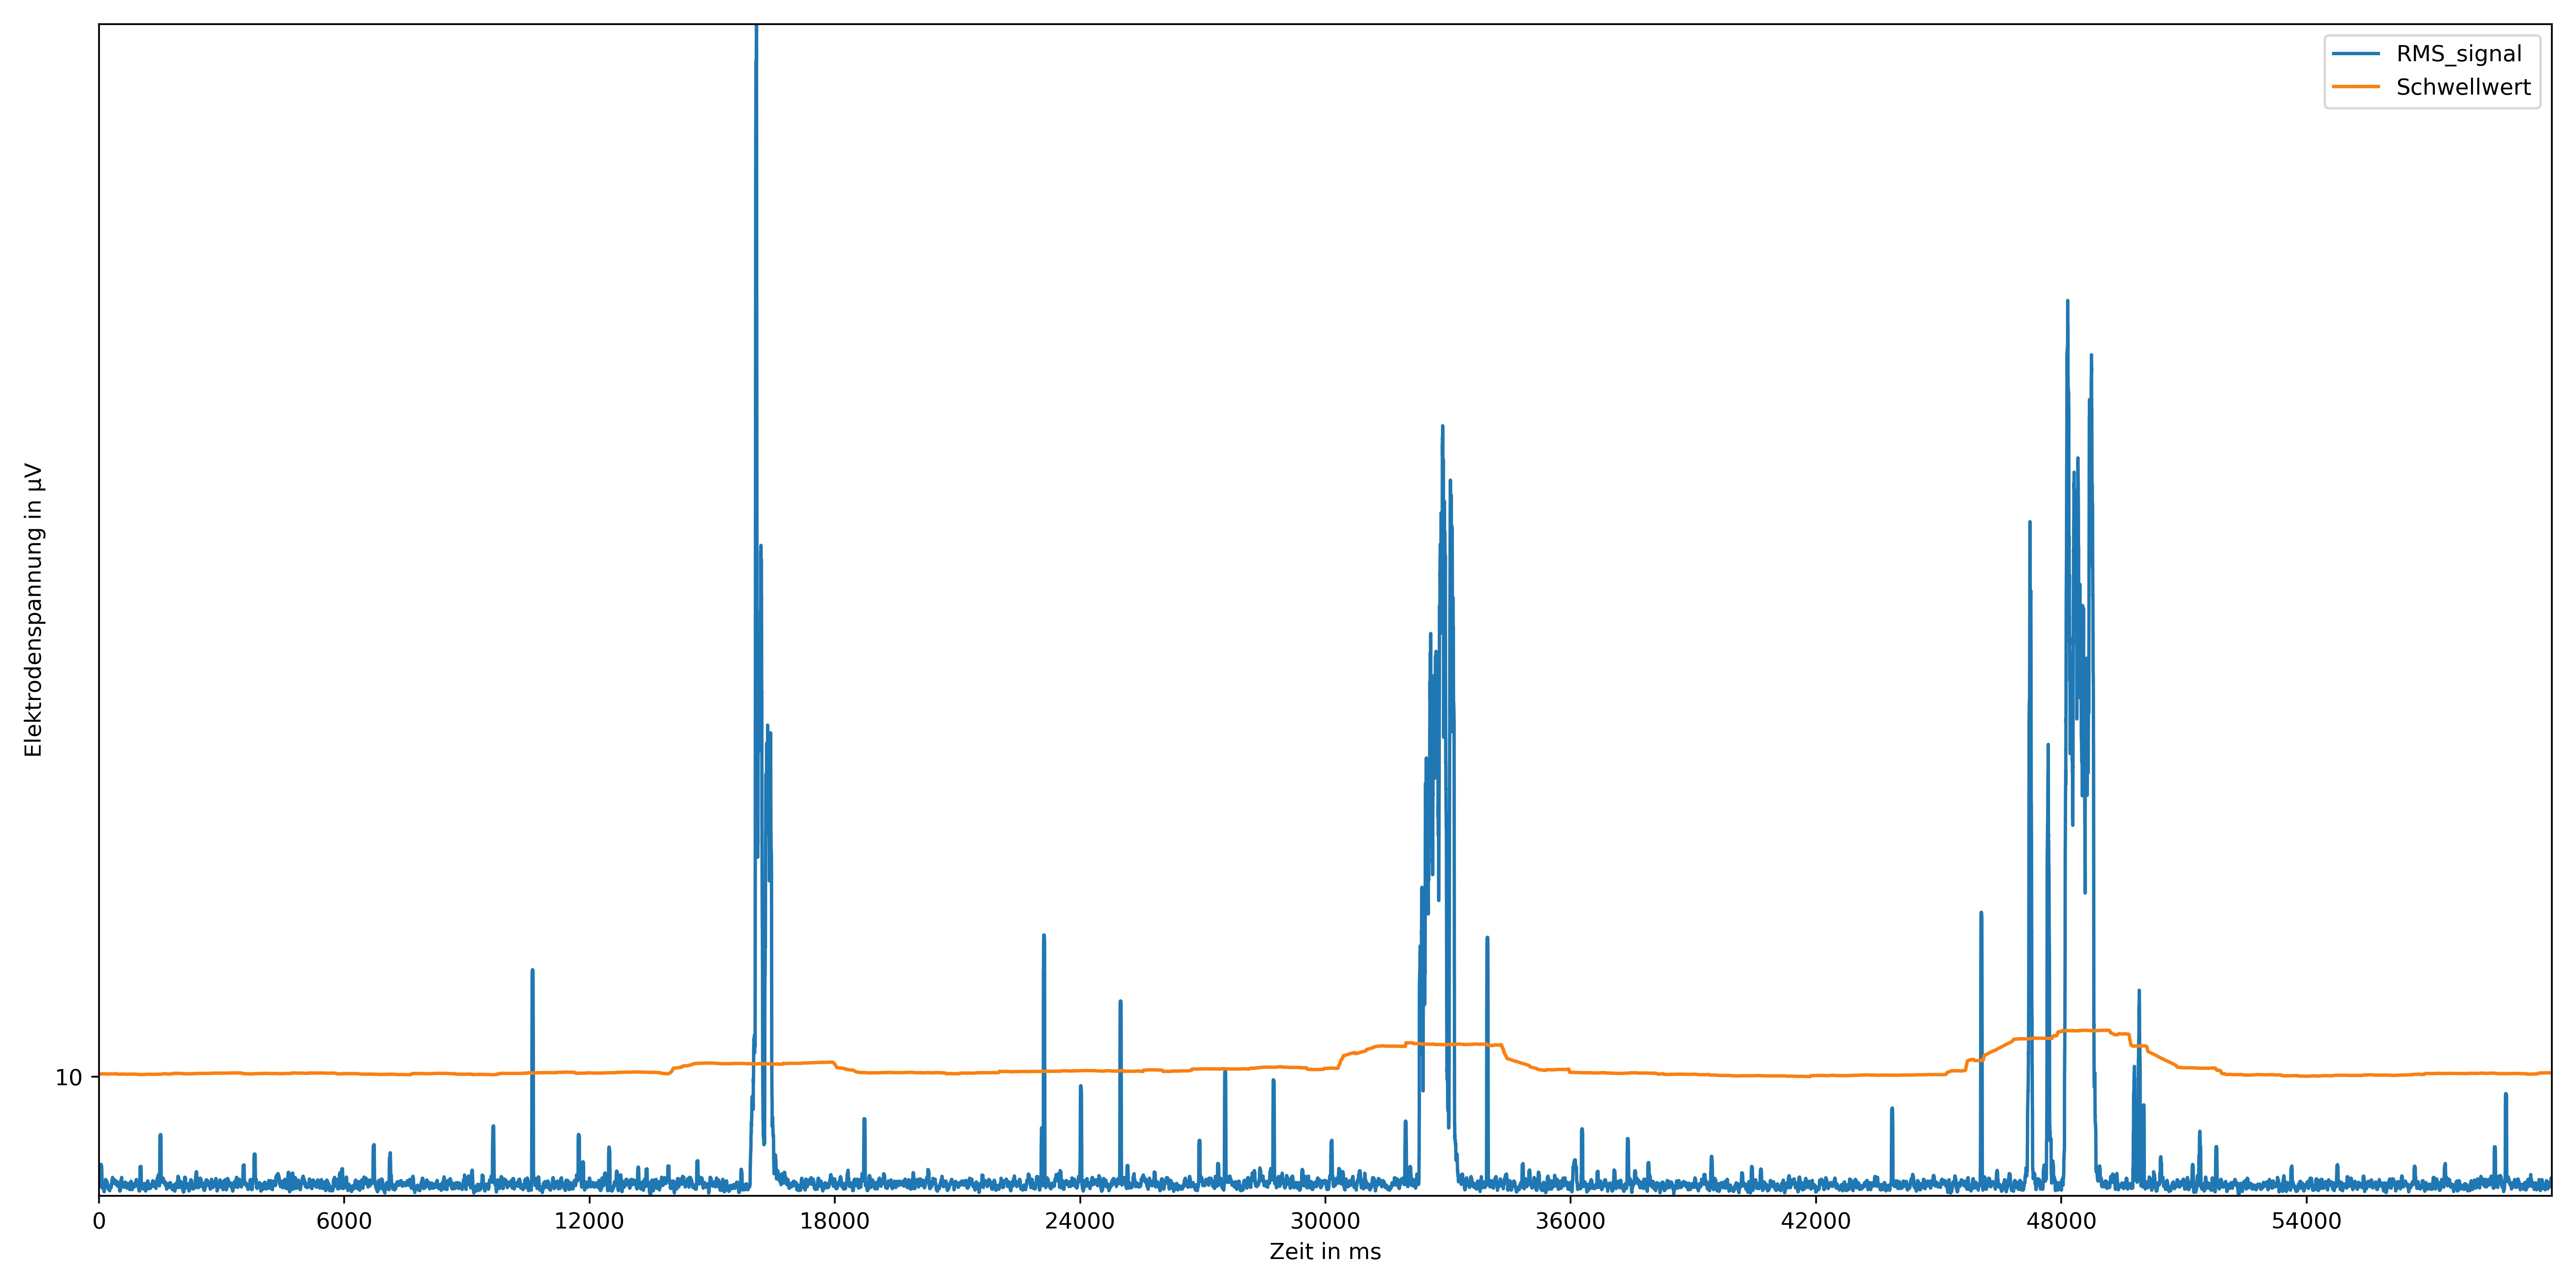
\includegraphics[width=0.80\textwidth]{./Bilder/detectorWorkEMGacq_002944221.edf2870000,60000.jpg}
	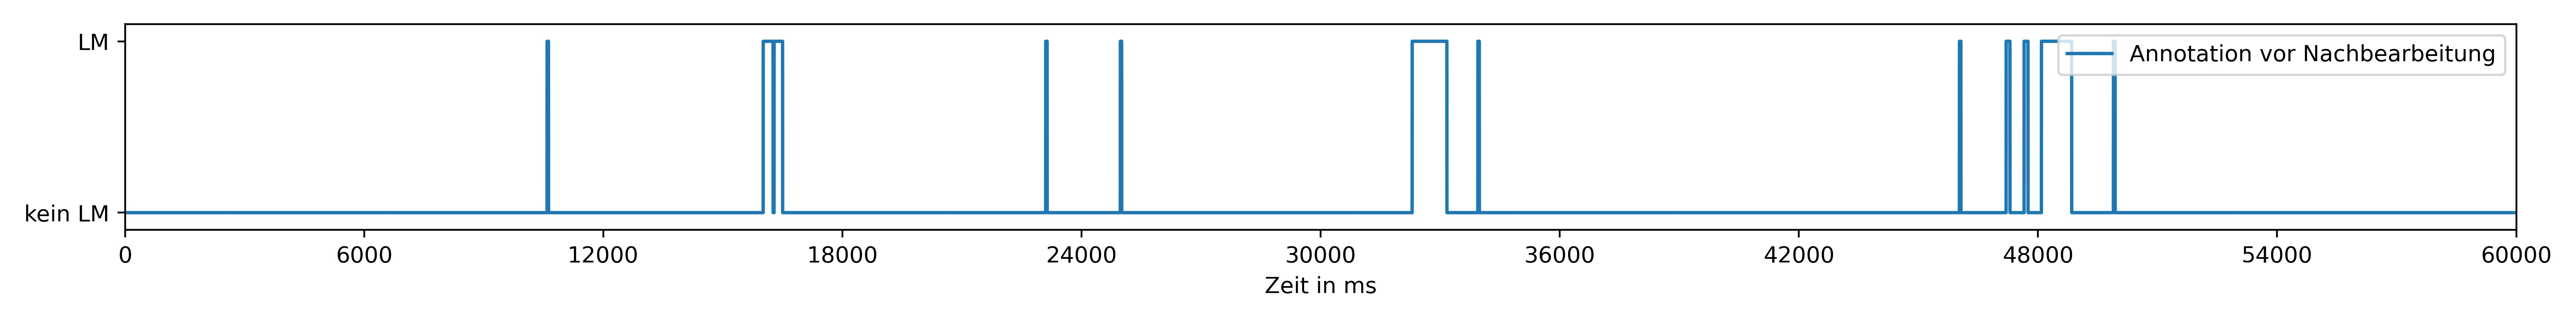
\includegraphics[width=0.80\textwidth]{./Bilder/detectorWork2acq_002944221.edf2870000,60000.jpg}
	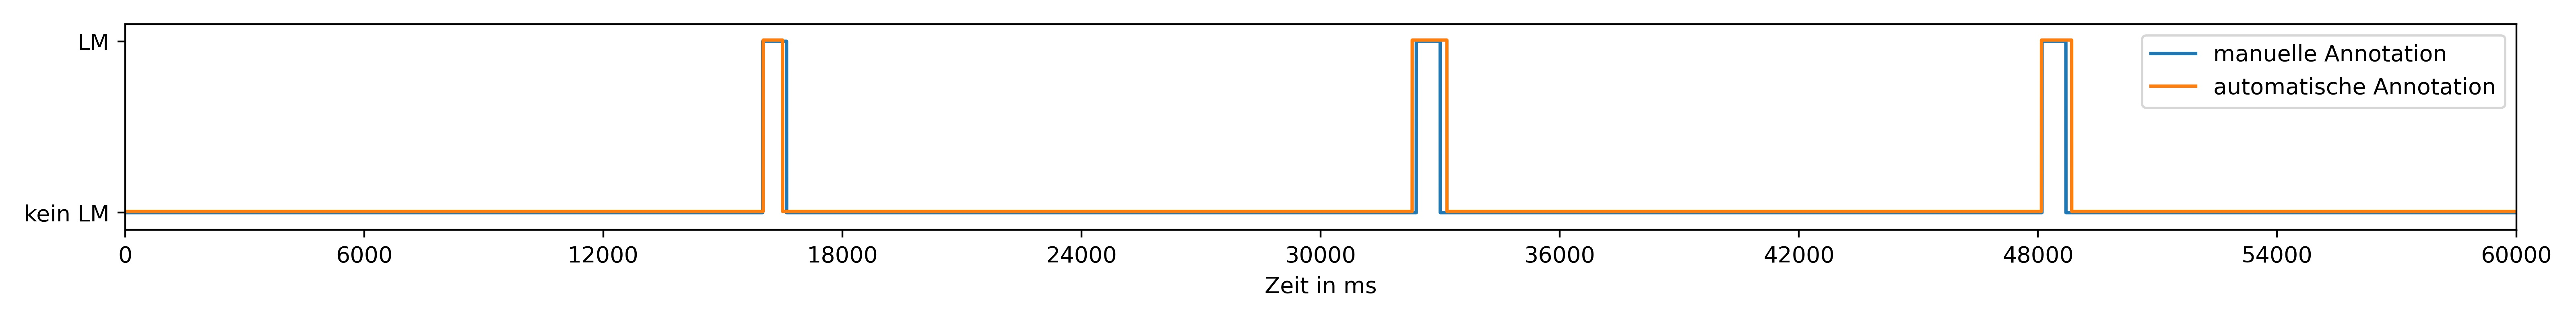
\includegraphics[width=0.80\textwidth]{./Bilder/detectorWorkacq_002944221.edf2870000,60000.jpg}
	\end{center}
	\caption{Veranschaulichung der Funktionsweise des implementierten Detektors: vorverarbeitetes EMG-Signal mit oberem Schwellwert (oben), Zwischenergebnis des Annotationssignals vor der Nachbearbeitung (mittig), finale automatische und manuelle Annotation zum Vergleich (unten). Die Abtastfrequenz beträgt 200 Hz.}%
	\label{fig:detectorWorking2}%
\end{figure}

Damit bei unregelmäßigem EMG-Signal keine \glspl{LM} erkannt werden, passt sich der dynamische Schwellwert an die veränderte Qualität an. 
In Abbildung \ref{fig:detectorWorking} lässt sich der Vorteil eines dynamischen Schwellwertes veranschaulichen. Für den dargestellten Zeitraum wurden manuell keine Beinbewegungen annotiert.

\begin{figure}[!ht]%
	\begin{center}
	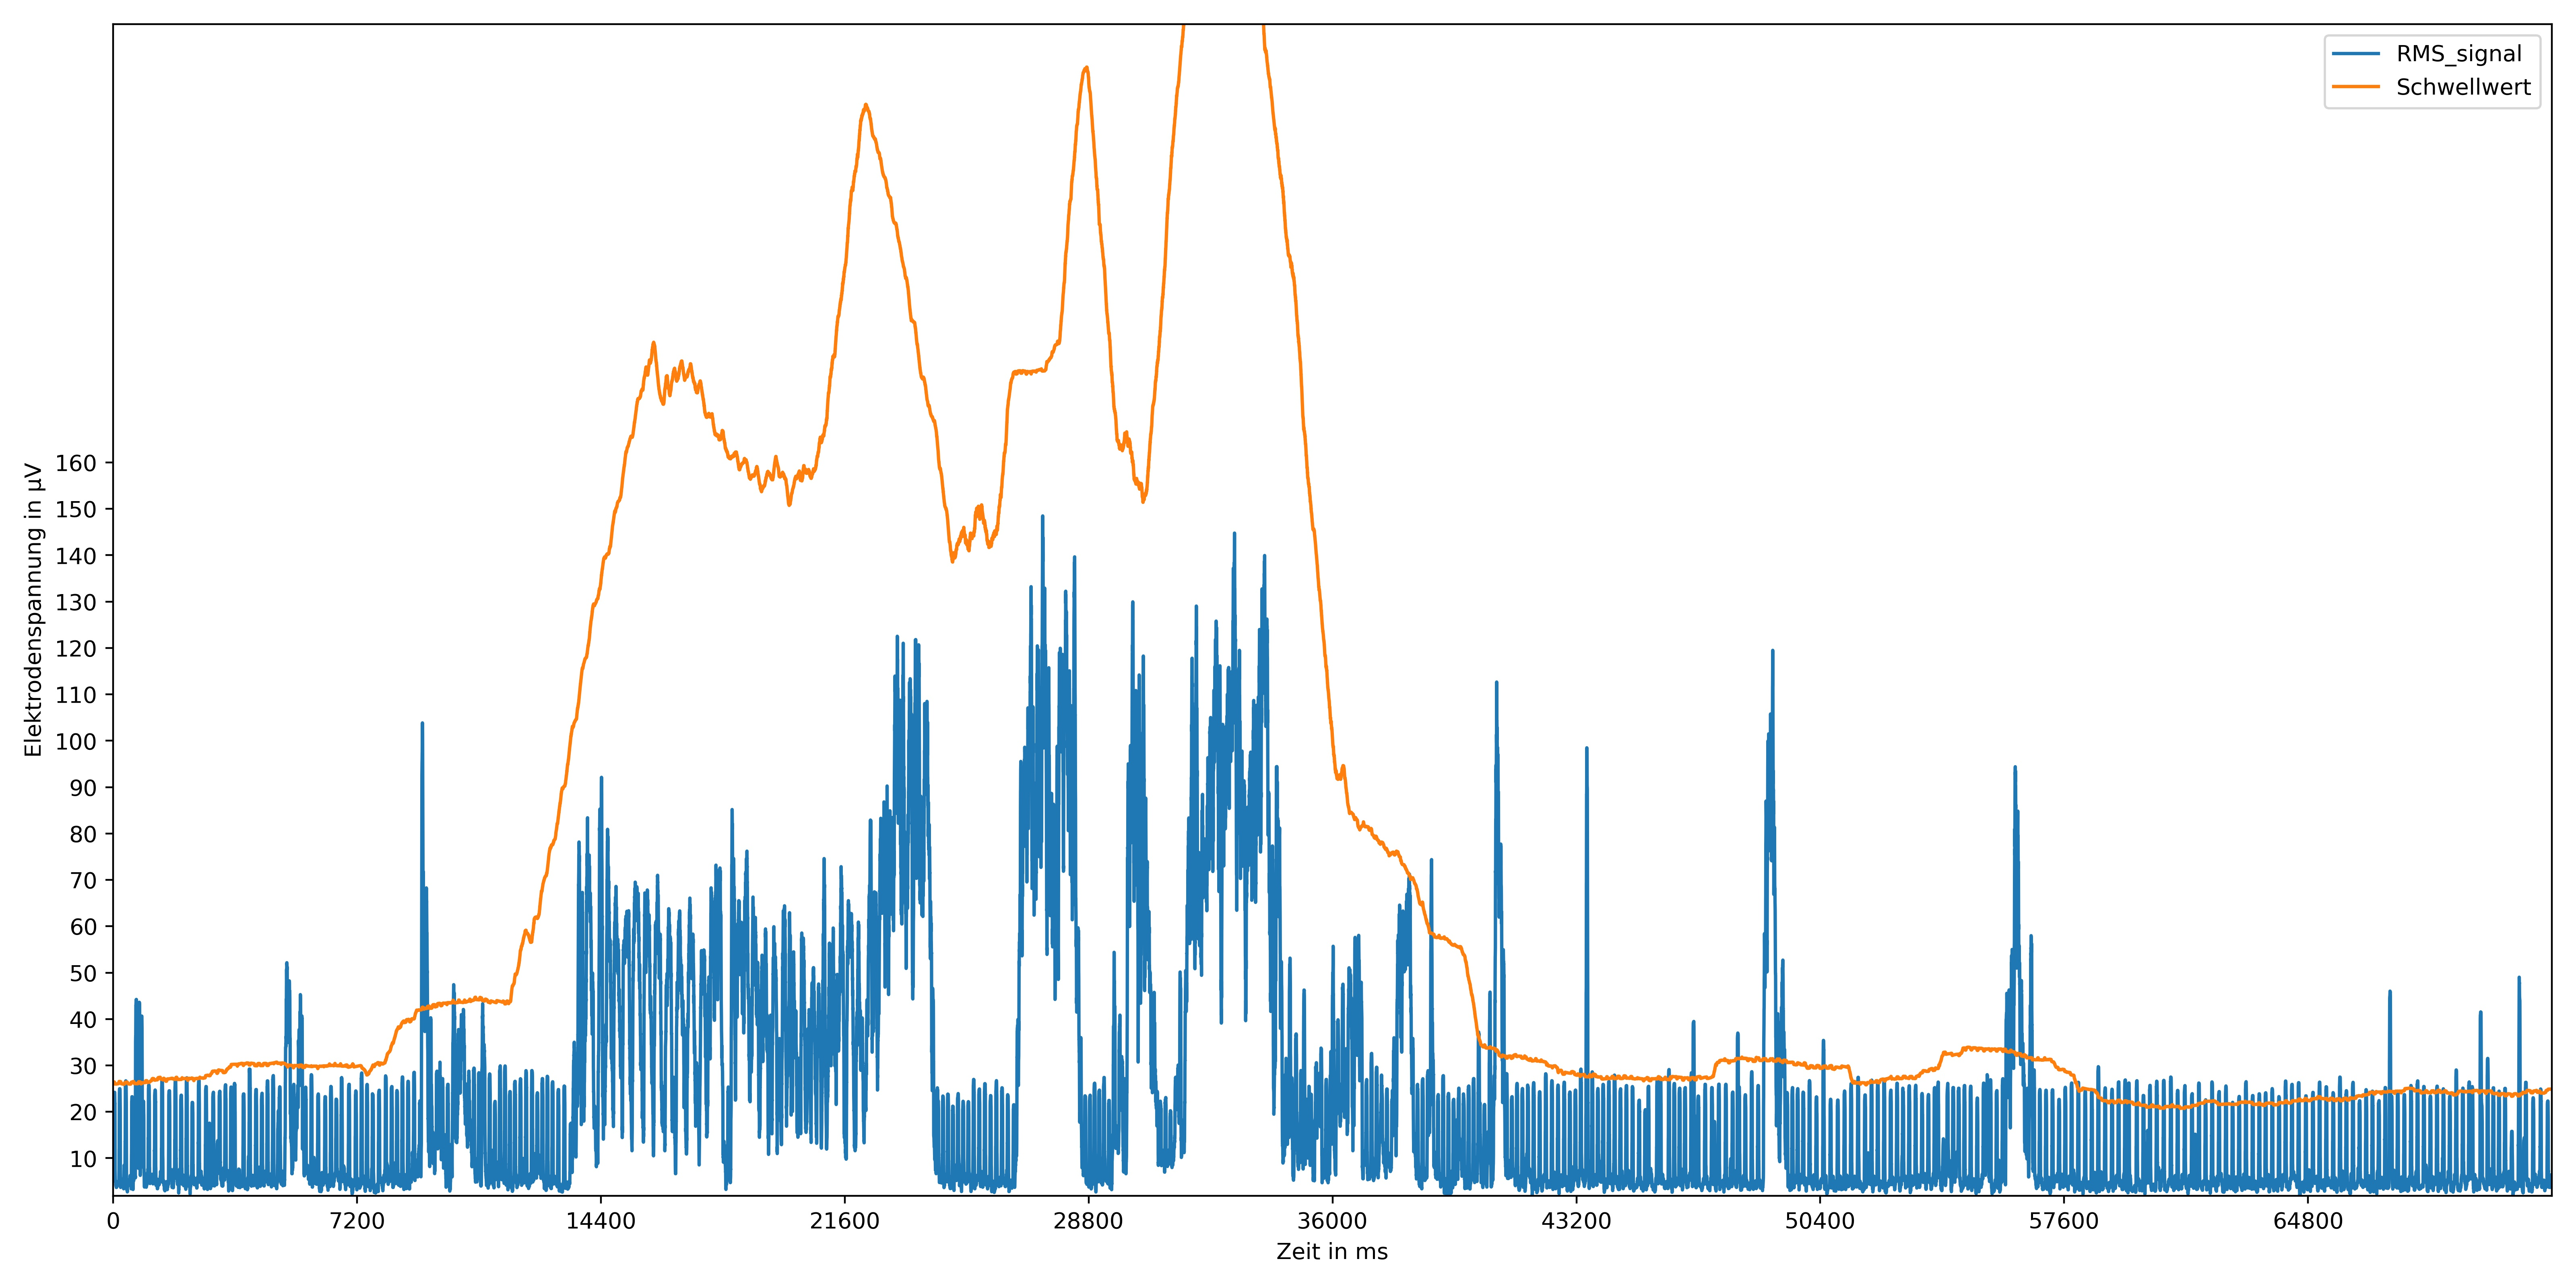
\includegraphics[width=0.80\textwidth]{./Bilder/vorrübergehendesRauschenEMGacq_002963603.edf108000,72000.jpg}
	
	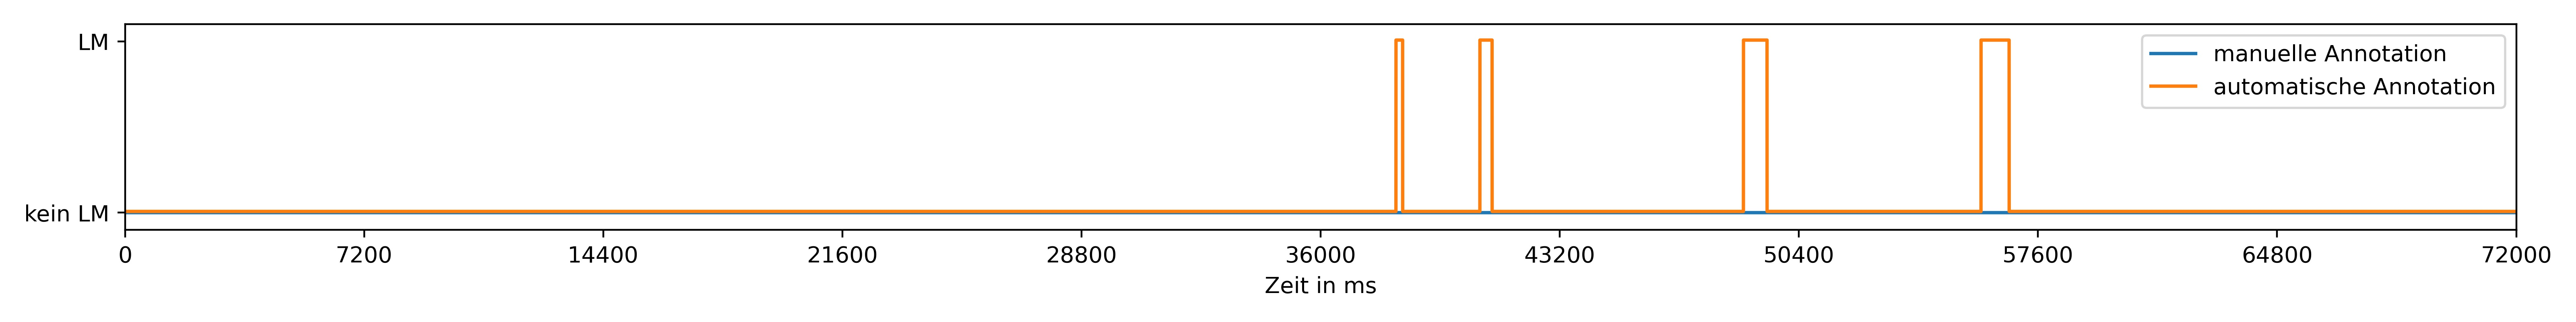
\includegraphics[width=0.80\textwidth]{./Bilder/vorrübergehendesRauschenacq_002963603.edf108000,72000.jpg}
	\end{center}
	\caption{Ausschnitt eines unregelmäßigen EMG-Signals zur Veranschaulichung der dynamischen Anpassung des Schwellwertes (oben) und die daraus resultierende automatischer Annotation (unten). Die Abtastfrequenz beträgt 200 Hz.}%
	\label{fig:detectorWorking}%
\end{figure}


Das folgende Signal (Abb. \ref{fig:EKG}) zeigt einen Ausschnitt einer EKG Störung mit einer Herzfrequenz von ungefähr einem Hertz und den daraus resultierenden erhöhten oberen Schwellwert. Durch diese Einkopplungen sind Beinbewegungen nicht mehr klar erkennbar.

\begin{figure}[!ht]%
	\begin{center}
	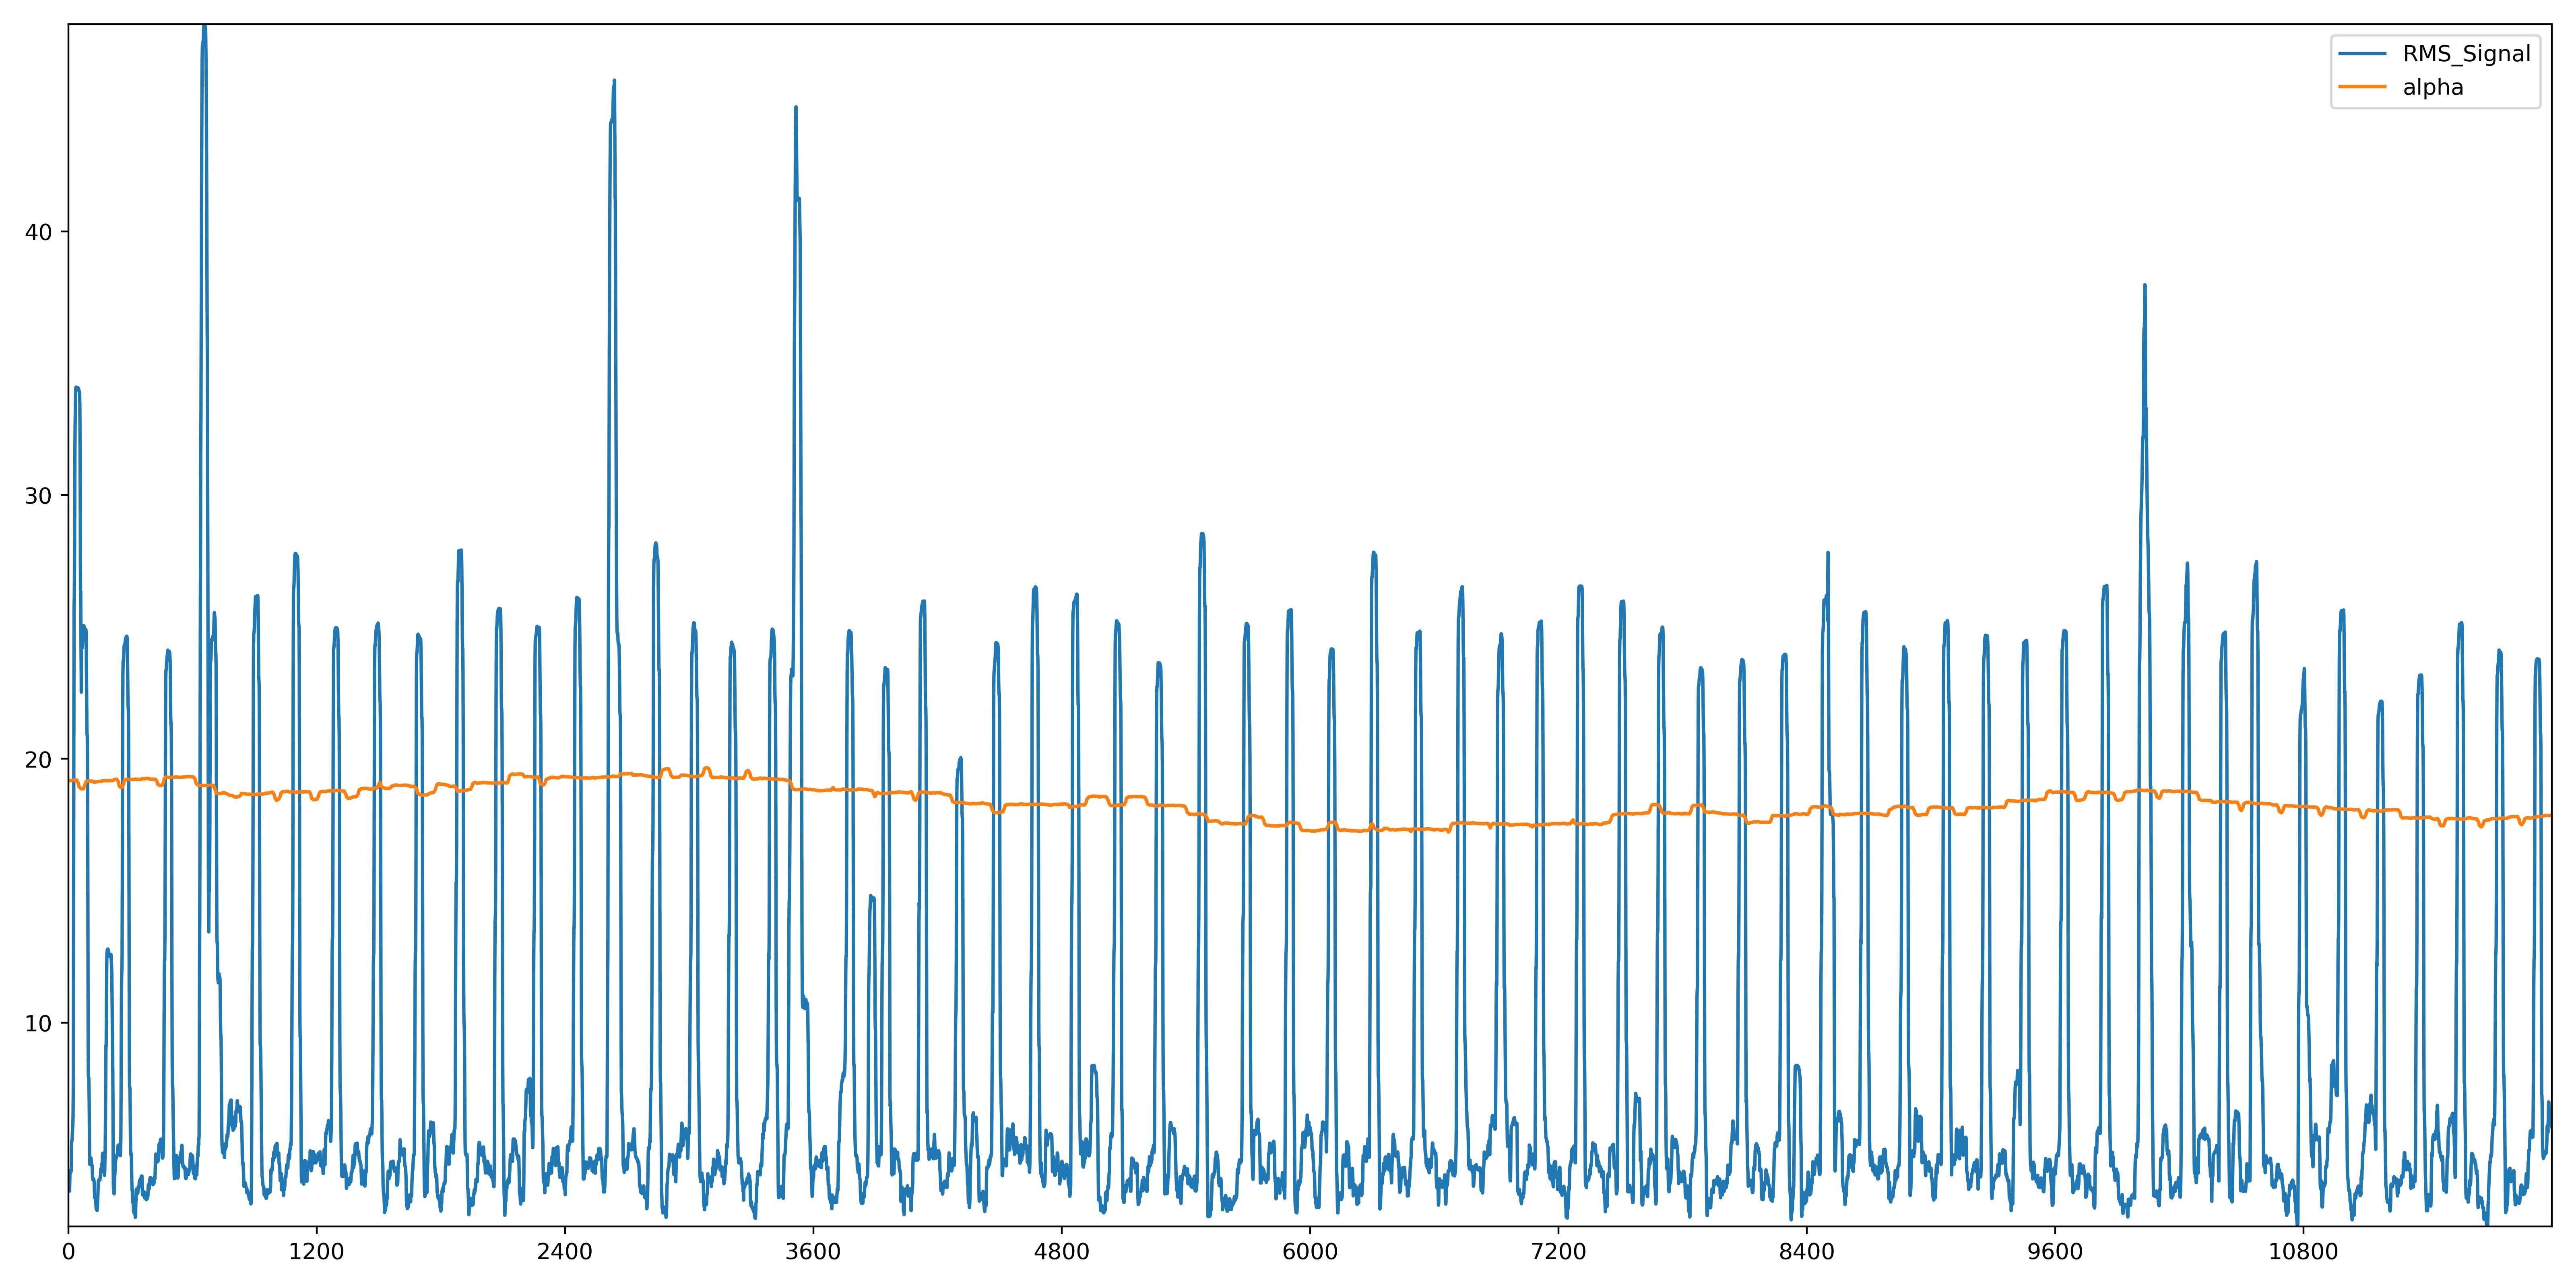
\includegraphics[width=0.80\textwidth]{./Bilder/maybeNoiseNoIdeaWhatHappenedEMGacq_002963603.edf276000,12000.jpg}
	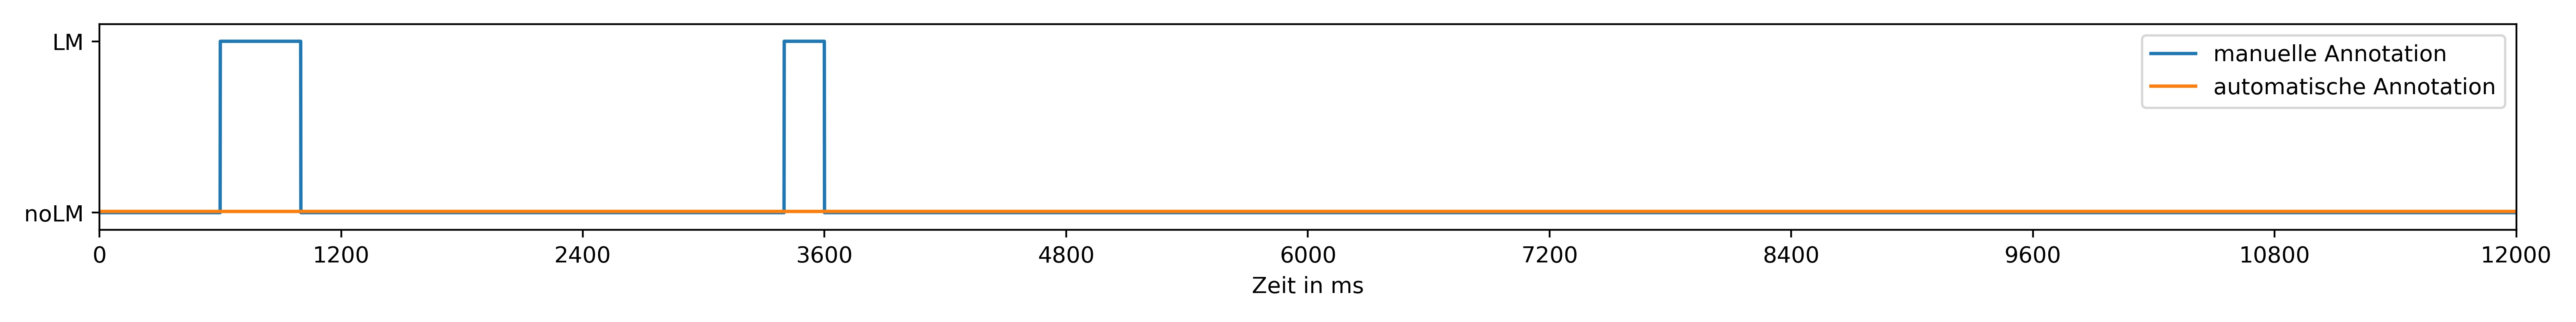
\includegraphics[width=0.80\textwidth]{./Bilder/maybeNoiseNoIdeaWhatHappenedacq_002963603.edf276000,12000.jpg}
	\end{center}
	\caption{EMG-Signal mit EKG Einkopplung (oben), bei der die manuell annotierten Beinbewegungen von dem Detektor nicht erkannt wurden.}%
	\label{fig:EKG}%
\end{figure}

 \newpage
\chapter{Ergebnisse}

\section{Klassische Metriken}

In den Tabellen \ref{tab:eventweise 1} und \ref{tab:eventweise 2} wird der in dieser Arbeit implementierte Detektor mit den Detektoren aus der Literatur anhand eventweise berechneter klassischen Metriken verglichen. Zu beachten ist, dass der Detektor größtenteils aus der Veröffentlichung von Moore et al. \cite{Moore} übernommen wurde.
In der Statistik wurden Annotationen ausgeschlossen, bei denen die jeweilige Metrik unendlich wurde.
Die Mittelwerte werden stark durch die große Abweichung weniger Extremfälle beeinflusst. Um die Verteilung besser zu repräsentieren wurde zusätzlich der Median angegeben.


\begin{table}[!ht]
    \caption{Stand der Technik für eventweise Auswertung zur Einordnung des implementierten Detektors, Teil 1; Der Zusatz 'r' bezeichnet einen rekonstruierten Wert}   
	\centering
		\begin{tabular}{llllllllll}
			\hline & \cite{Huang} & \cite{Moore} & \cite{Moore} & \cite{alvarez} & \cite{ferri}\\
			\hline {$\!\begin{aligned}
				&\\
			    Datensatz\\
			    Art\ des\ Klassifikators\\
			    Berechnungsart\\
			    \gls{Sens}\\
			    \gls{Prec}\\
			    \gls{Spez}\\
			    \gls{NPV}\\
			    \gls{Acc}\\
			    Cohens\ \kappa\\
			    F1-Ma"s\\
			    Korrealtion\ PLM/h\\
			    relative\ \#\ PLM\\
				&\\
				\end{aligned}$} & {$\!\begin{aligned}
				&\\
				15\ \gls{RLS}\ (24)\\
				statisch\\
				Event\\
				0.95\\
				-\\
				0.92\\
				-\\
				-\\
				-\\
				0.93r\\
				0.97\\
				1\\
				&\\
				\end{aligned}$} & {$\!\begin{aligned}
				&\\
				\acrshort{WSC}\ (1073)\\
				dynamisch\\
			    Event\ \cite{git}\\
				0.6\\
				0.88\\
				1\\
				0.99\\
				0.98\\
				0.71\\
				-\\
				0.94\\
				0.63\\
				&\\
				\end{aligned}$} & {$\!\begin{aligned}
				&\\
				\acrshort{SSC}\ (760)\\
				dynamisch\\
				Event\ \cite{git}\\
				0.75\\
				0.82\\
				1\\
				0.99\\
				0.99\\
				0.87\\
				-\\
				0.94\\
				0.92\\
				&\\
				\end{aligned}$}  & {$\!\begin{aligned}
				&\\
			    \acrshort{HMC}\ (70)\\
				dynamisch\\
				Segment\ (1s)\\
				0.82\\
				0.71\\
				1\\
				-\\
				1\\
				0.73\\
				0.73\\
				-\\
				0.99\\
				&\\
				\end{aligned}$}  & {$\!\begin{aligned}
				&\\
				\acrshort{WSC}\ (60)\\
				statisch.\\
				Event\\
				0.85\\
				0.62\\
				0.99\\
				1\\
				0.99\\
				0.72\\
				-\\
				-\\
				1.3\\
				&\\
				\end{aligned}$}
				\\
				\hline
		\end{tabular}

\label{tab:eventweise 1}
\end{table}


\begin{table}[!ht]
    \caption{Stand der Technik für eventweise Auswertung zur Einordnung des implementierten Detektors, Teil 2}   
	\centering
		\begin{tabular}{lllllllllll}
			\hline & \cite{wetter} & \cite{Carvelli}& \cite{Carvelli}& \cite{Carvelli}& implement. Detektor\\
			\hline {$\!\begin{aligned}
			    &\\
			    Datensatz\\
			    Klassifikatorart\\
			    Berechnungsart\\
			    \gls{Sens}\\
			    \gls{Prec}\\
			    \gls{Spez}\\
			    \gls{NPV}\\
			    \gls{Acc}\\
			    Cohens\ \kappa\\
			    F1-Ma"s\\
			    Korrealtion\ PLM/h\\
			    relative\ \#\ PLM\\
				&\\
				\end{aligned}$} & {$\!\begin{aligned}
				&\\
				\acrshort{WSC}\ (60)\\
				statisch\\
				Event\\
				0.96\\
				0.47\\
				0.98\\
				1\\
				0.98\\
				0.62\\
				-\\
				-\\
				2\\
				&\\
				\end{aligned}$} & {$\!\begin{aligned}
				&\\
                \acrshort{WSC}\ (275)\\
				\acrshort{DNN}\\
				Event\\
				0.9\\
				0.81\\
				-\\
				-\\
				-\\
				-\\
				0.83\\
				-\\
				-\\
				&\\
				\end{aligned}$}& {$\!\begin{aligned}
				&\\
                \acrshort{SSC}\ (177)\\
				\acrshort{DNN}\\
				Event\\
				-\\
				-\\
				-\\
				-\\
				-\\
				-\\
				0.71\\
				-\\
				-\\
				&\\
				\end{aligned}$}& {$\!\begin{aligned}
				&\\
                \acrshort{MrOS}\ (348)\\
				\acrshort{DNN}\\
				Event\\
				-\\
				-\\
				-\\
				-\\
				-\\
				-\\
				0.77\\
				-\\
				-\\
				&\\
				\end{aligned}$} & {$\!\begin{aligned}
				&\\
                Uniklinik\ DD\ (5908)\\
                dynamisch\\
				Event\\
				0.6\\
				0.68\\
				0.84\\
				0.78\\
				0.72\\
				0.41\\
				0.57\\
    			0.48\\
    			1.4\\
				&\\
				\end{aligned}$}
				\\
				\hline
		\end{tabular}

\label{tab:eventweise 2}
\end{table}

In Tabelle \ref{tab:segemtnweise} ist gesondert der Vergleich der segmentweisen Auswertung zu sehen. Zu beachten ist, dass in dem implementierten Detektor besonders die Metriken einen hohen Wert aufweisen, die ein \gls{TN} im Zähler haben.
\begin{table}[!ht]
    \caption{Stand der Technik für segmentweise Auswertung zur Einordnung des implementierten Detektors}   
	\centering
		\begin{tabular}{lll}
			\hline & \cite{alvarez} & implement. Detektor\\
			\hline {$\!\begin{aligned}
			    &\\
			    Datensatz\\
			    Klassifikatorart\\
			    Berechnungsart\\
			    \gls{Sens}\\
			    \gls{Prec}\\
			    \gls{Spez}\\
			    \gls{NPV}\\
			    \gls{Acc}\\
			    Cohens\ \kappa\\
			    F1-Ma"s\\
			    Korrealtion\ PLM/h\\
			    relative\ \#\ PLM\\
				&\\
				\end{aligned}$} & {$\!\begin{aligned}
				&\\
				\acrshort{HMC}\ (70)\\
				dyn.\\
				Segment\ (1s)\\
				0.82\\
				0.71\\
				1\\
				-\\
				1\\
				0.73\\
				0.73\\
				-\\
				0.99\\
				&\\
				\end{aligned}$} & {$\!\begin{aligned}
				&\\
                Uniklinik\ DD\ (5908)\\
                dyn.\\
				Segment\ (1s)\\
				0.49\\
			    0.6\\
				0.99\\
			    0.98\\
				0.97\\
				0.46\\
				0.47\\
    			0.48\\
    			1.4\\
				&\\
				\end{aligned}$}
				\\
				\hline
		\end{tabular}

\label{tab:segemtnweise}
\end{table}


\section{Kostenfunktional}
\begin{table}[!ht]
    \caption{Korrelation zwischen Kostenfunktional und klassischen Metriken}
	\centering
		\begin{tabular}{llllllll}
			\hline & F1-Ma"s& Cohens $\kappa$ & \gls{Spez} & \gls{Prec} & \gls{Sens}& \gls{Acc}& \gls{NPV}\\
			\hline {$\!\begin{aligned}
				&\\
				Kostenfunktional\\
				&\\
				\end{aligned}$} & {$\!\begin{aligned}
				&\\
			    -0.184\\
				&\\
				\end{aligned}$}& {$\!\begin{aligned}
				&\\
			    -0.125\\
				&\\
				\end{aligned}$}& {$\!\begin{aligned}
				&\\
			    0.251\\
				&\\
				\end{aligned}$}& {$\!\begin{aligned}
				&\\
			    0.175\\
				&\\
				\end{aligned}$}& {$\!\begin{aligned}
				&\\
			    -0.262\\
				&\\
				\end{aligned}$}& {$\!\begin{aligned}
				&\\
			    -0.159\\
				&\\
				\end{aligned}$}& {$\!\begin{aligned}
				&\\
			    -0.283\\
				&\\
				\end{aligned}$}\\
			    \hline
		\end{tabular}

\label{tab:KorrMetriken}
\end{table}


Das Kostenfunktional korreliert nur schwach mit den klassischen Metriken (siehe Tabelle \ref{tab:KorrMetriken}).

Die Tabelle \ref{tab:Kostenbeiträge} schlüsselt die Beiträge der verschiedenen Fehler zu der Gesamtkostenzahl auf.
Zur besseren Einordnung der Mittelwerte sind zusätzlich noch die Anzahl der Annotationen aufgelistet, die keine Kosten verursacht haben. Die relativen Kosten sind definiert durch die absoluten Kosten bezogen auf die manuelle PLM Anzahl.
An dieser Aufschlüsselung der Kosten ist interessant, dass wenig Fehler durch Xto1- und 1toX- Matches entstanden sind.
Die Hauptfehlerquelle ist eine Verminderung der PLM Anzahl aufgrund von \gls{FN} (41 Prozent).

\begin{table}[!ht]
\caption{Beiträge der Fehlerarten an den Gesamtkosten. (+) hinter der Fehlerart beschreibt, dass dieser Fehler zu einer Erhöhung des PLM-Indexes geführt hat. (-) steht analog für eine Verminderung.}
	\centering
		\begin{tabular}{lll}
			\hline Fehlerart & Mittelwert & \# Dateien ohne Kosten\\
			\hline {$\!\begin{aligned}
				&\\
				FP\ (+)\\
				1toX\ (+)\\
				Zeitungenauigkeiten\ (+)\\
				FN\ (-)\\
    			Xto1\ (-)\\
				Zeitungenauigkeiten\ (-)\\
				absolute\ Kosten\\
				relative\ Kosten\\
			
				&\\
				\end{aligned}$} & {$\!\begin{aligned}
				&\\
				42\\
				1.25\\
				72\\
				117\\
				2.05\\
				72.9\\
				285\\
				2.26\\
				&\\
				\end{aligned}$} & {$\!\begin{aligned}
				&\\
				1341\\
				4718\\
				1108\\
				873\\
				4274\\
				988\\
				488\\
				488\\
				&\\
				\end{aligned}$}\\
				\hline
		\end{tabular}

\label{tab:Kostenbeiträge}
\end{table}


Die Differenz aus ergebniserhöhenden Fehlern und ergebnisvermindernden Fehlern ($K_{diff}$) korreliert gut mit der Differenz aus automatisch annotierten PLM und manuell annotierten PLM (siehe Bild \ref{fig:plotKorr}). Der Korrelationskoeffizient liegt bei 0.987. Dieser Wert beschreibt den Zusammenhang zwischen den erklärten Fehlern aus dem Kostenfunktional und dem medizinisch wichtigen PLM-Index.


Die Verteilugen der absoluten und relative Kosten (absolute Kosten bezogen auf die manuelle PLM-Anzahl) sind in Abb. \ref{fig:Kostennebeneinander} dargestellt. Es ist zu erkennen, dass Annotationen an denen höhere Kosten entstanden sind, seltener sind. 

\begin{figure}[!ht]%
	\begin{center}
	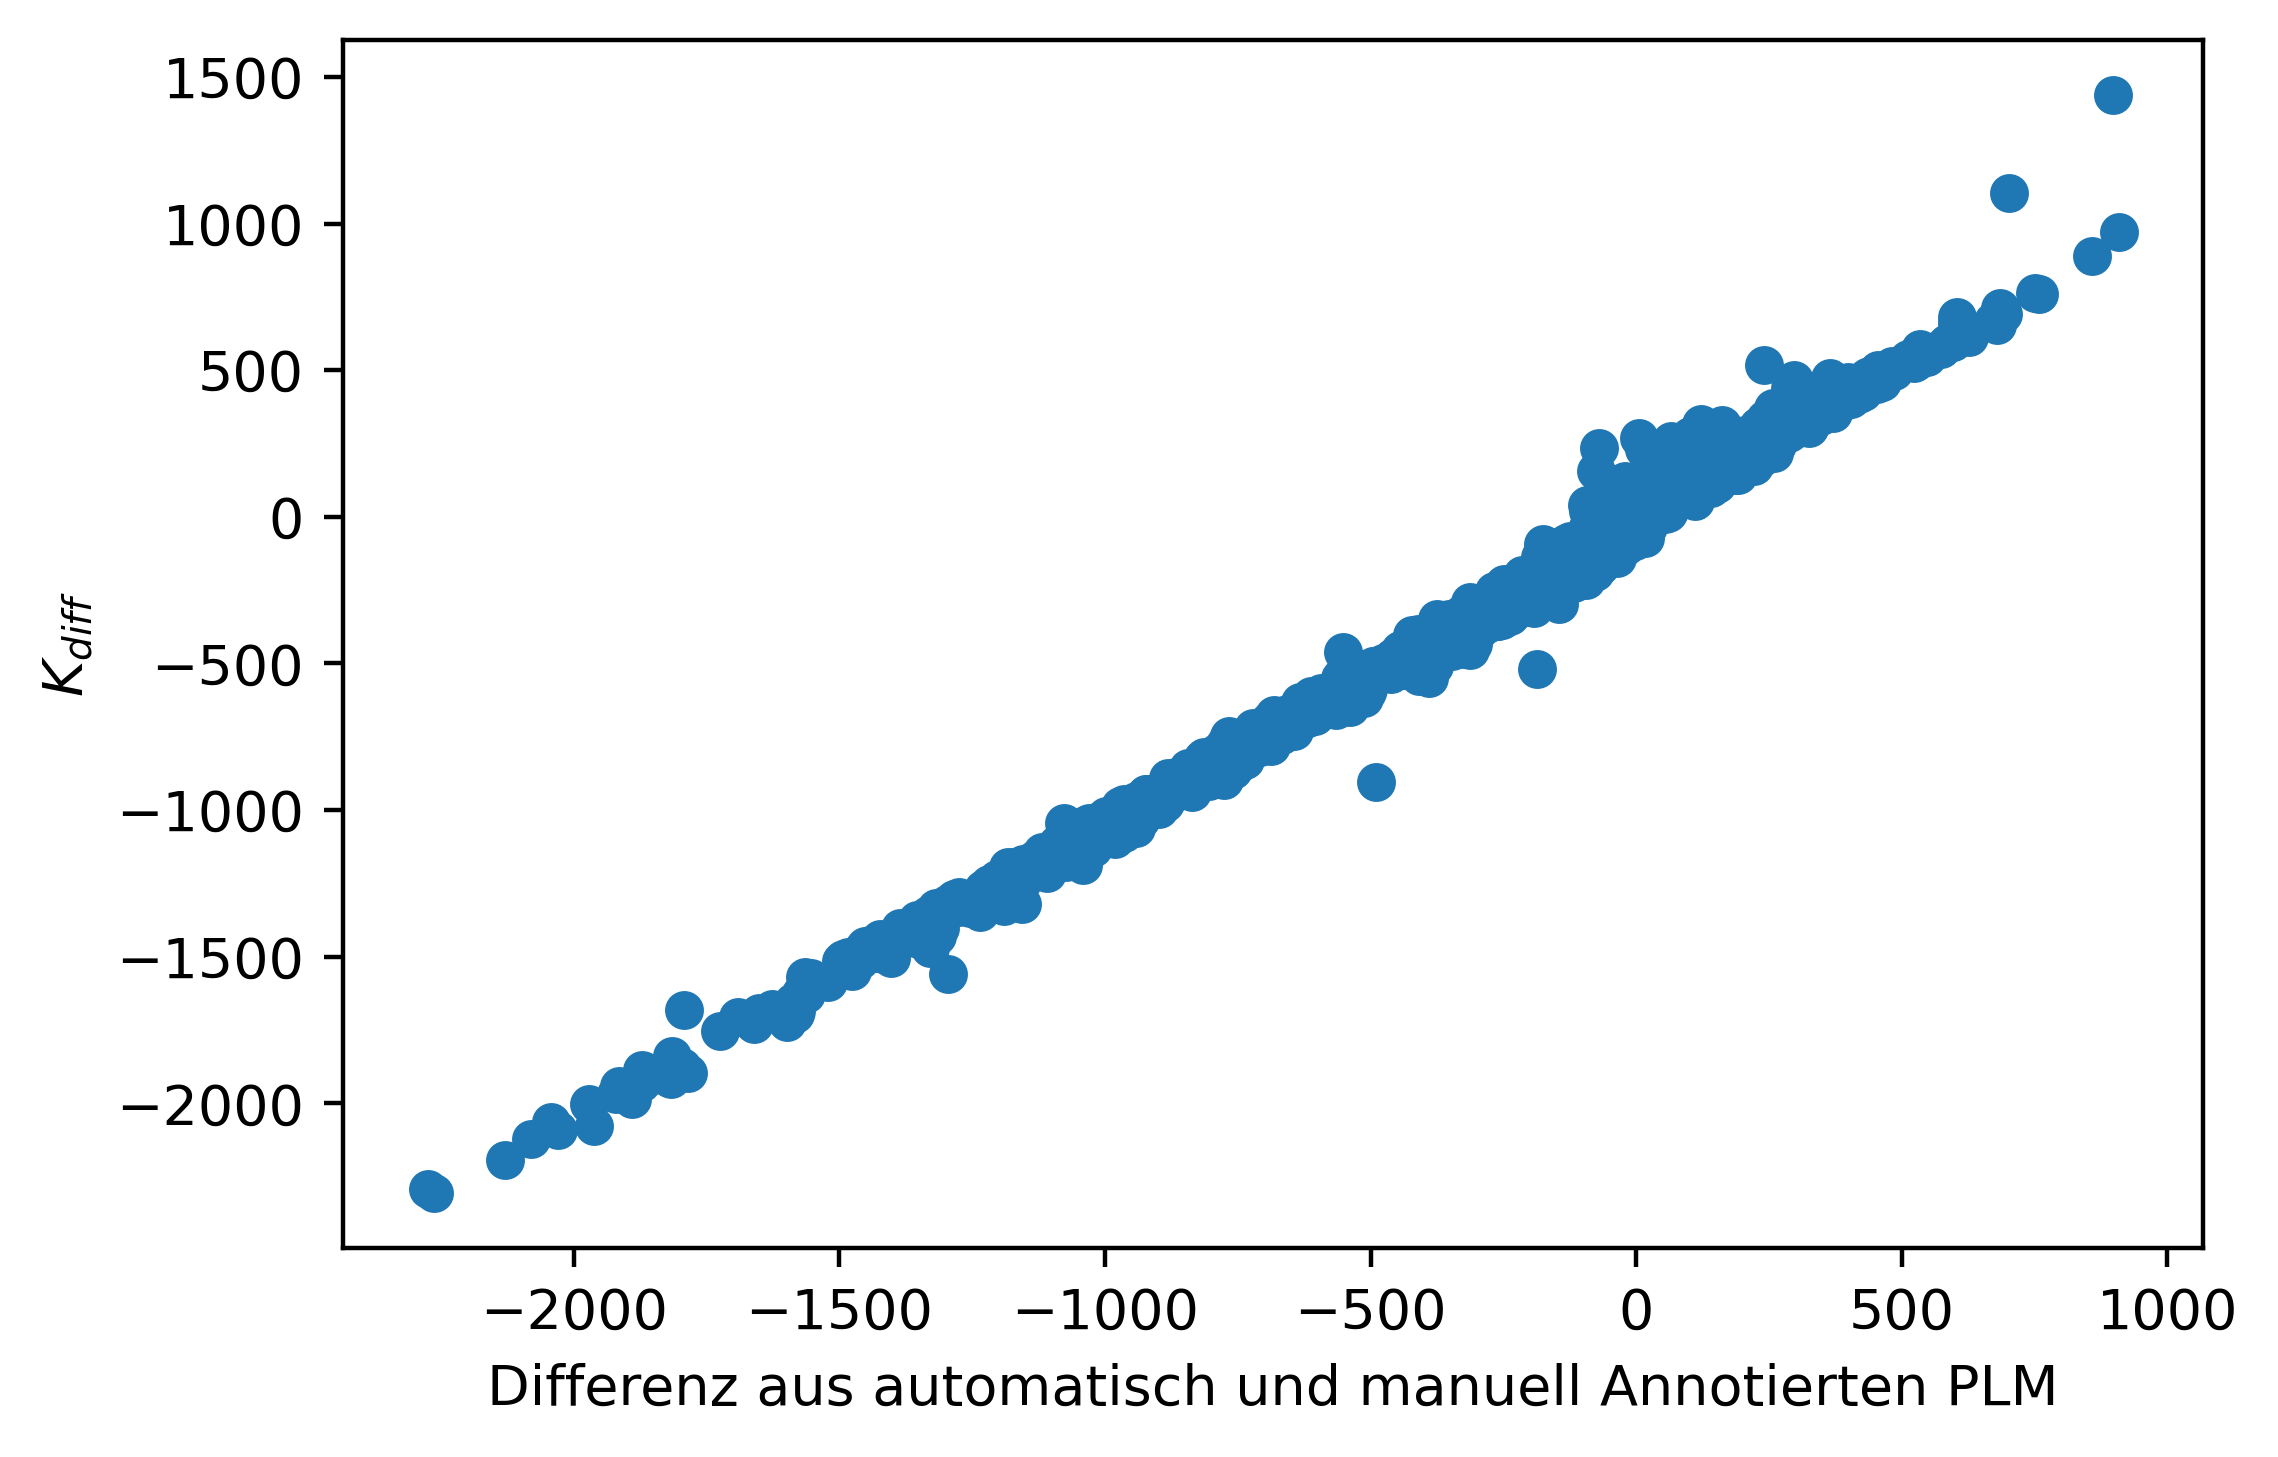
\includegraphics[width=0.80\textwidth]{./Bilder/korre.png}
	\end{center}
	\caption{Veranschaulichung der Korrelation von Differenz aus ergebniserhöhenden Fehlern und ergebnisvermindernden Fehlern ($K_{diff}$) und Differenz aus automatisch annotierten und manuell annotierten PLM.}%
	\label{fig:plotKorr}%
\end{figure}

\begin{figure}[!ht]%
\centering
	\begin{subfigure}[t]{.49\linewidth}%
		\centering
		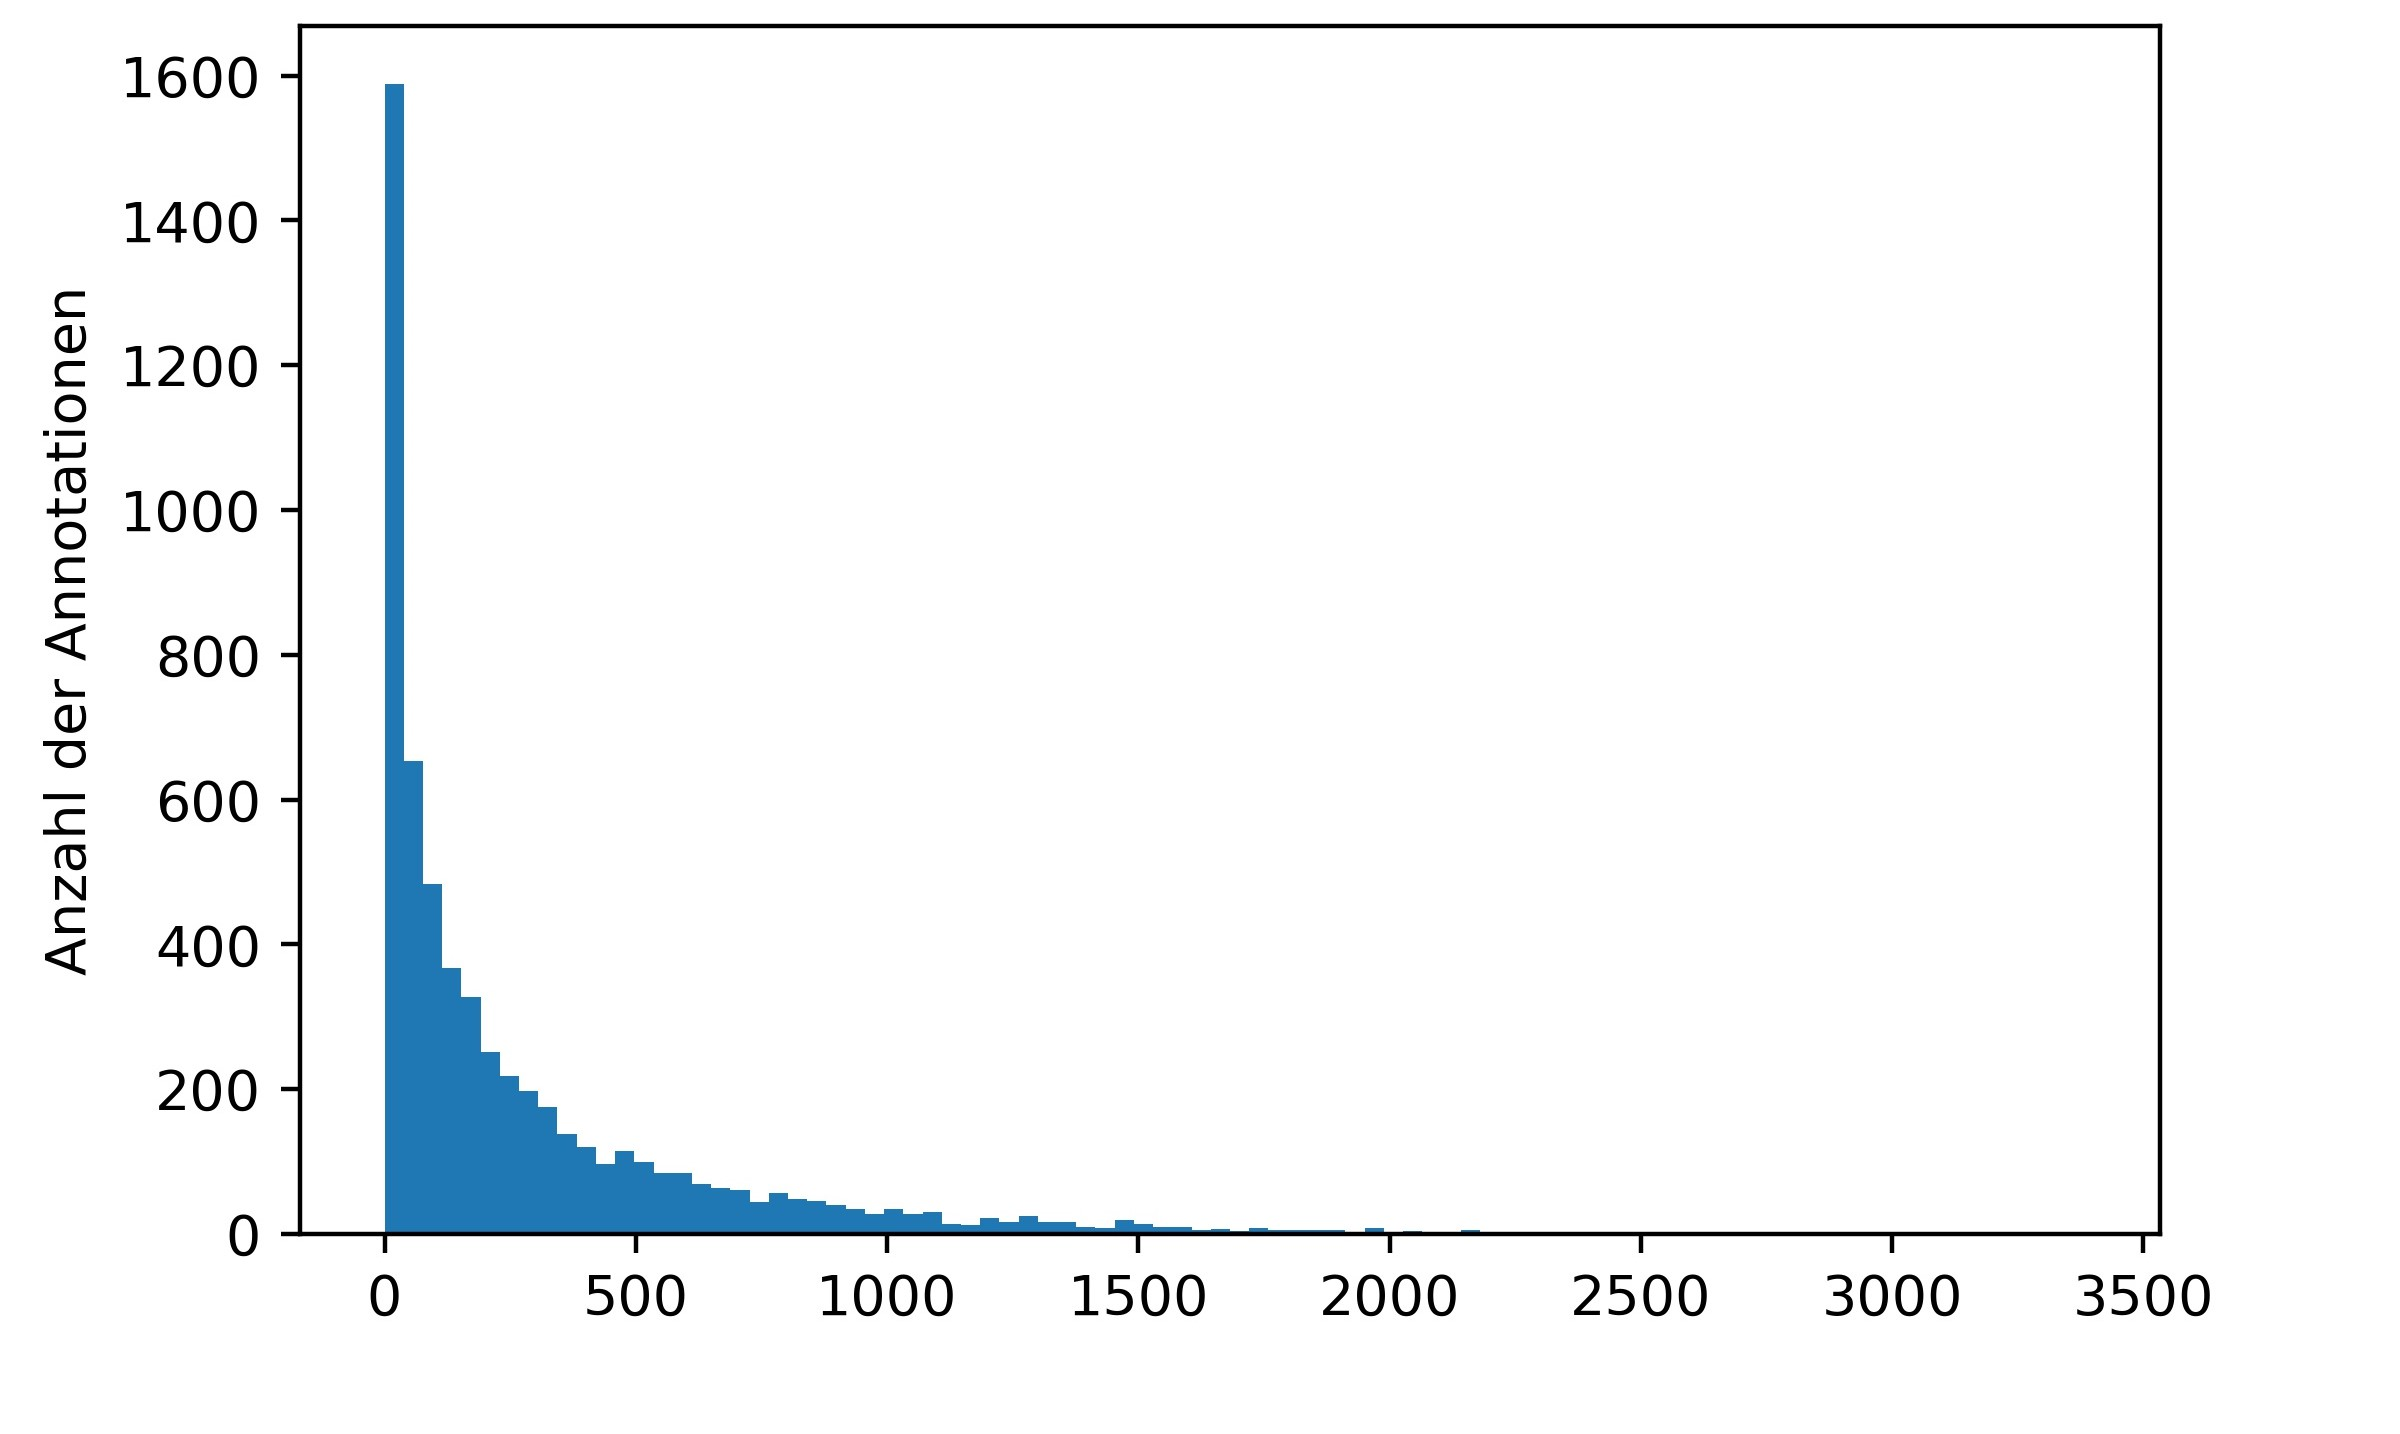
\includegraphics[width=0.80\textwidth]{./Bilder/absolute Kosten.jpg}
		\caption{Histogrammm der absoluten Kosten}
	\end{subfigure}
	\begin{subfigure}[t]{.49\linewidth}%
		\centering
		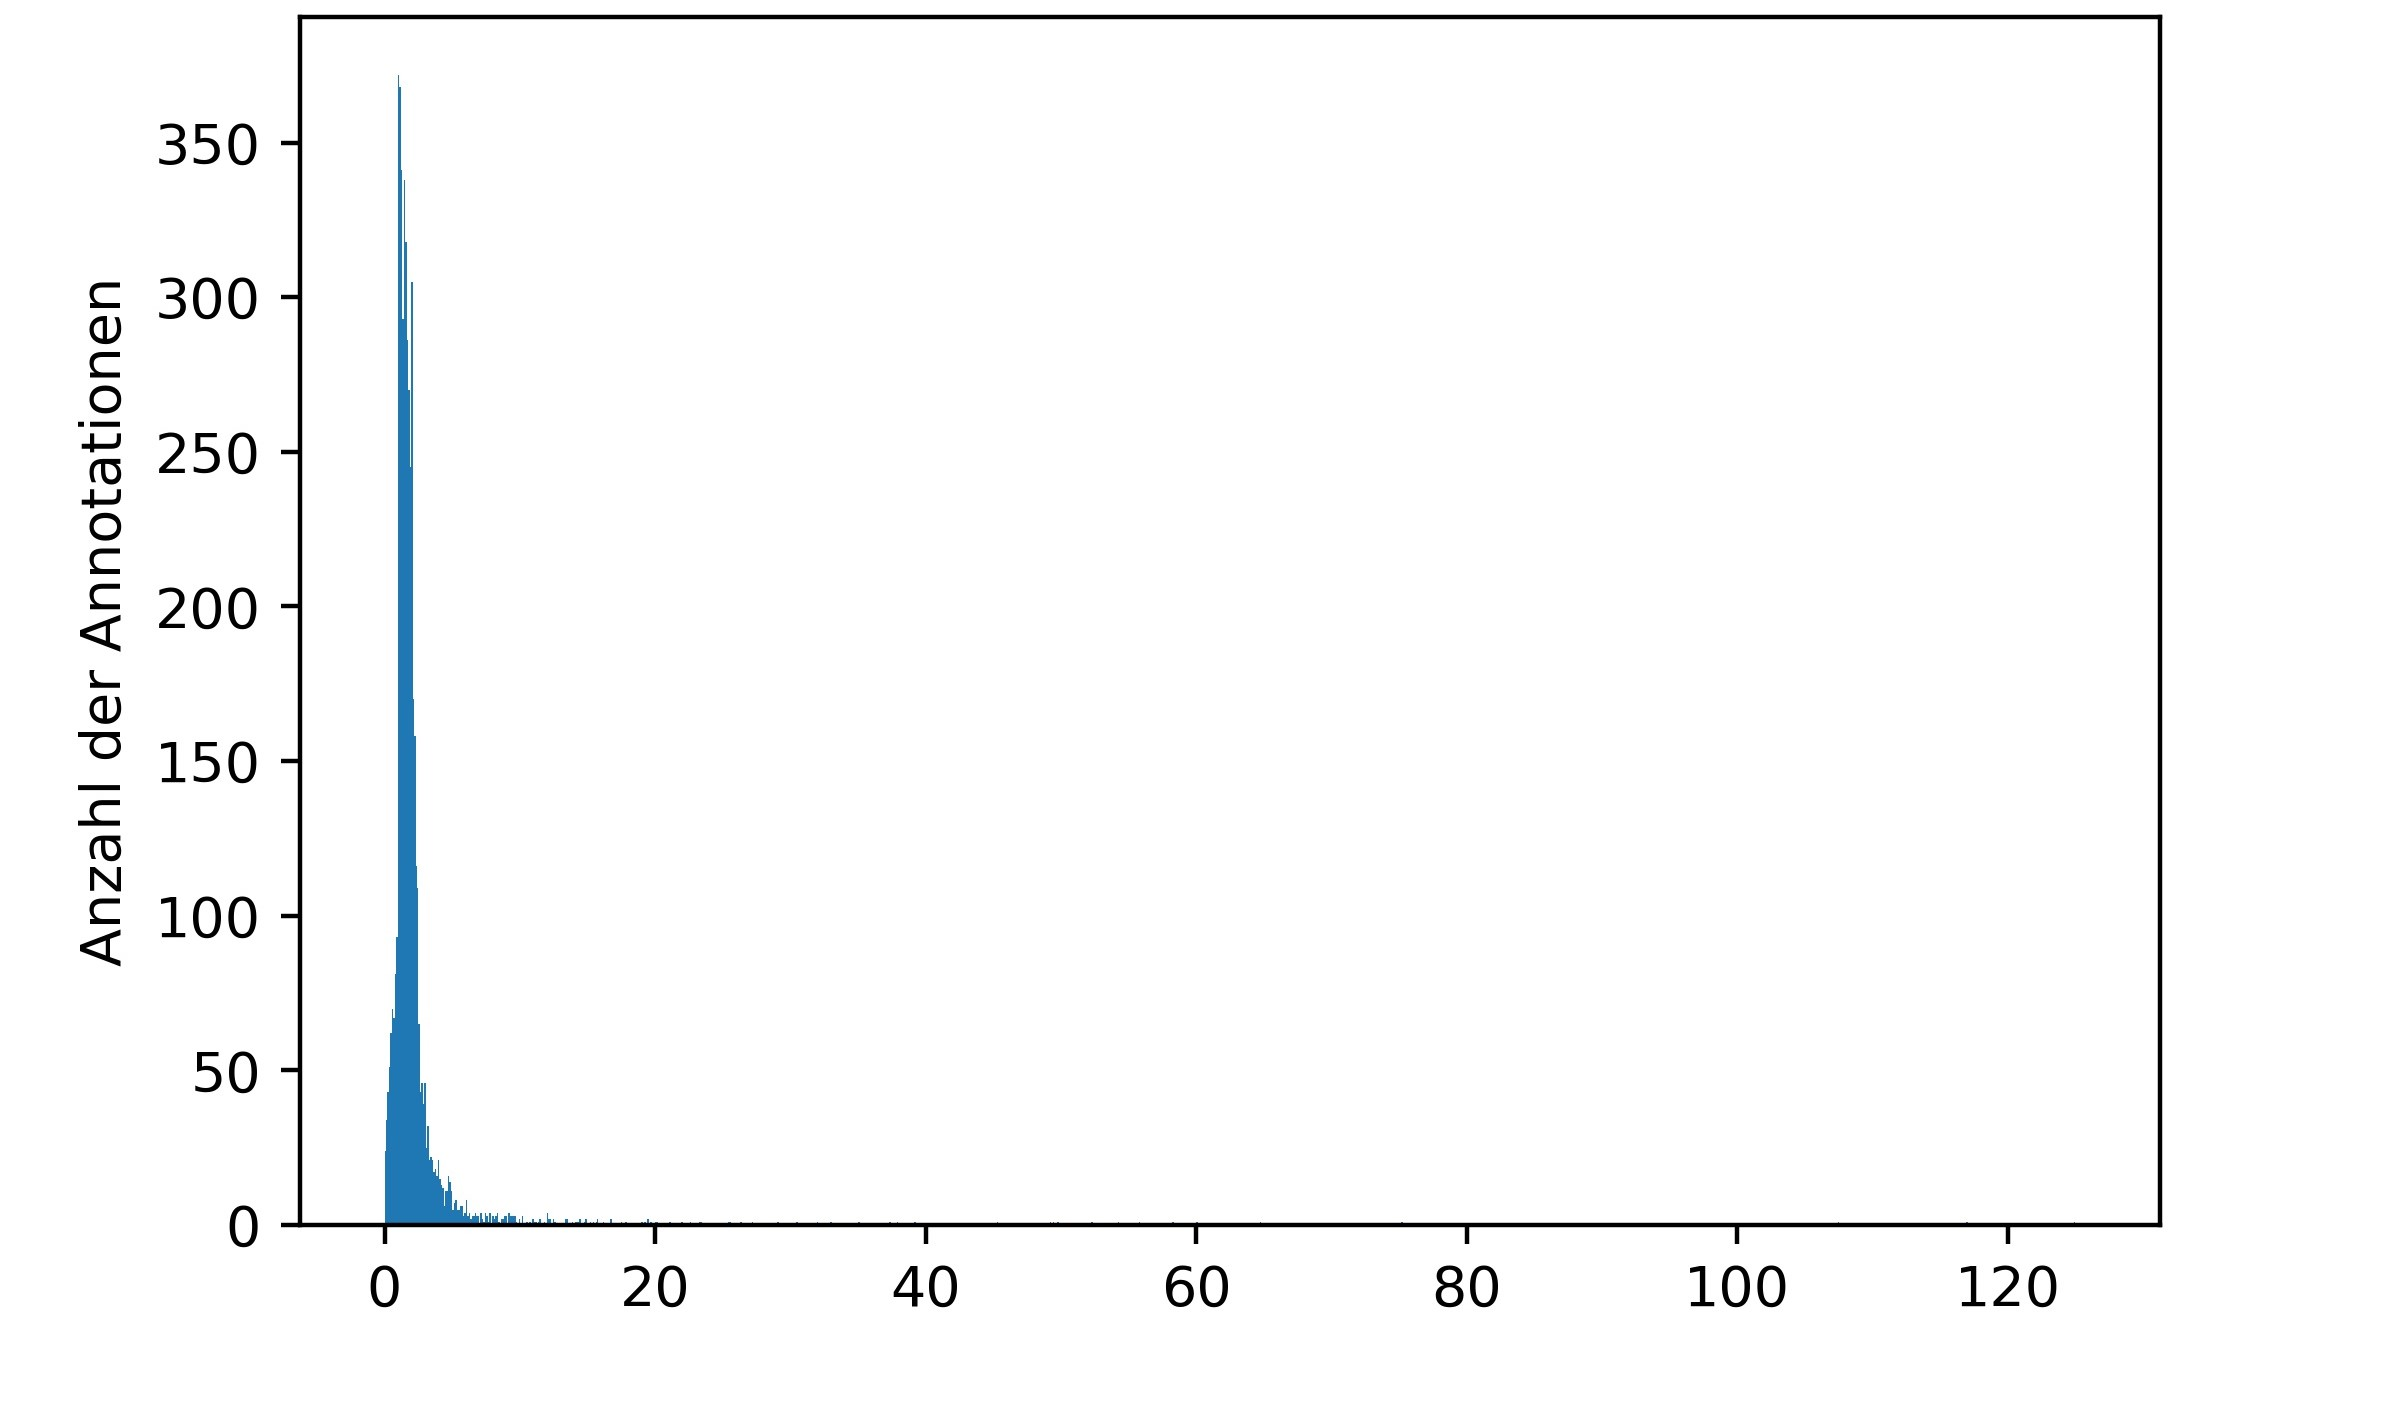
\includegraphics[width=0.8\textwidth]{./Bilder/relative Kosten.jpg}
		\caption{Histogrammm der relativen Kosten}
	\end{subfigure}
\caption{Darstellung der Kostenverteilung mit einer automatisch erstellten Balkenweite}
\label{fig:Kostennebeneinander}
\end{figure}



\section{Verbesserung der Einordnung des Detektors}
Die Metriken zu Verbesserung der Einordnung des Detektors sind in Tabelle \ref{tab:VerbesserungMetriken} zu sehen. Der Anhang "mean" beschreibt den Mittelwert der Verteilung über die Differenz der Start- oder Endzeitpunkte von TP. Die Anhand "std" beschreibt analog die Standardabweichung der Verteilung.
\begin{table}[!ht]
\caption{Metriken aus dem Kapitel \ref{Verbesserung}: "Verbesserung der Einordnung des Detektors"}
	\centering
		\begin{tabular}{lll}
			\hline & Mittelwert & Median\\
			\hline {$\!\begin{aligned}
				&\\
				Falsch\ positiv\ Rate\\
    			Verstö"se\ gegen\ die\ LM-Zeitkriterien\\
				Anzahl\ der\ Xto1-Matches\\
				Anzahl\ der\ 1toX-Matches\\
    			Schwerpunkt\\
		        LM-Anzahl\ (automatisch\ / \ manuell)\\
				Startzeitpunkte_{mean}\\
				Startzeitpunkte_{std}\\
				Endzeitpunkte_{mean}\\
				Endzeitpunkte_{std}\\
			
				&\\
				\end{aligned}$} & {$\!\begin{aligned}
				&\\
				0.55\\
				0\\
				2.9\\
				1.6\\
				136\ Sekunden\\
				1.6\\
				-0.38\ Sekunden\\
				0.83\ Sekunden\\
				0.76\ Sekunden\\
				1.2\ Sekunden\\
				&\\
				\end{aligned}$} & {$\!\begin{aligned}
				&\\
				0.56\\
				0\\
				0\\
				0\\
			    50\ Sekunden\\
				0.89\\
				-0.26\ Sekunden\\
				0.67\ Sekunden\\
				0.64\ Sekunden\\
				1\ Sekunde\\
				&\\
				\end{aligned}$}\\
				\hline
		\end{tabular}

\label{tab:VerbesserungMetriken}
\end{table}

Zur besseren Einordnung der LM Verhältnisse wurde die Differenz der Anzahl zwischen automatisch und manuell annotierten LM berechnet. Der Mittelwert beträgt -87.1. Da das Vorzeichen negativ ist, wurden im Mittel mehr manuelle LM annotiert.


Das Histogramm über alle Schwerpunktdifferenzen ist in Grafik \ref{fig:centers} dargestellt. Es sind keine Teilmengen im Histogramm zu erkennen, die die Festsetzung eines Schwellwertes erlauben würden.
\begin{figure}[!ht]%
	\begin{center}
	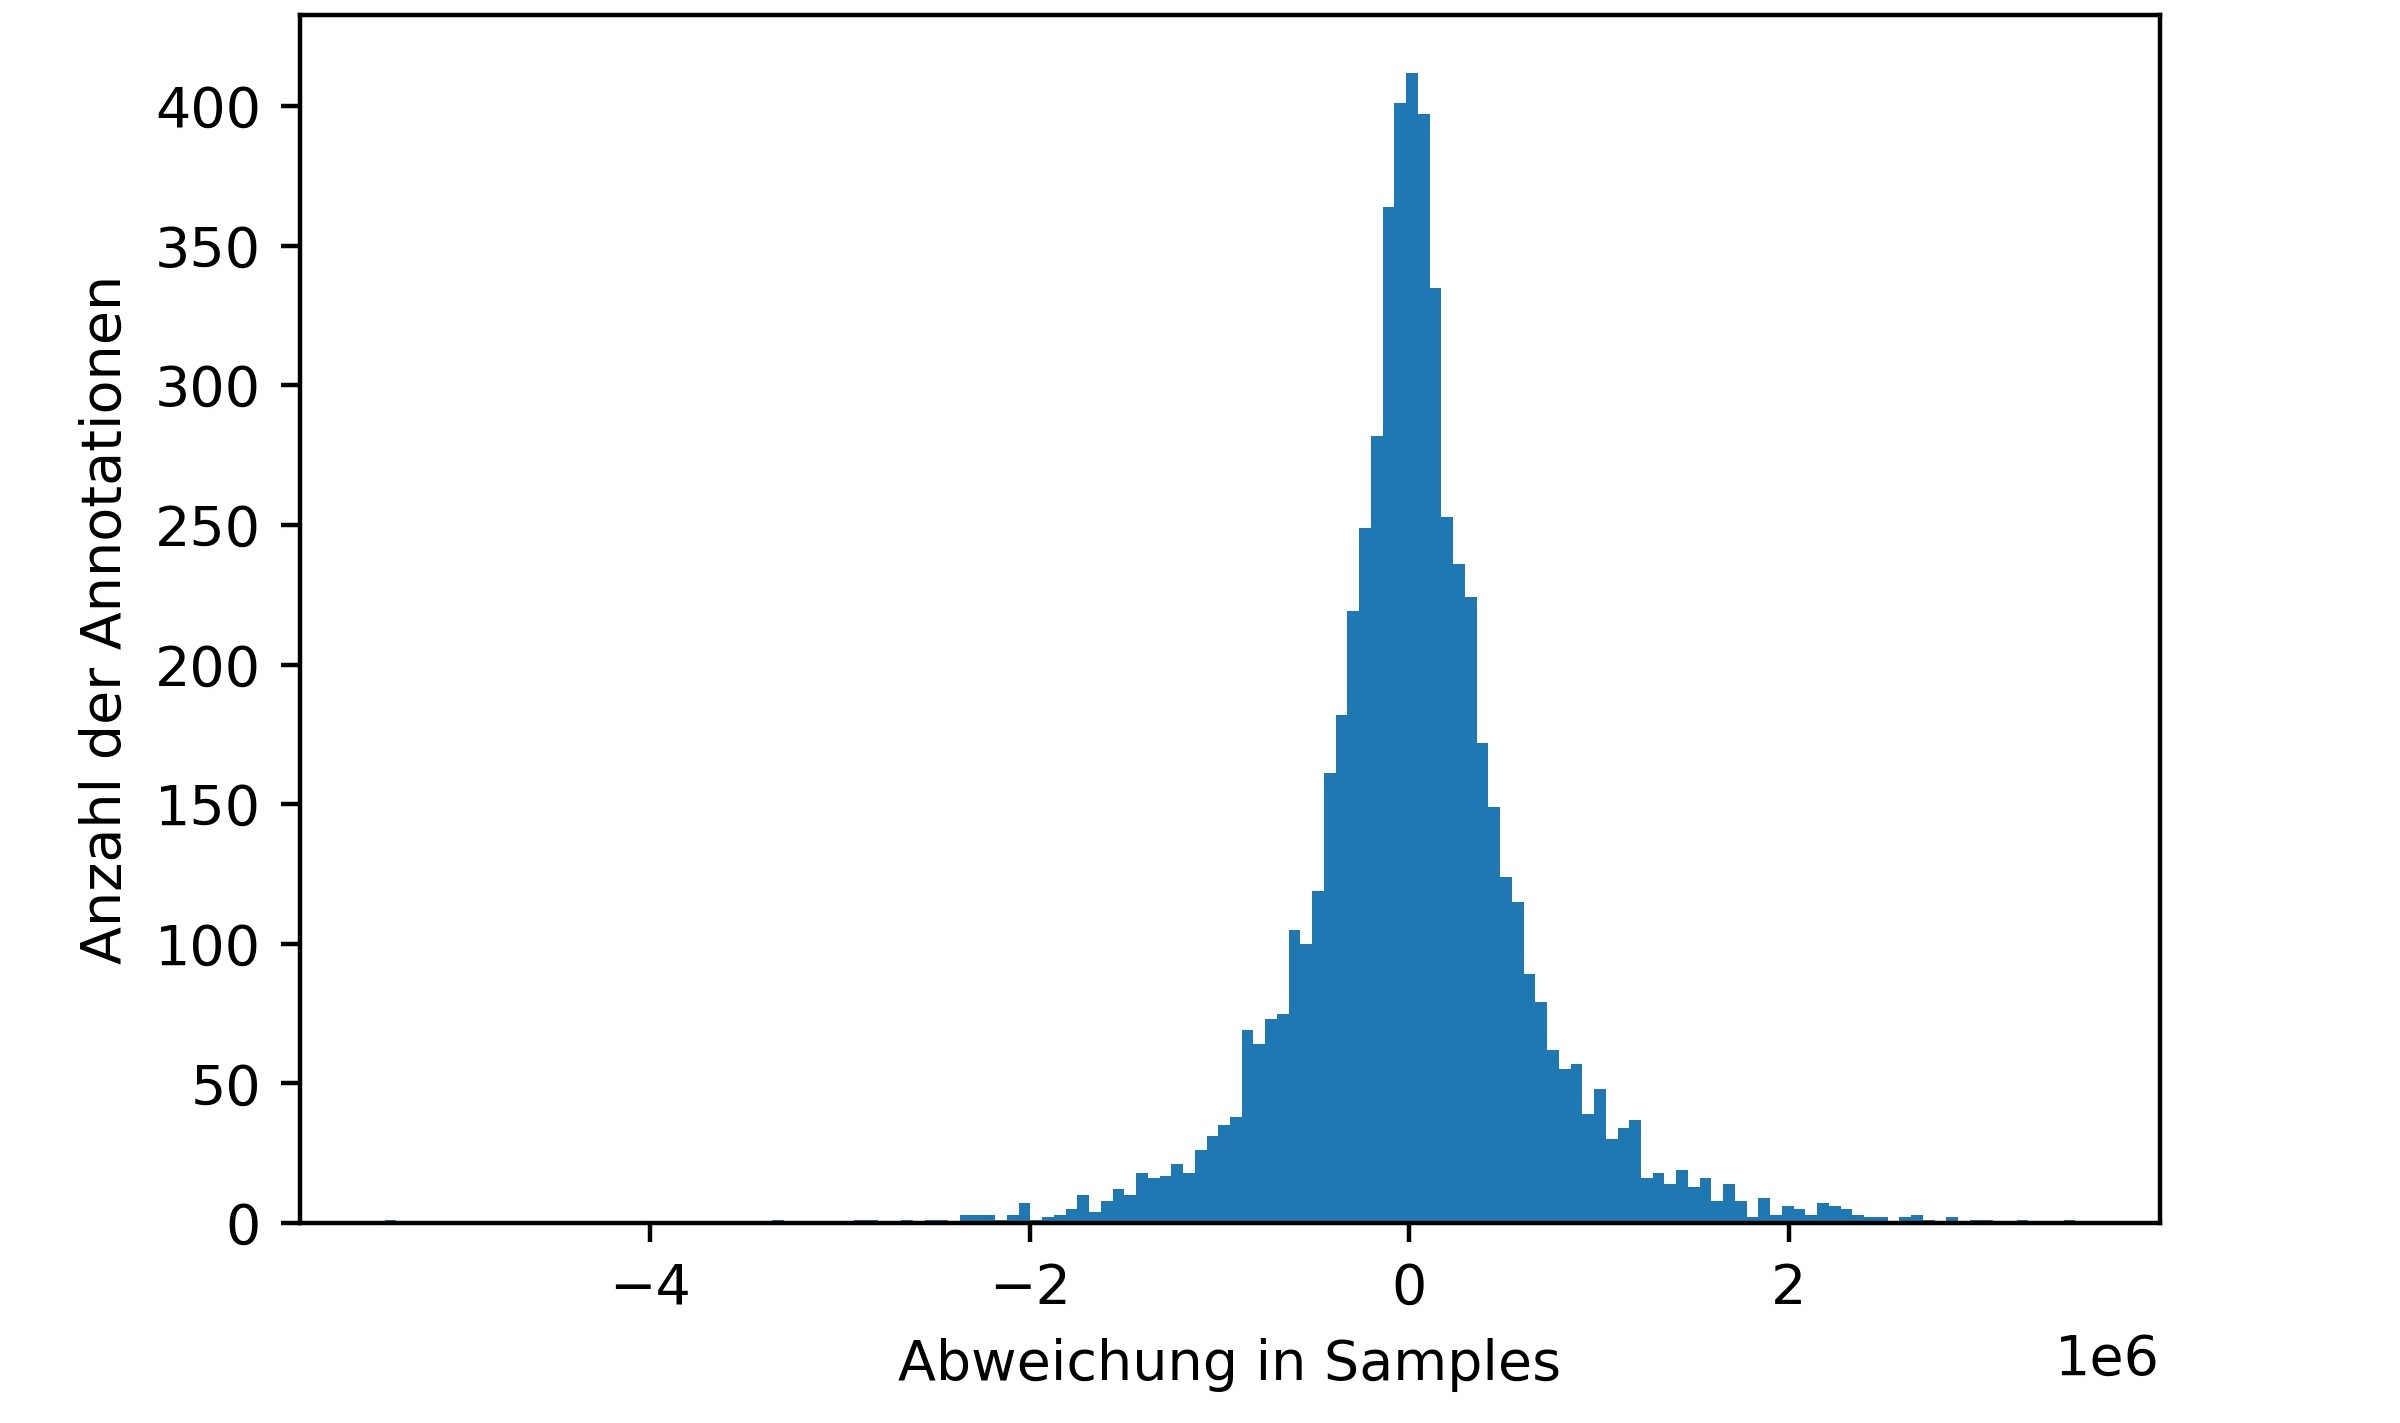
\includegraphics[width=0.80\textwidth]{./Bilder/centers.jpg}
	\end{center}
	\caption{Histogramm über die Differenz der Schwerpunkte aus automatischer und manueller Annotation. Die Breite der Balken wurde für die gesamte Arbeit automatisch erstellt.}%
	\label{fig:centers}%
\end{figure}

Dieses Histogramm zeigt die falsch positiv Rate. Die Häufung um den Wert 0.5 deutet darauf hin, dass FP und TN ähnlich häufig vorkommen. In dem Histogramm sind nur die Dateien mit ohne FP auffällig als eigenständige Teilmenge.

\begin{figure}[!ht]%
	\begin{center}
	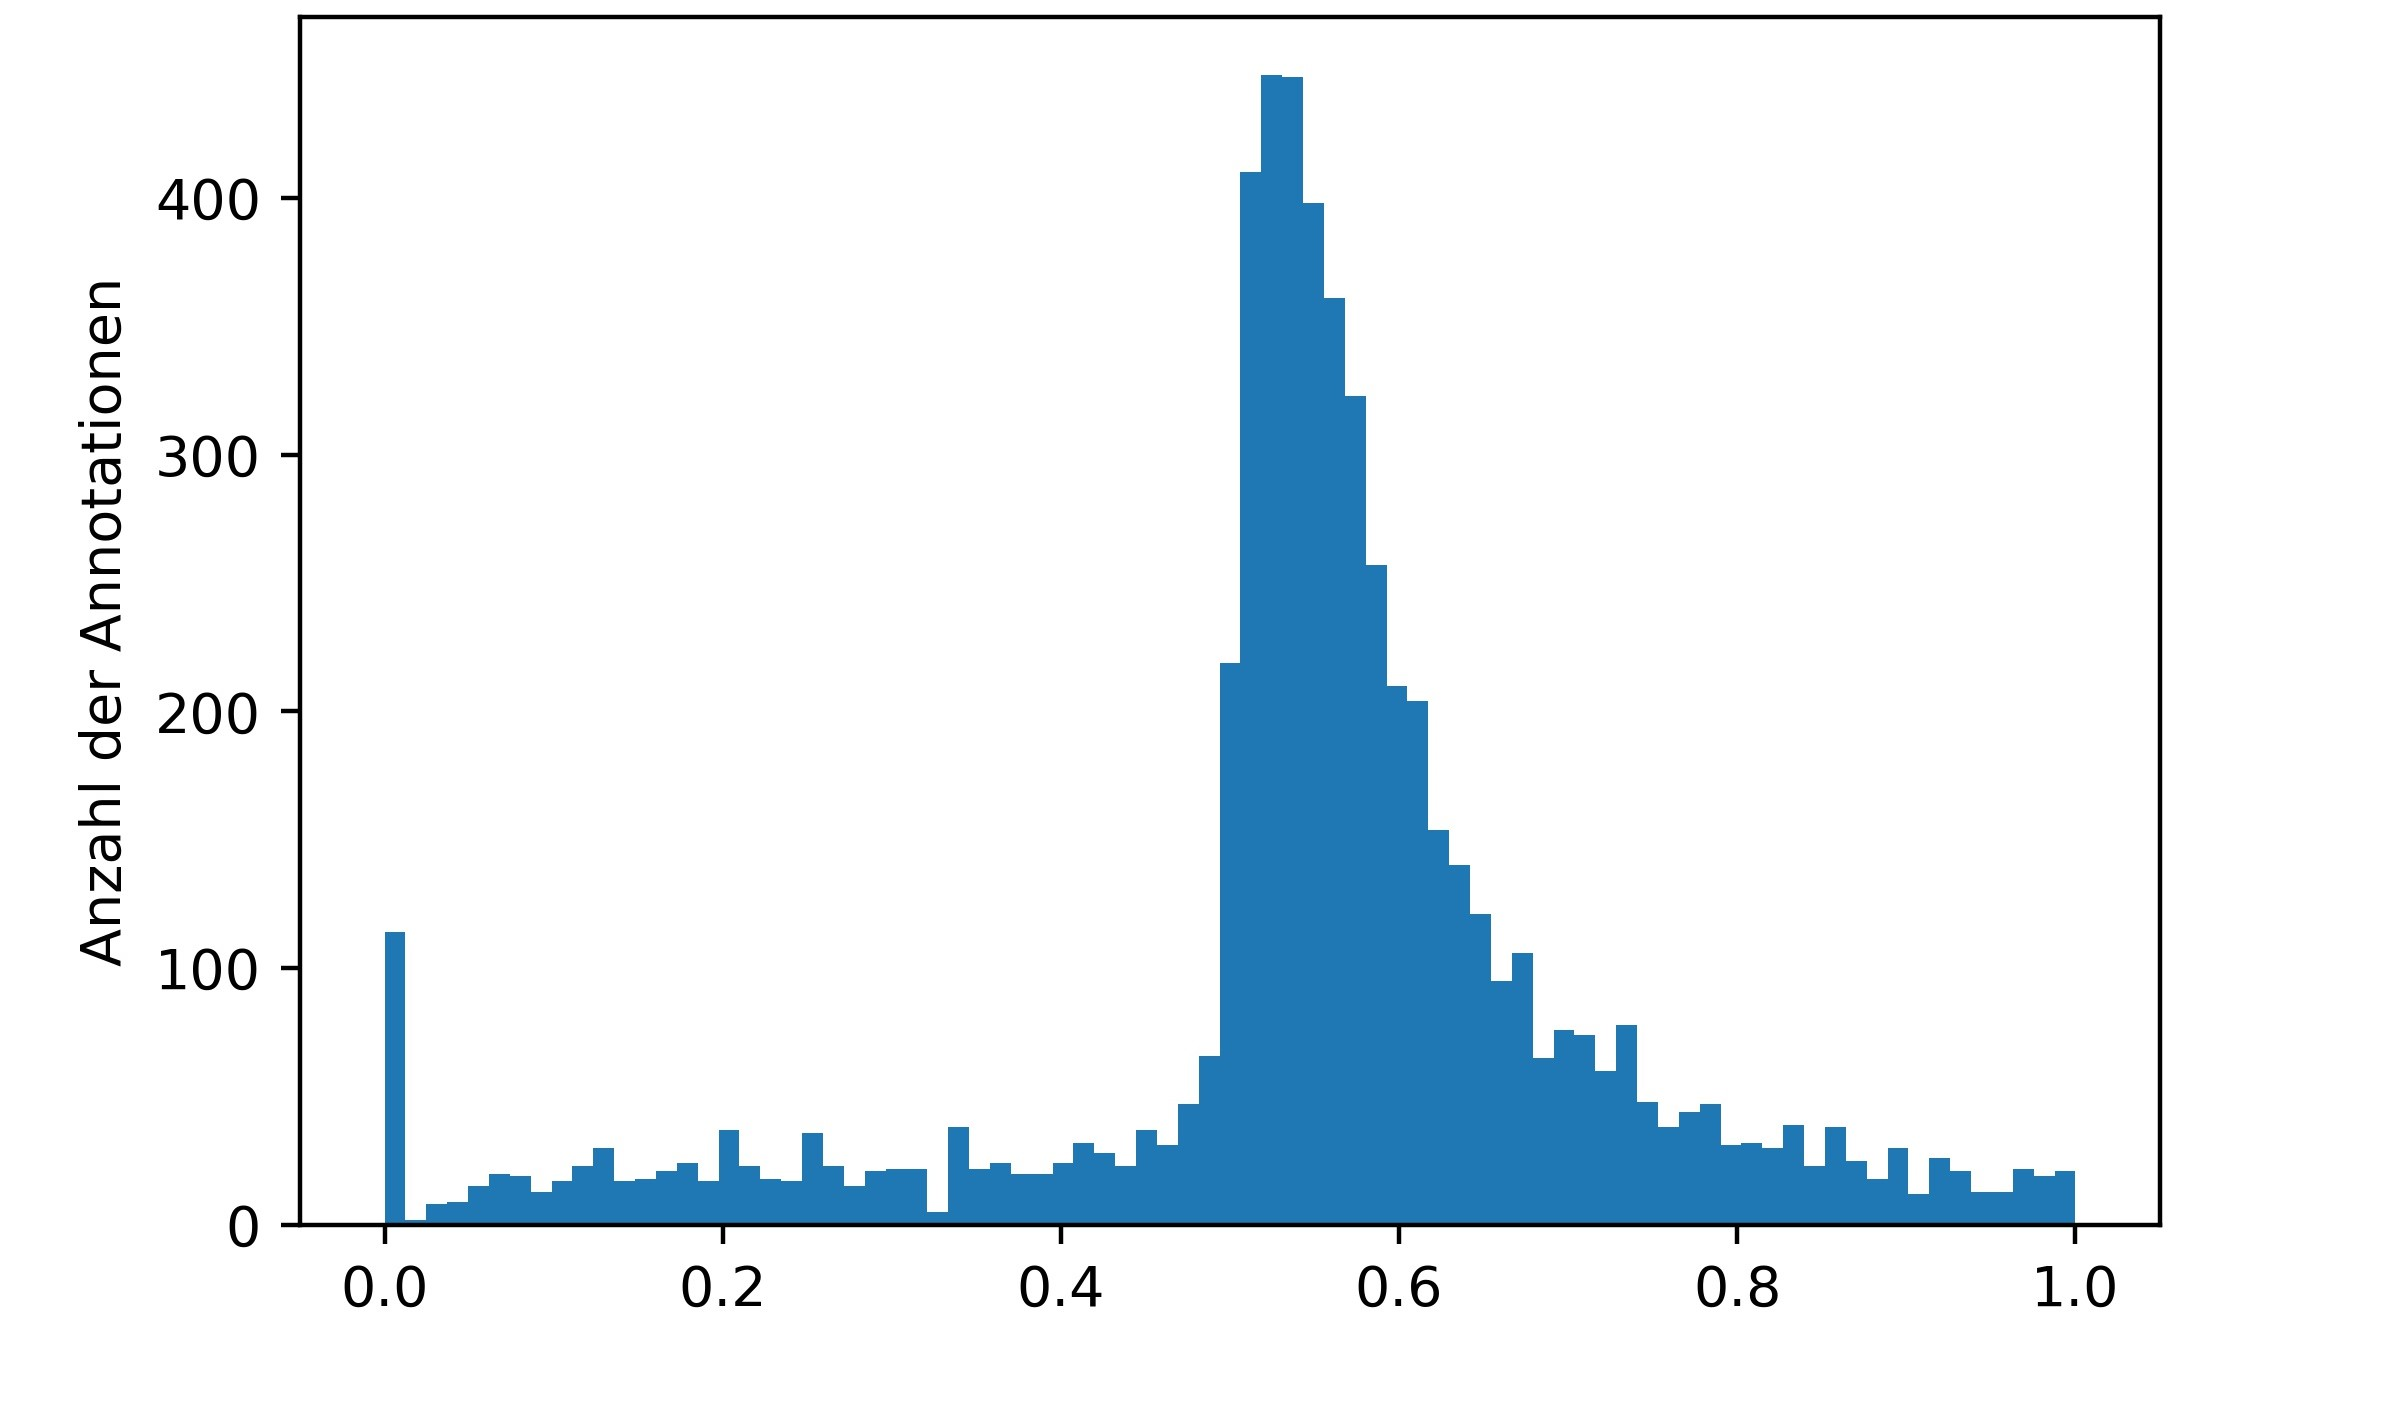
\includegraphics[width=0.80\textwidth]{./Bilder/falsch positiv Rate.jpg}
	\end{center}
	\caption{Histogramm über die falsch-positiv Rate. Die Breite der Balken wurde automatisch erstellt.}%
	\label{fig:FPrate}%
\end{figure}
 \newpage
\chapter{Diskussion}\label{chap:Diskussion}
\section{Datensatz}

Die Analyse der Metadaten zu dem Datensatz zeigt, dass die Probanden hauptsächlich einer älteren Demographie angehören und überwiegend männlich sind. Die verfügbaren Informationen beziehen sich allerdings nur auf circa die Hälfte des gesamten Datensatzes. Es kann daher nicht exakt bestimmt werden für welche Patienten die gefundenen Ergebnisse gelten. Es wurden außerdem nur die Beinbewegungen betrachtet, die im Schlaf aufgetreten sind.

An dem gegebenen Datensatz schneidet der Detektor im Vergleich zu den Detektoren aus der Literatur relativ schlecht ab. Dies ist besonders an dem vergleichsweise kleinen Korrelationskoeffizienten des PLM-Indexes (0.48) sowie Cohens $\kappa$ (0.41) und F1-Maß (0.57) zu erkennen. Insbesondere sind diese Ergebnisse wesentlich schlechter als in der Veröffentlichung von Moore et al. \cite{Moore}, obwohl diese als Vorlage für den Detektor gedient hat.

Dies könnte durch die Abweichung in der Implementierung zu dem Detektor von Moore et al. sein (siehe \ref{chap:WahldesDetektors}). Unter der Annahme, dass nur selten LM aufgrund von atemezogenen Events gelöscht werden mussten, sollte die größte Abweichung durch die fehlende Filterung des EKG zustande kommen.

In den Abbildungen \ref{fig:EKG} und \ref{fig:detectorWorking} erhöhen die Einkopplungen das Grundrauschen auf 20-30 Millivolt. Da die Ausschläge im EMG der Beinbewegungen wesentlich höher sind, sollte diese Art von Störung nur einen geringen Einfluss haben und kann alleine die starke Abweichung nicht erklären.



\begin{figure}[!ht]%
	\begin{center}
	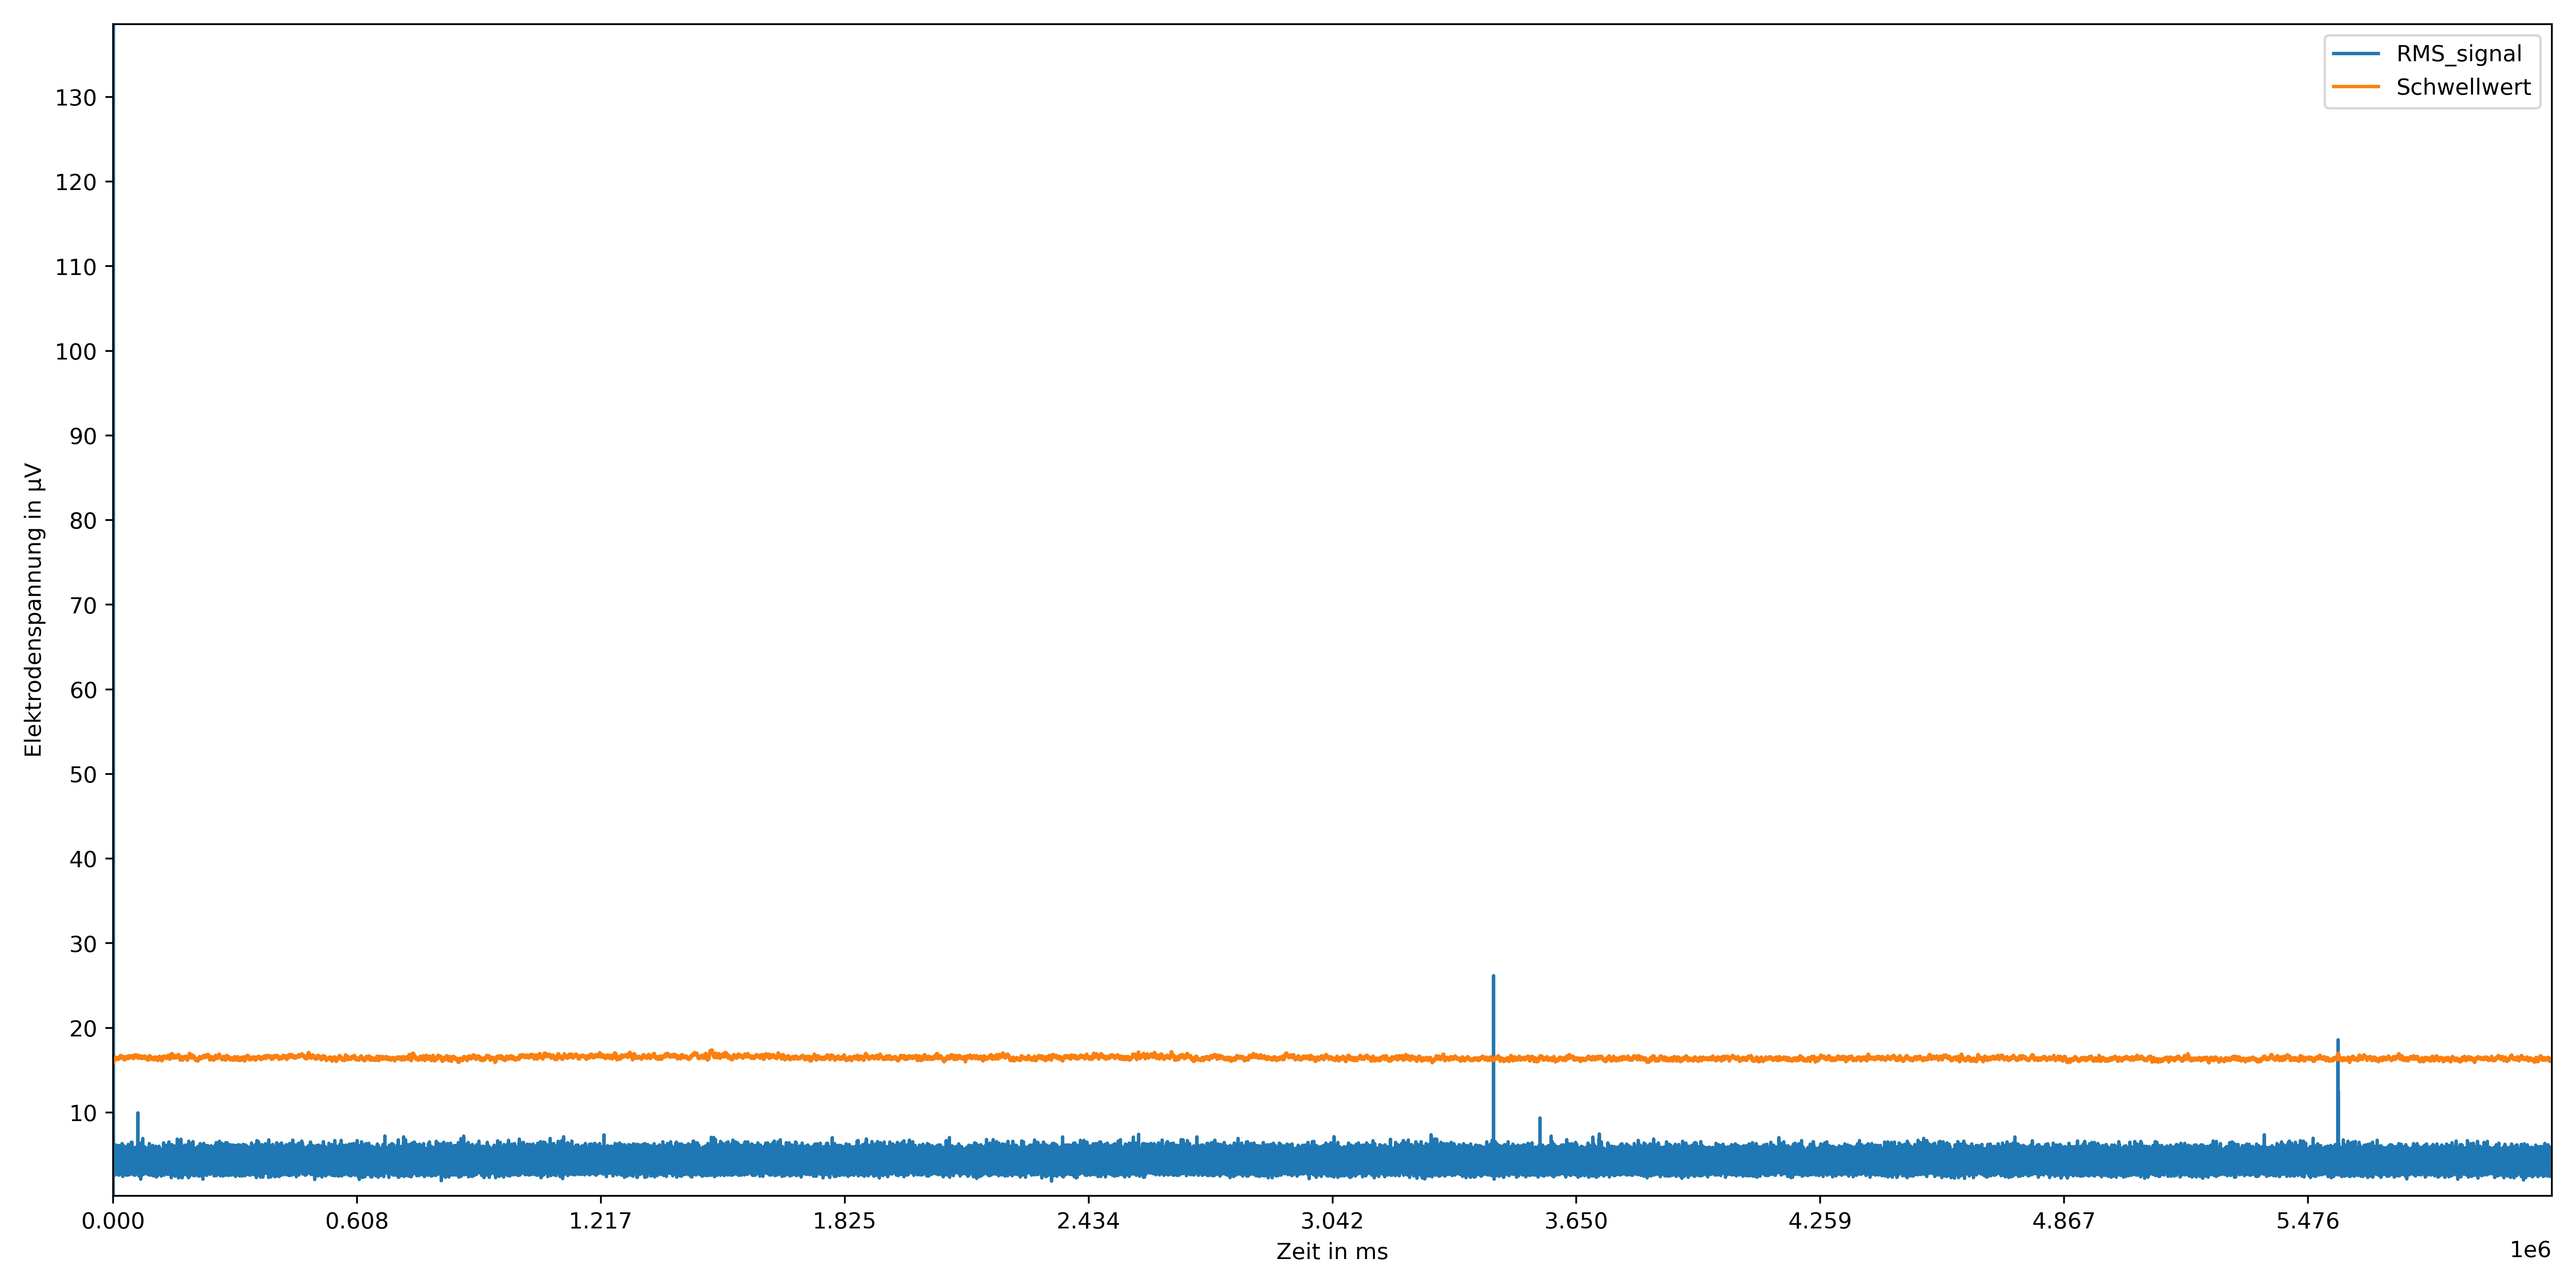
\includegraphics[width=0.80\textwidth]{./Bilder/flatSignalnohumanEMGacq_071085745.edf0,6084000.jpg}
	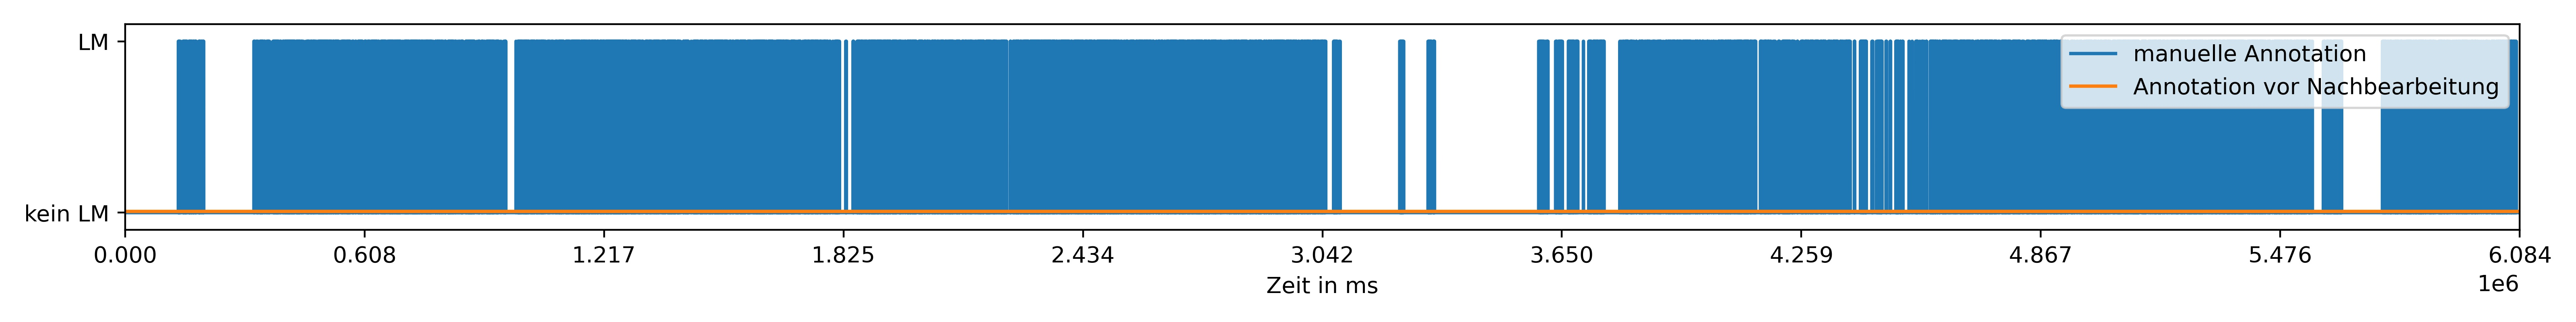
\includegraphics[width=0.80\textwidth]{./Bilder/flatSignalnohuman2acq_071085745.edf0,6084000.jpg}
	\end{center}
	\caption{Beispiel EMG-Signal mit Schwellwert (oben) und Annotationspaar (unten), bei der augenscheinlich keine Beinbewegungen stattgefunden haben. Die manuelle Annotation weist trotzdem viele Events auf.}%
	\label{fig:flat}%
\end{figure}



\begin{figure}[!ht]%
	\begin{center}
	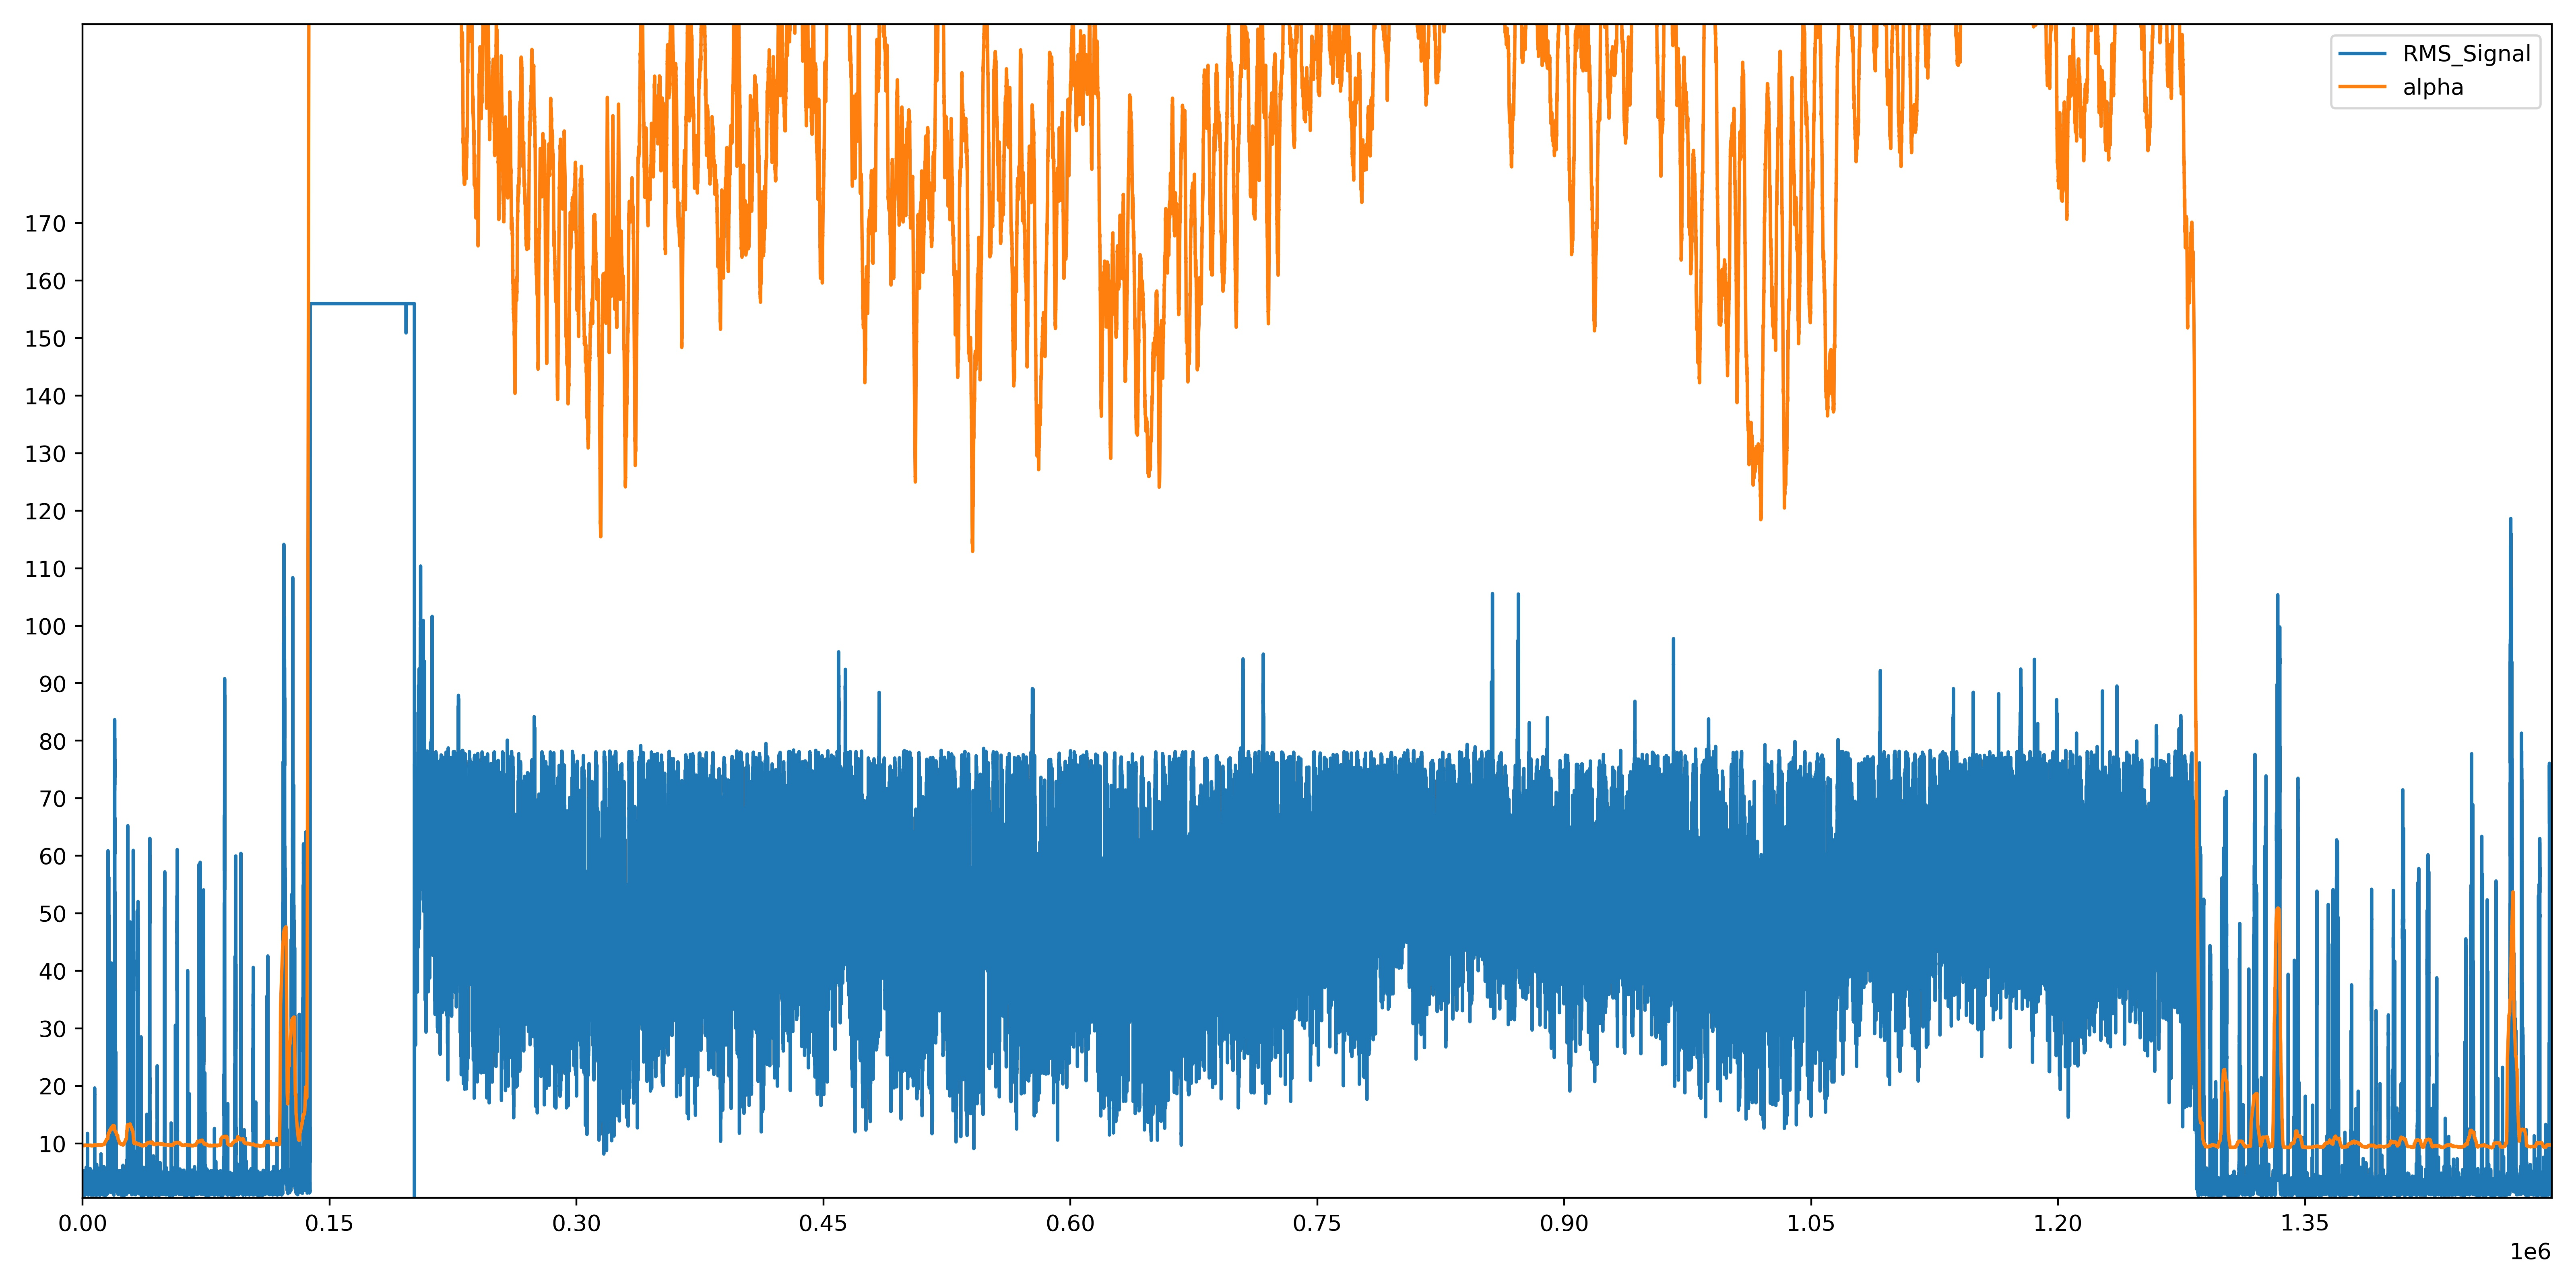
\includegraphics[width=0.80\textwidth]{./Bilder/badData1EMGacq_000952490.edf4000000,1500000.jpg}
	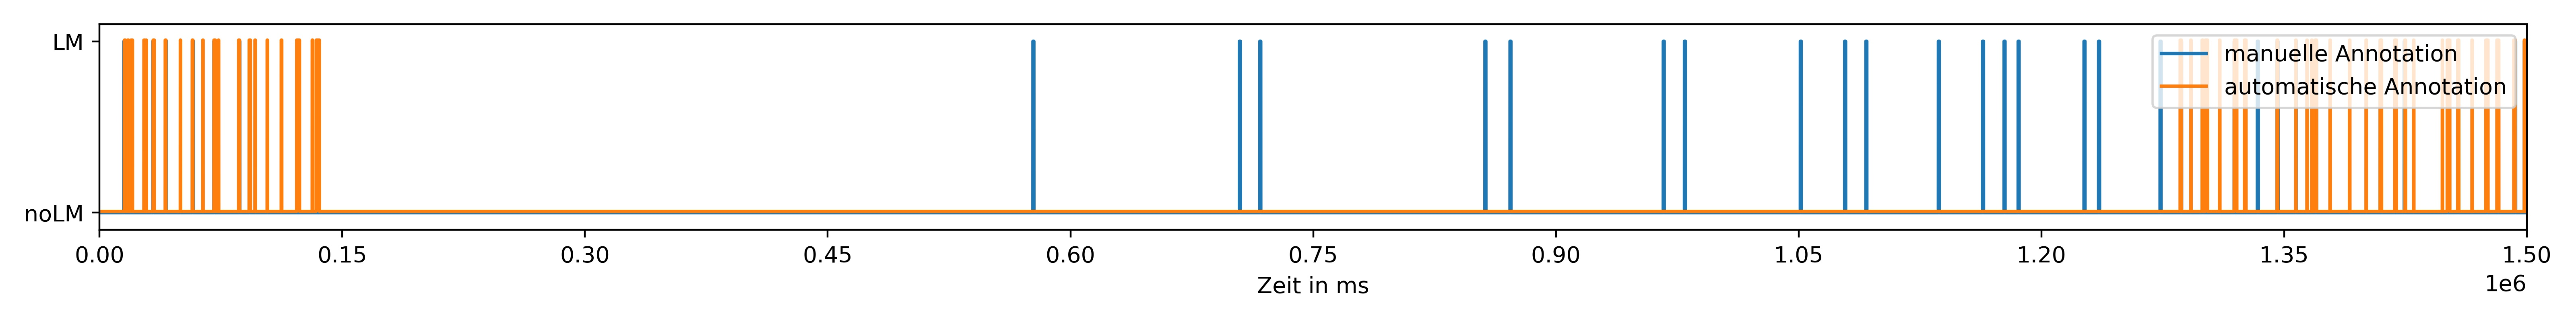
\includegraphics[width=0.80\textwidth]{./Bilder/badData1acq_000952490.edf4000000,1500000.jpg}
	\end{center}
	\caption{Ausschnitt eines EMG-Signals mit zeitweise schlechter Signalqualität (oben); laut manueller Annotation wurden in diesem Bereich trotzdem LMs gefunden (unten)}%
	\label{fig:Signalquali}%
\end{figure}

In der Abbildung \ref{fig:flat} ist ein EMG-Signal zu sehen, welches keine nenneswerten Ausschläge aufgezeichenet hat.
Die manuelle Annotation erkennt in diesem Signal sehr viele Events und es ist zu vermuten, dass das Signal von einer Annotationsunterstützung erstellt und nicht von Schlafspezialisten begutachtet wurde, bevor es in den Datensatz aufgenommen wurde.
Das Beispiel in Abbildung \ref{fig:Signalquali} zeigt eine zeitlich begrenzte Verschlechterung der Signalqualität, welche von dem dynamischen Schwellwert erkannt wird.
Zu beachten ist, dass die manuelle Annnotation in diesem Zeitraum Events aufweist.
Wahrscheinlich war nicht für alle Patienten eine explizite Untersuchung auf Beinbewegungen indiziert, sodass die Annotation möglicherweise nicht immer von Schlafspezialisten überprüft wurde. Die manuelle Annotation wurde vermutlich in diesen Fällen von einer Annotationsunterstützung erstellt.
Der Detektor wird in diesen Fällen auch an der manuellen Annotation bewertet und erzielt damit wesentlich schlechtere Ergebnisse. Die Grenzfälle mit einer sehr großen Abweichung zwischen manueller und automatischer Annotation beeinflussen den Mittelwert stark.
Die hier erzeugten Ergebnisse erlauben somit keinen Vergleich mit Detektoren, die auf anderen Datensätzen angewendet wurden.

Um die Qualtität des Datensatzes zu verbessern, empfiehlt die AASM für die Schwellwertklassifikation mit $8 \mu V$ und $2 \mu V$ Schwellwerten ein Ruhe-EMG-Signal dessen Amplitude kleiner als $\pm 10 \mu V_{pp}$. Da hier in dem gewählten Detektor ein dynamischer Schwellwert genutzt wird, kann für diese Arbeit nicht definiert werden ab welcher Grundrauschamplitude Signale ausgeschlossen werden können.


Selbst bei einem hochqualitativen Datensatz kann die manuelle Annotation von der Wirklichkeit abweichen. In der Veröffentlichung von Wetter et al. wird die Sensitivität zwischen zwei menschlichen Experten mit 97\% und die Präzision mit nur 92\% angegeben. Diese Abweichung ist für die Bewertung eines Detektors kritisch, da selbst ein hypothetisch perfekt funktionierender Detektor keine perfekten Ergebnisse hervorbringen würde. 
In Huang et al. wurde der Datensatz zusätzlich von Schlafexperten mit jahrelanger Erfahrung ausgewertet und hat somit zu einer besseren Bewertung des Detektors geführt (87.7\% im Vergleich zu 94.4\% Übereinstimmung). Bei Carvelli et al. wurde ein Konsens aus mehreren Schlafspezialisten durchgeführt um die Wirklichkeit zu approximieren. 
Diese Optionen waren für den gegebenen Datensatz nicht vorhanden. 
Da die Detektoren nur untereinander verglichen werden müssen reicht es aus die gleichen Ausgangsbedingungen für die Detektoren zu schaffen. Um die gleichen Bedingungen herzustellen sollten Detektoren nur vergleichen werden, wenn sie auf dem gleichen Datensatz getestet wurden.
Dies wird deutlich in dem Vergleich der Ergebnisse des Detektors von Moore et al., welcher auf den Daten von Alvarez-Estevez wesentlich schlechtere Ergebnisse liefert obwohl der gleiche Algorithmus verwendet wurde.


\section{Kostenfunktional}

Dass das Kostenfunktional nur sehr schwach mit den klassischen Metriken korreliert, ist damit zu begründen, dass die Ergebnisse des hier implementierten Detektors stark von den manuellen Annotationen abweichen. Dies ist insbesondere an dem kleinen Korrelationskoeffizienten der PLM-Indices zu erkennen.

Ein Problem bei der eventweisen Klassifikation ist, dass ein Abtastwert den Unterschied in der Anzahl der LM bedeuten kann. Da die Entscheidung welche der LM einander zugeordnet werden intuitiv von der Umgebung abhängt, ist es nicht einfach Regeln zu definieren, wann ein TP gezählt werden sollte.

Beim Bewerten des Detektors wurden Fehler ausschließlich anhand des binären Annotationssignals ohne vertiefende Fachkenntnis eines Schlafspezialisten definiert. Diese hätten möglicherweise bestimmte Fehler anders beurteilt, sodass sie in dem medizinischen Kontext ein aussagekräftigeres Ergebnis lieferten. 

Aufgrund der Definition der Güte \ref{Güte} der relativen Kosten kommt es außerdem zu einer Verzerrung der Interpretation bei gut funktionierenden Detektoren. Falls die relativen Kosten sehr klein sind und die Differenz der relativen Kosten zweier Detektoren relativ klein ist, wird es aufgrund der Nichtlinearität der Güte zu einem unerwartet großen Unterschied kommen. Die Güte ist also für kleine Kosten schlechter konditioniert. Das hat aber zusätzlich den Vorteil, dass sehr ähnliche Detektoren gut voneinander getrennt werden können.

Aufgrund dessen, dass für das Kostenfunktional Fehler gezählt werden, gibt es keine Obergrenze die der Wert annehmen kann. Die untere Grenze liegt bei Null. Das bedeutet auch, dass die Güte (zumindest bei unendlicher Signallänge) unendlich sein kann, wenn keine Fehler gemacht werden. 
Falls manuell keine PLM-Serien erkannt werden, sind die relativen Kosten wenig aussagekräftig, und gehen gegen unendlich, auch wenn nur ein Fehler gemacht wird. Wenn zusätzlich keine PLM-Serien vom Detektor erkannt werden, sind Kosten und Güte nicht definiert. Signale ohne manuelle Annotation sollten aus diesem Grund nicht zur Bewertung verwendet werden. 

Ein weiteres Problem ist, dass es bei einer PLM-Serie mehrere Gründe geben kann, warum diese fehlerhaft sind. So kann es beispielsweise dazu kommen, dass der erste TP eines 1toX-Matchings (welches die Serie verändert) gleichzeitig fälschlicherweise die [5-90] Sekunden Intervallgrenze überschreitet. 
Diese Fehler werden in der Aufschlüsselung der Kosten bei beiden Gründen sichtbar. Im Kostenfunktional wird in solchen Fällen nur ein Fehler gezählt.
Das Problem mit der Berechnung des Kostenfunktionals ist, dass es möglicherweise noch wesentlich mehr Grenzfälle gibt, als in dem in dieser Arbeit in Betracht gezogen wurden. Es eignet sich hierfür eine Implementierung, bei der für jedes LM die Gründe für die Fehler analysiert werden, anstatt für jeden Fehlergrund die LM zu suchen, die dagegen verstoßen.

Die Formel \ref{kdiff} $$
\overset{\text{ergebniserhöhende Fehler \textminus \ ergebnisverkleinernde Fehler}}{\underset{\text{automatisch annotierte PLM \textminus \ manuell annotierte PLM}}{=}}
$$
beschreibt inwieweit die Fehler, die von dem Detektor verursacht wurden, (PLM Differenz) von dem Kostenfunktional (Differenz aus Zuvielzählen und Zuwenigzählen) erklärt werden können. 
Da diese beiden Differenzen stark korreliert sind ($r^{2} = 0.99 $), kann geschlussfolgert werden, dass Kostenfunktional eine zuverlässige Beschreibung der Güte des Detektors ist.
Die weitere Untersuchung auf unbekannte Grenzfälle vernachlässigt werden, da diese das Ergebnis nur wenig beeinflussen.

Das Kostenfunktional ist auf die Kriterien der AASM zur Erkennung von PLM spezialisiert und kann deswegen auch nur in diesem Rahmen angewandt werden. Sollten sich diese Regeln ändern oder wird ein anderes Regelwerk bevorzugt, müssen die hier vorgeschlagenen Berechnungen angepasst werden und es lassen sich somit auch keine Vergleiche mehr zwischen den Bewertungen vor dieser Regeländerung herstellen. 
Die Prinzipien, für die Erstellung des Kostenfunktionals können auf ähnliche regelbasierte medizinische Fragestellungen angewandt werden. 


\section{Verbesserung der Einordnung des Detektors}
Da einige Gründe bekannt sind, aus denen die manuelle Annotation fehlerhaft sein könnte, bietet es sich an, die erhobenen Metriken aus dem Kapitel Verbesserung der Einordnung  des Detektors (Kapitel \ref{Verbesserung}) zu nutzen, um die Qualität des Datensatzes zu verbessern. 
Im Folgenden sind einige dieser Gründe aufgezählt und interpretiert.
Zuerst kann die Annahme getroffen werden, dass der Detektor seine Annotationsentscheidungen nur anhand der vorliegenden Daten trifft. Bei einer manuellen Annotation können andere Faktoren wie Monotoniemüdigkeit (siehe \ref{chap:Einleitung}) eine Rolle spielen. Sind beispielsweise Annotationspaare vorhanden, bei denen die manuelle Annotation ausschließlich im vorderen Teil der Nacht befinden, während automatische Annotationen über die ganze Nacht verteilt sind, könnte das bedeuten, dass die manuelle Annotation aus unbekannten Gründen abgebrochen wurde.

Die Teilmenge an Daten die vorzeitig abgebrochen wurde, weist tendenziell eine größere Abweichung der Schwerpunktdifferenz auf. Ein Extrembeispiel dafür könnte in Abbildung \ref{fig:noisy} zu sehen sein. Hier könnte die hohe Eventdichte für einen frühzeitigen Abbruch der manuellen Annotation geführt haben. Die Schwerpunktdifferenz liegt in dem folgenden Beispiel bei 3.03 Stunden.


\begin{figure}[!ht]%
	\begin{center}
	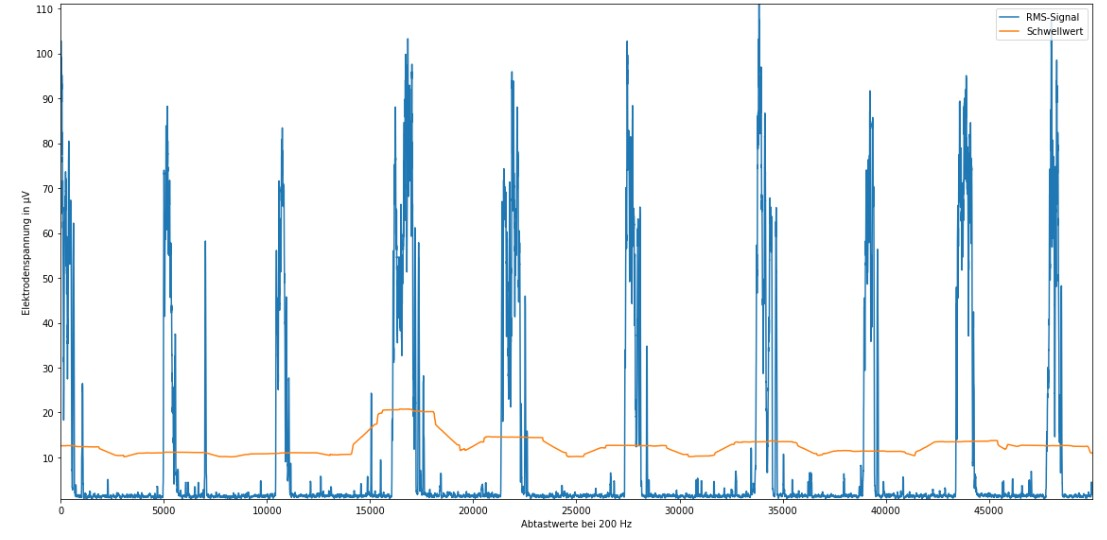
\includegraphics[width=0.80\textwidth]{./Bilder/starkesRauschenzoomedEMGacq_424517352.edf0,6516000.jpg}
	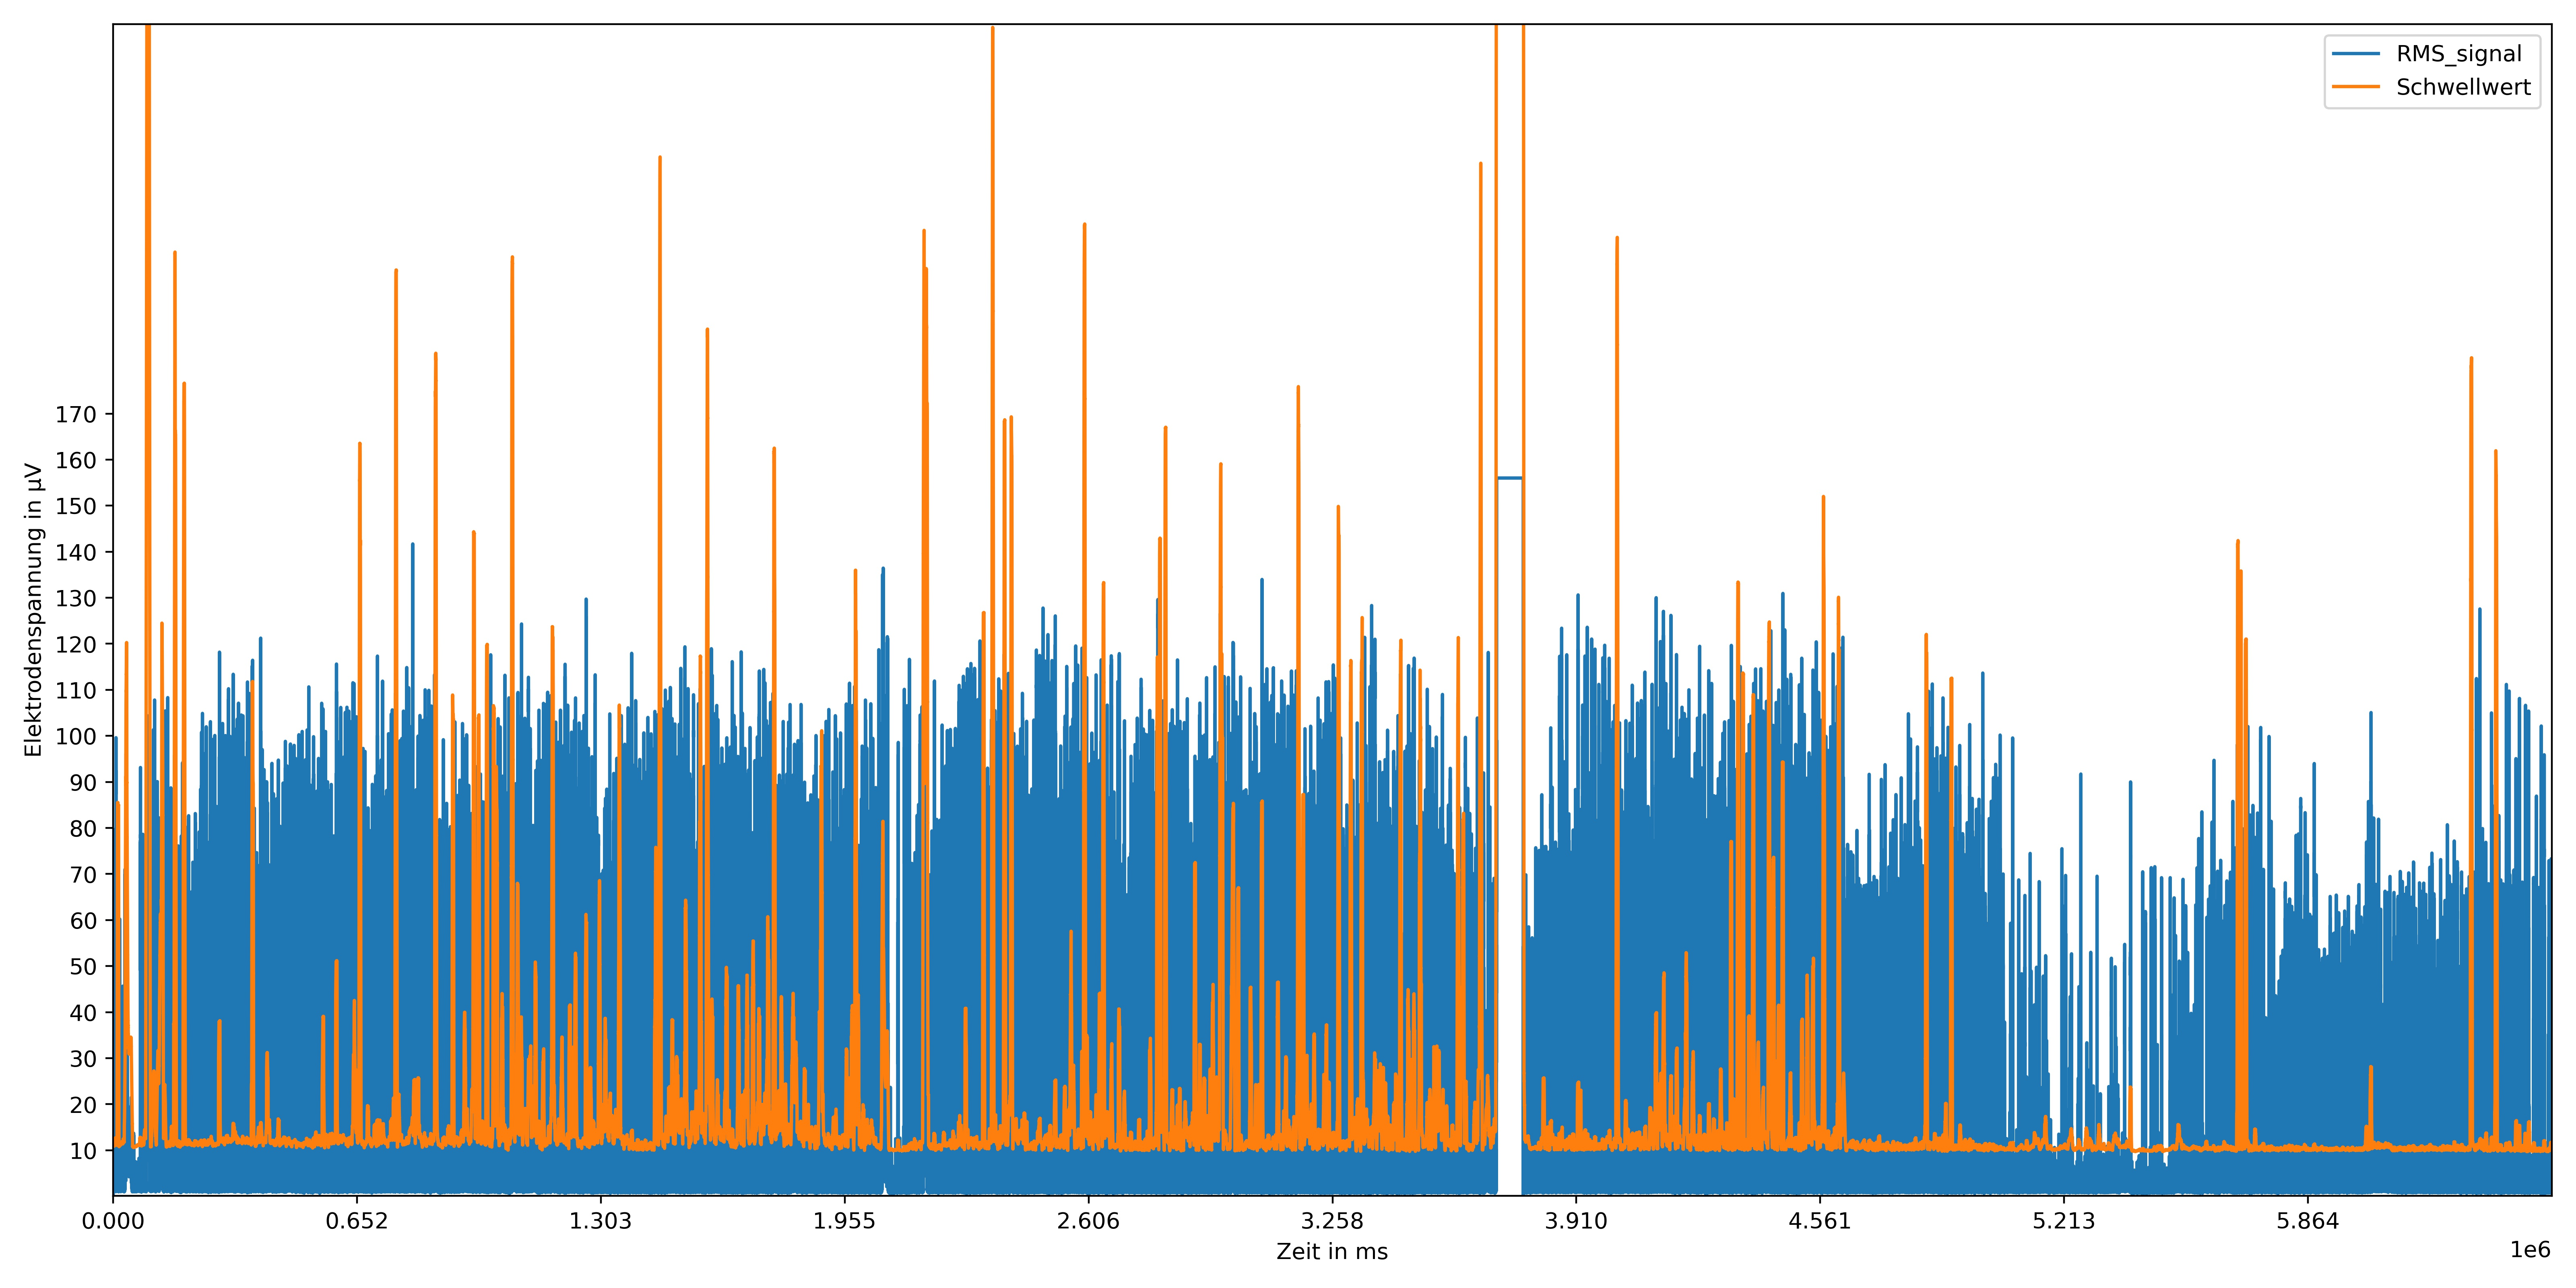
\includegraphics[width=0.80\textwidth]{./Bilder/starkesRauschenEMGacq_424517352.edf0,6516000.jpg}	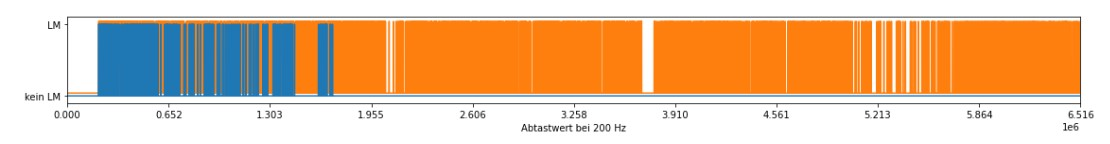
\includegraphics[width=0.80\textwidth]{./Bilder/starkesRauschen2acq_424517352.edf0,6516000.jpg}
	\end{center}
	\caption{Ausschnitt eines EMG-Signals mit sehr hoher Eventdichte(oben); das selbe EMG-Signal über die ganze Nacht dargestellt (mittig) mit zugehörigen Annotationen (unten); welche eine hohe Schwerpunktdifferenz aufweisen.}%
	\label{fig:noisy}%
\end{figure}


Im Histogramm \ref{fig:centers} ist eine solche Teilmenge weit entfernt von dem Mittelwert. Es kann jedoch ohne medizinisches Fachwissen kein Schwellwert definiert werden, unter dem die Daten aussortiert werden könnten. 


Bei einer segmentweisen manuellen Annotation wird der tatsächliche Startzeitpunkt in die Segmente diskretisiert. Da die meisten Detektoren quasizeitkontinuierlich auswertet, kann dieser bei ausreichend guter Detektionsqualität die Wirklichkeit zeitlich genauer darstellen. 
Gäbe es beispielsweise einen ungenau annotierenden Angestellten, der jede echte Beinbewegung eine Sekunde vorher (gerundet auf die Segmentgrenzen) schon als positiv markiert, würde der daraus resultierende Mittelwert der Startzeitpunkte über diese Nacht gesehen einen Ausreißer im Histogramm produzieren.
Diese Metrik könnte also einen Hinweis darauf geben, welche Dateien genauer untersucht werden sollten.
Es könnte argumentiert werden, dass Annotationen, welche im Mittel ungenauer sind als die Segmentgrenzen es zulassen, eher hinderlich für die Bewertung des Detektors sind, da die Startzeitpunkte den PLM-Index direkt beeinflussen.


Die Löschung von LM, die in der Nähe von atembezogenen Events stattgefunden haben, ist beispielsweise für den Detektor, ohne die benötigten Atem-Signale nicht zu erkennen. Unter der Annahme, dass diese Art von Events nicht bei allen Patienten auftritt, könnte es sinnvoll sein, die Nächte genauer zu untersuchen, bei der die falsch positiv Rate stark von dem Mittelwert abweicht. Anhand des  Histogramms \ref{fig:FPrate} aus den Ergebnissen, ist nicht zu erkennen, ab welchem Wert eine starke Abweichung zu vermuten ist. Diese Abweichung wird vermutlich erst bei sehr guten Ergebnissen sichtbar.


Ein sehr hohes LM Verhältnis bedeutet, dass der Detektor wesentlich öfter auf einen Anstieg im EMG-Signal reagiert als das medizinische Personal es tun würde. Diese Metrik könnte also einen Hinweis darauf geben, wie sinnvoll es ist, den Erkennungsschwellwert anzuheben. Die Aussage des Mittelwertes und des Medians ist für den implementierten Detektor widersprüchlich. Betrachtet man das die Differenz der gefundenen LM (automatisch gefundene LM – manuell gefundene LM) wird ersichtlich, dass der Detektor in den meisten Fällen weniger LM als das medizinische Personal erkennt. Im Durchschnitt erkennt der Detektor 87.1 von 226 Beinbewegungen zu wenig. In diesem Fall könnte also die Formel für den Schwellwert angepasst werden, sodass mehr LM erkannt werden. 



Eine hohe Anzahl an 1toX-Matches impliziert, dass der Detektor das Ende eines LM zu früh erkennt. In diesen Fällen könnte beispielsweise eine Änderung in den Zeiten der Nachbearbeitung des Annotationssignals oder die Definition des unteren Schwellwertes angepasst werden. Die Anzahl der Xto1-Matches trifft entgegengesetzte Aussagen. In dem hier implementierten Detektor sind beide Anzahlen nicht besonders hoch.
Falls es Verstöße gegen die definierte Länge der LM gibt, könnte das bedeuten, dass der Detektor entweder Ausschläge im EMG als LM klassifiziert, die nicht aus Beinbewegungen stammen oder die Dauer eines richtig gefundenen LM wird falsch eingeschätzt. Diese Metrik ist für den Detektor per Definition bei Null, da in der Nachbearbeitung des Annotationssignals die Länge der gefundenen LM überprüft wird.


Die Mittelwerte der Verteilung (über alle Nächte berechnet) kann genutzt werden, um den Detektor auf systematische Fehler zu untersuchen. Liegen beide Mittelwerte bezogen auf die manuelle Annotation zeitlich gesehen im positiven Bereich, kann das darauf hindeuten, dass die Vorverarbeitung des EMG-Signals einen zu starken Tiefpasscharakter aufweist und somit die Flanken der LM weniger schnell ansteigen und abfallen. Dies würde dazu führen, dass alle automatisch erkannten LM leicht zeitlich versetzt zu den korrespondierenden manuell erkannten LM sind.
Es ist zu vermuten, dass in der manuellen Annotation auch systematische Fehler gemacht wurden. Da die Mittelwerte der Startzeitpunkte negativ und die Mittelwerte der Endzeitpunkte positiv sind, lässt sich vermuten, dass das medizinische Personal, anstatt exakt ab- und aufzurunden, lieber das ganze Segment als positiv definiert hat, in dem ein LM stattgefunden hat.
Aus diesem Grund können systematische Fehler nur zwischen den Detektoren untereinander verglichen werden.

Maschinelle Lernalgorithmen sind aufgrund der hohen Anzahl der Parameter in der Lage sich an den Trainingsdatensatz stark anzupassen. Es kann also passieren, dass der Algorithmus die Segmentierung der Annotation mitlernt, obwohl diese in dem Eingangssignal nicht vorhanden sind.
Die Verteilung der LM-Startzeitpunkte hat aufgrund der Segmentierung der manuellen Annotation eine bestimmte Standardabweichung. Wird von einem Detektor, der mithilfe eines solchen Lernalgorithmusses arbeitet diese Standardabweichung unterschritten, könnte eine Überanpassung an die Segmentgrenzen stattgefunden haben. Diese Überanpassung lässt sich anhand dieser Metrik feststellen. 
Ein Neuronales Netz welches die Segmentgrenzen auswendig gelernt hat, würde auf einem anderen Datensatz mit quasikontinulierlicher manueller Annotation eine unerwartet hohe Standardabweichung aufweisen und damit auch zu schlechteren Ergebnissen führen. Die Struktur eines Schwellwertdetektor hat zu wenig wählbare Parameter um Segmentgrenzen zu erlernen. Daher kann die Metrik hier nicht ausgewertet werden.



\section{Optimierung des Detektors}

Es sollte darauf geachtet werden, dass die Bewertung des Detektors nicht mit der Optimierung des Detektors vermischt wird. Da die Optimierung anhand der Metriken im Kapitel Verbesserung der Einordnung des Detektors (Kap. \ref{Verbesserung}) unabhängig von dem Kostenfunktional ist, können diese genutzt werden. 
Es wird trotzdem empfohlen die Bewertung des Detektors anhand von Daten durchzuführen, die nicht zu einer Veränderung des Detektors geführt haben.
Das Kostenfunktional lässt sich durch die Zählweise nicht mathematisch ableiten und kann somit nicht durch Optimierungsverfahren genutzt werden, die auf Gradienten beruhen. Trotzdem lassen sich Detektoren aufgrund der Definition einer Güte, welche als Inverse der Kosten definiert ist, durch Verfahren wie genetischen Algorithmen verbessern. \newpage
\chapter{Fazit und Ausblick}\label{chap:Fazit_und_Ausblick}

Aus der vorliegenden Arbeit ging hervor, dass die klassischen Metriken ungeeignet für die Bewertung der Eventdetektoren im Kontext der periodischen Beinbewegungen sind. Diese sind insbesondere ungeeignet, da wichtige Informationen über zeitliche Zusammenhänge verloren gehen, Metriken sich untereinander qualitativ widersprechen können und auch mit trivialen Detektoren perfekte Ergebnisse erzielt werden können.

Es wurde daher ein Kostenfunktional vorgestellt, welches auf dem medizinisch relevanten PLM-Index basiert und die Fehler, die vom Detektor verursacht wurden, quantifiziert darstellt. Die aufgetretenen Fehler konnten sehr gut ($r^{2} = 0.99$) durch das Kostenfunktional erklärt werden. Durch dieses Vorgehen wird eine einfache und eindeutige Vergleichbarkeit ermöglicht, indem jedem Detektor genau ein Gütewert zugewiesen wird. 

Das vorgestellte Kostenfunktional ist besonders dann nützlich, wenn Vergleichswerte existieren, um neu entwickelte Detektoren einordnen zu können. Dafür sollte das Kostenfunktional in zukünftigen Arbeiten auf die bereits existierenden Detektoren angewendet werden und ein neuer Stand der Technik festgelegt werden. Für qualitative Aussagen sollte ein möglichst öffentlich zugänglicher Datensatz definiert werden, an dem alle Detektoren und Metriken angewendet werden können. Im Optimalfall hat dieser Datensatz eine gute manuelle Annotation. Primär ist jedoch wichtig, dass die Qualität des Datensatzes für alle Detektoren gleich ist, damit die Unterschiede in den Datensätzen nicht fälschlicherweise mit in die Bewertung des Detektors einfließen.


Für eine Weiterentwicklung des hier vorgestellten Kostenfunktionals sollten insbesondere Grenzfälle betrachtet werden, um herauszufinden, ob es weitere relevante Fehlerquellen gibt, bei denen der Algorithmus nicht erwartungsgemäß funktioniert. 

Die im Kapitel \ref{Verbesserung} präsentierten Ideen können genutzt werden, um einerseits einen Datensatz zu bereinigen, indem Ausreißer gefunden werden können und andererseits fundiertere Aussagen über die Funktionsweise des Detektors zuzulassen. Diese Aussagen sind jedoch nur als Hinweise zu verwenden, an welchen Stellen genauere Untersuchungen lohnenswert sind. Für den verwendeten Detektor konnten keine definitiven Aussagen getätigt werden.
Die Wirksamkeit der Ideen und die Festlegung von Schwellwerten könnte sich jedoch bei anderen Detektoren als nützlich erweisen und sollte in zukünftigen Arbeiten mithilfe von Experten durchgeführt und überprüft werden.
 \newpage

			
			
%------------ Literaturverzeichnis -------------------------------
\pagenumbering{roman}

% Der roman counter wird mit setcounter{page}{1} vor 
% Subfiles-Einbindung auf 1 zurück gesetzt, soll aber 10 sein
% um an letzte römische Nummerierung anzuschließen
\setcounter{page}{10}

\renewcommand*{\bibname}{Quellenverzeichnis}
\printbibliography
\clearpage


%------------ Anhang ---------------------------------------------
\appendix
%Abbildungsnummerierung im Format Kapitel.Nummer
% \renewcommand{\thefigure}{\Alph{chapter}.\arabic{figure}}
% \renewcommand{\thesection}{A.\arabic{section}}
%\pagenumbering{Alph}
\addchap{Anhang}
\chapter{Anhang}\label{chap:Anhang}
\begin{figure}[!ht]%
	\begin{center}
	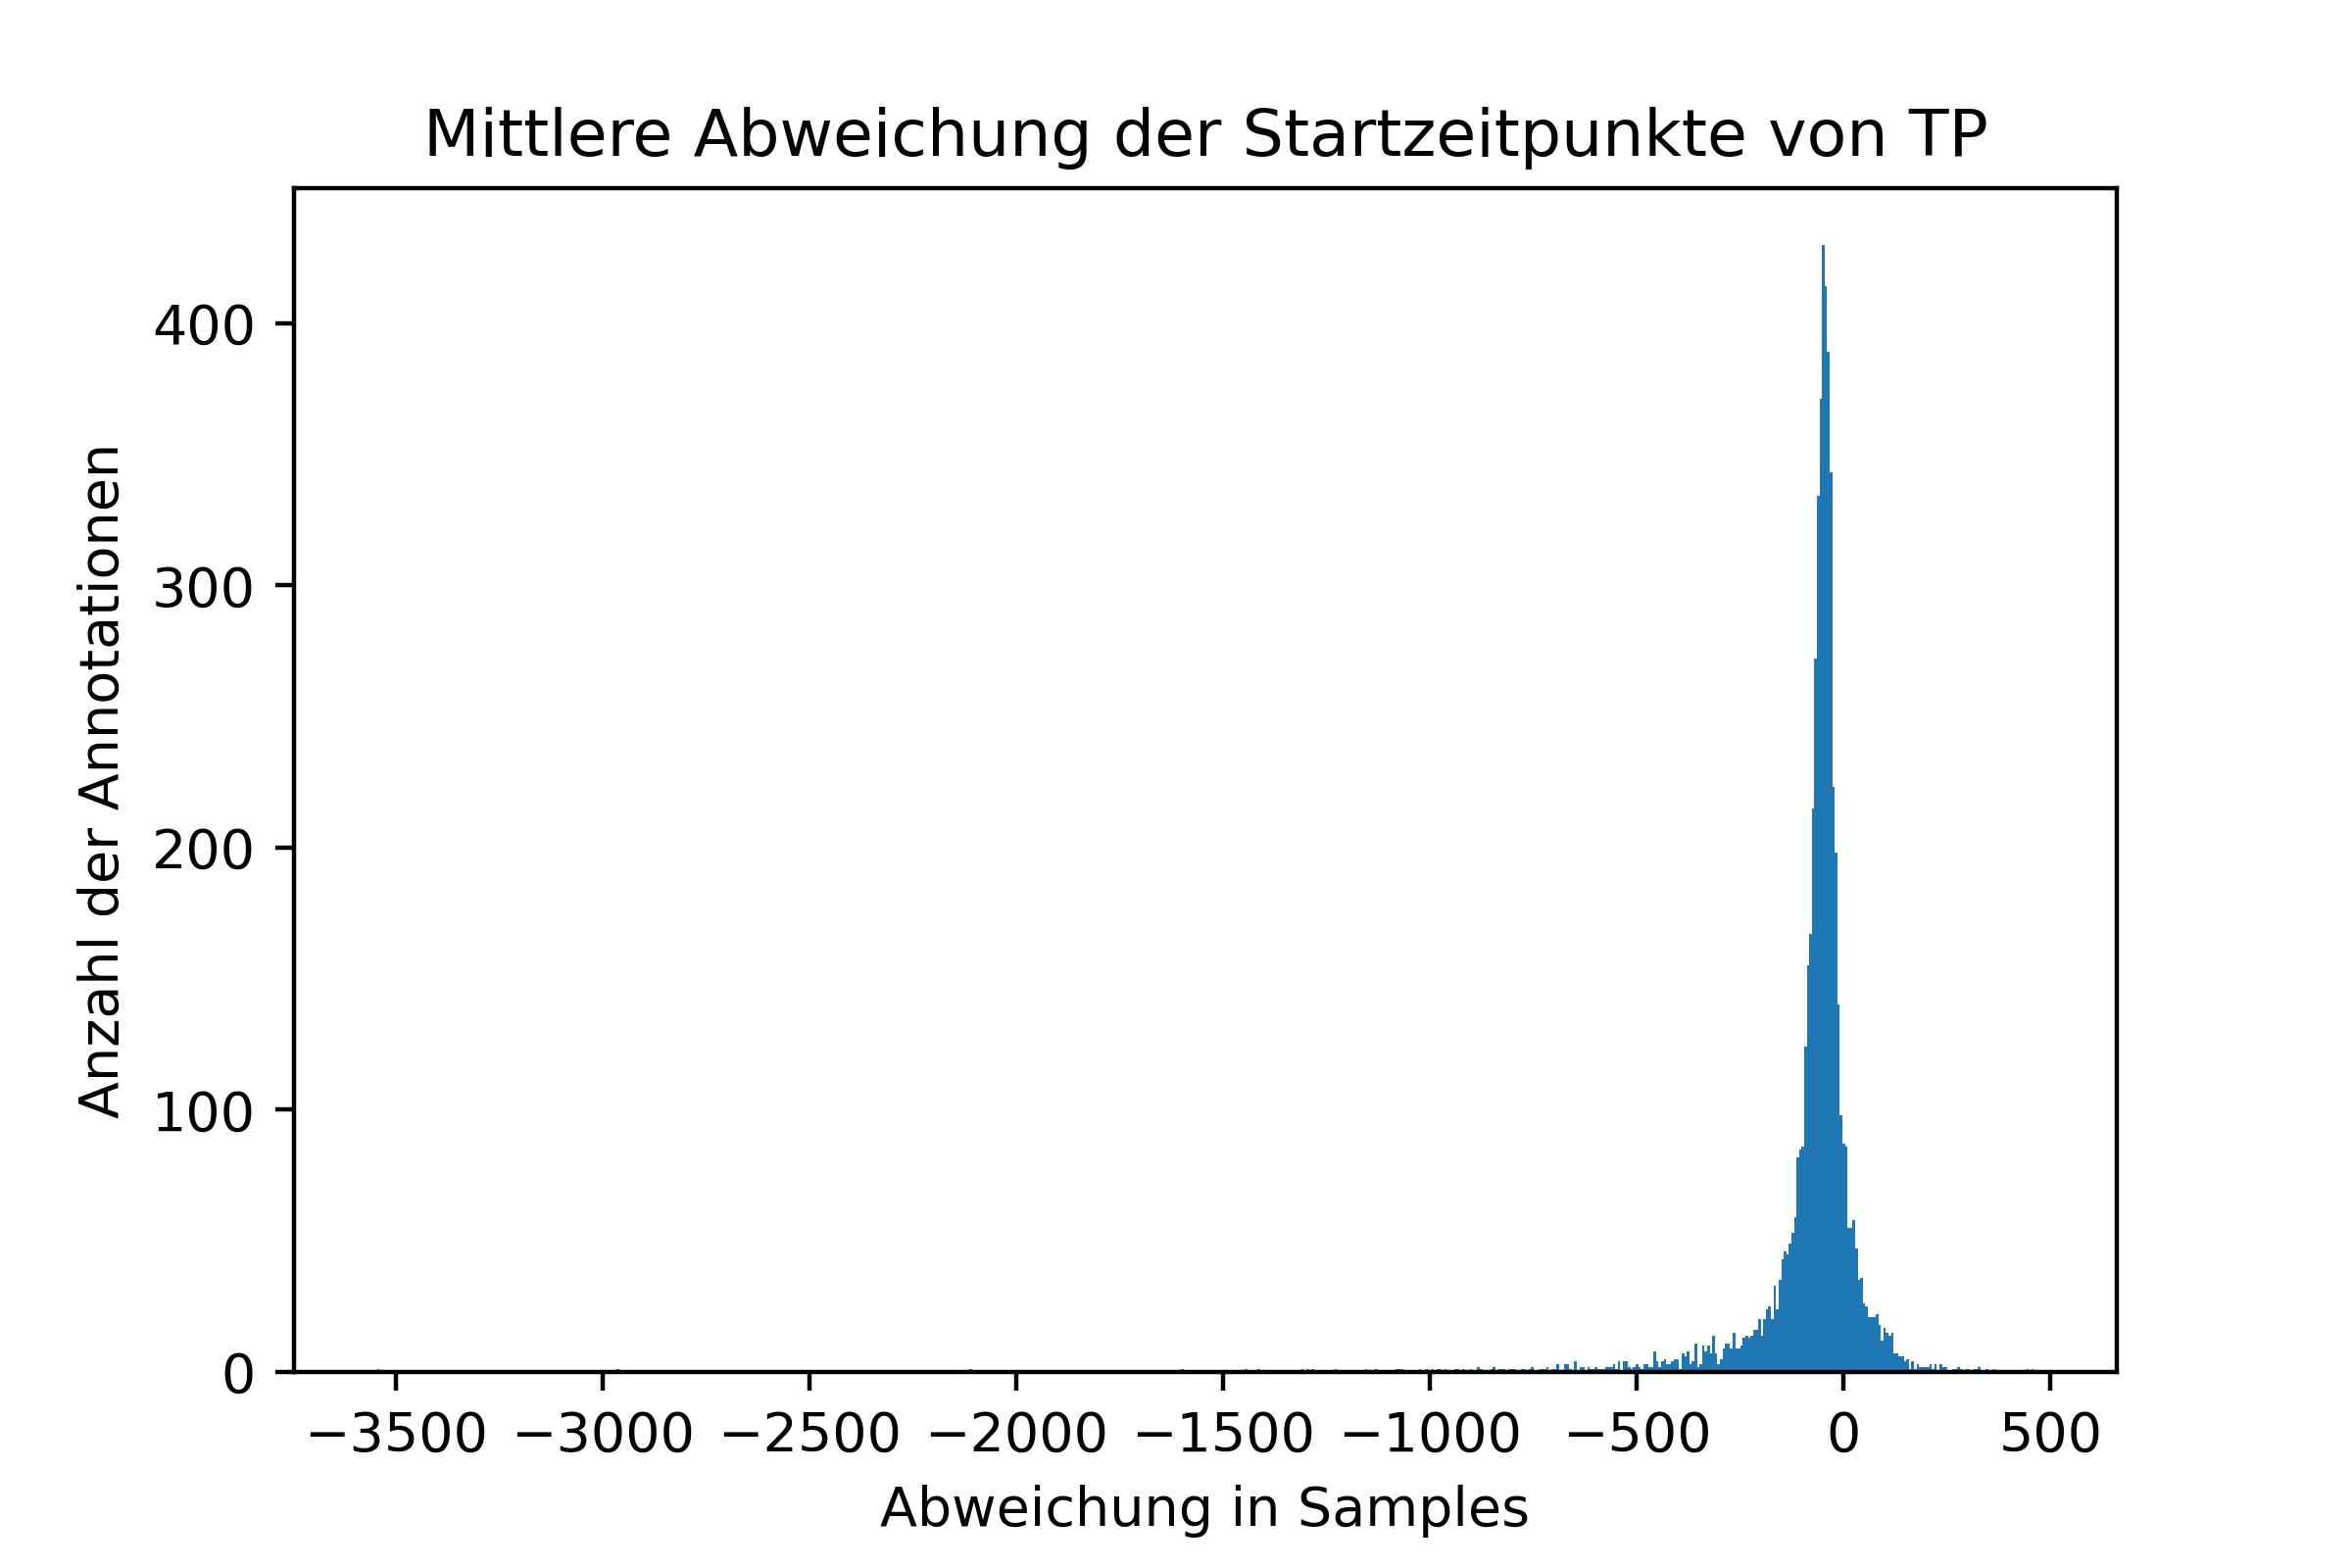
\includegraphics[width=0.80\textwidth]{./Bilder/LMStartDistribution_means.jpg}
	\end{center}
	\caption{Histogramm über die Mittlere Abweichung der Startzeitpunkte von TP bei einer Abtastfrequenz von 200 Hertz}%
	\label{fig:AASMKrit}%
\end{figure}

\begin{figure}[!ht]%
	\begin{center}
	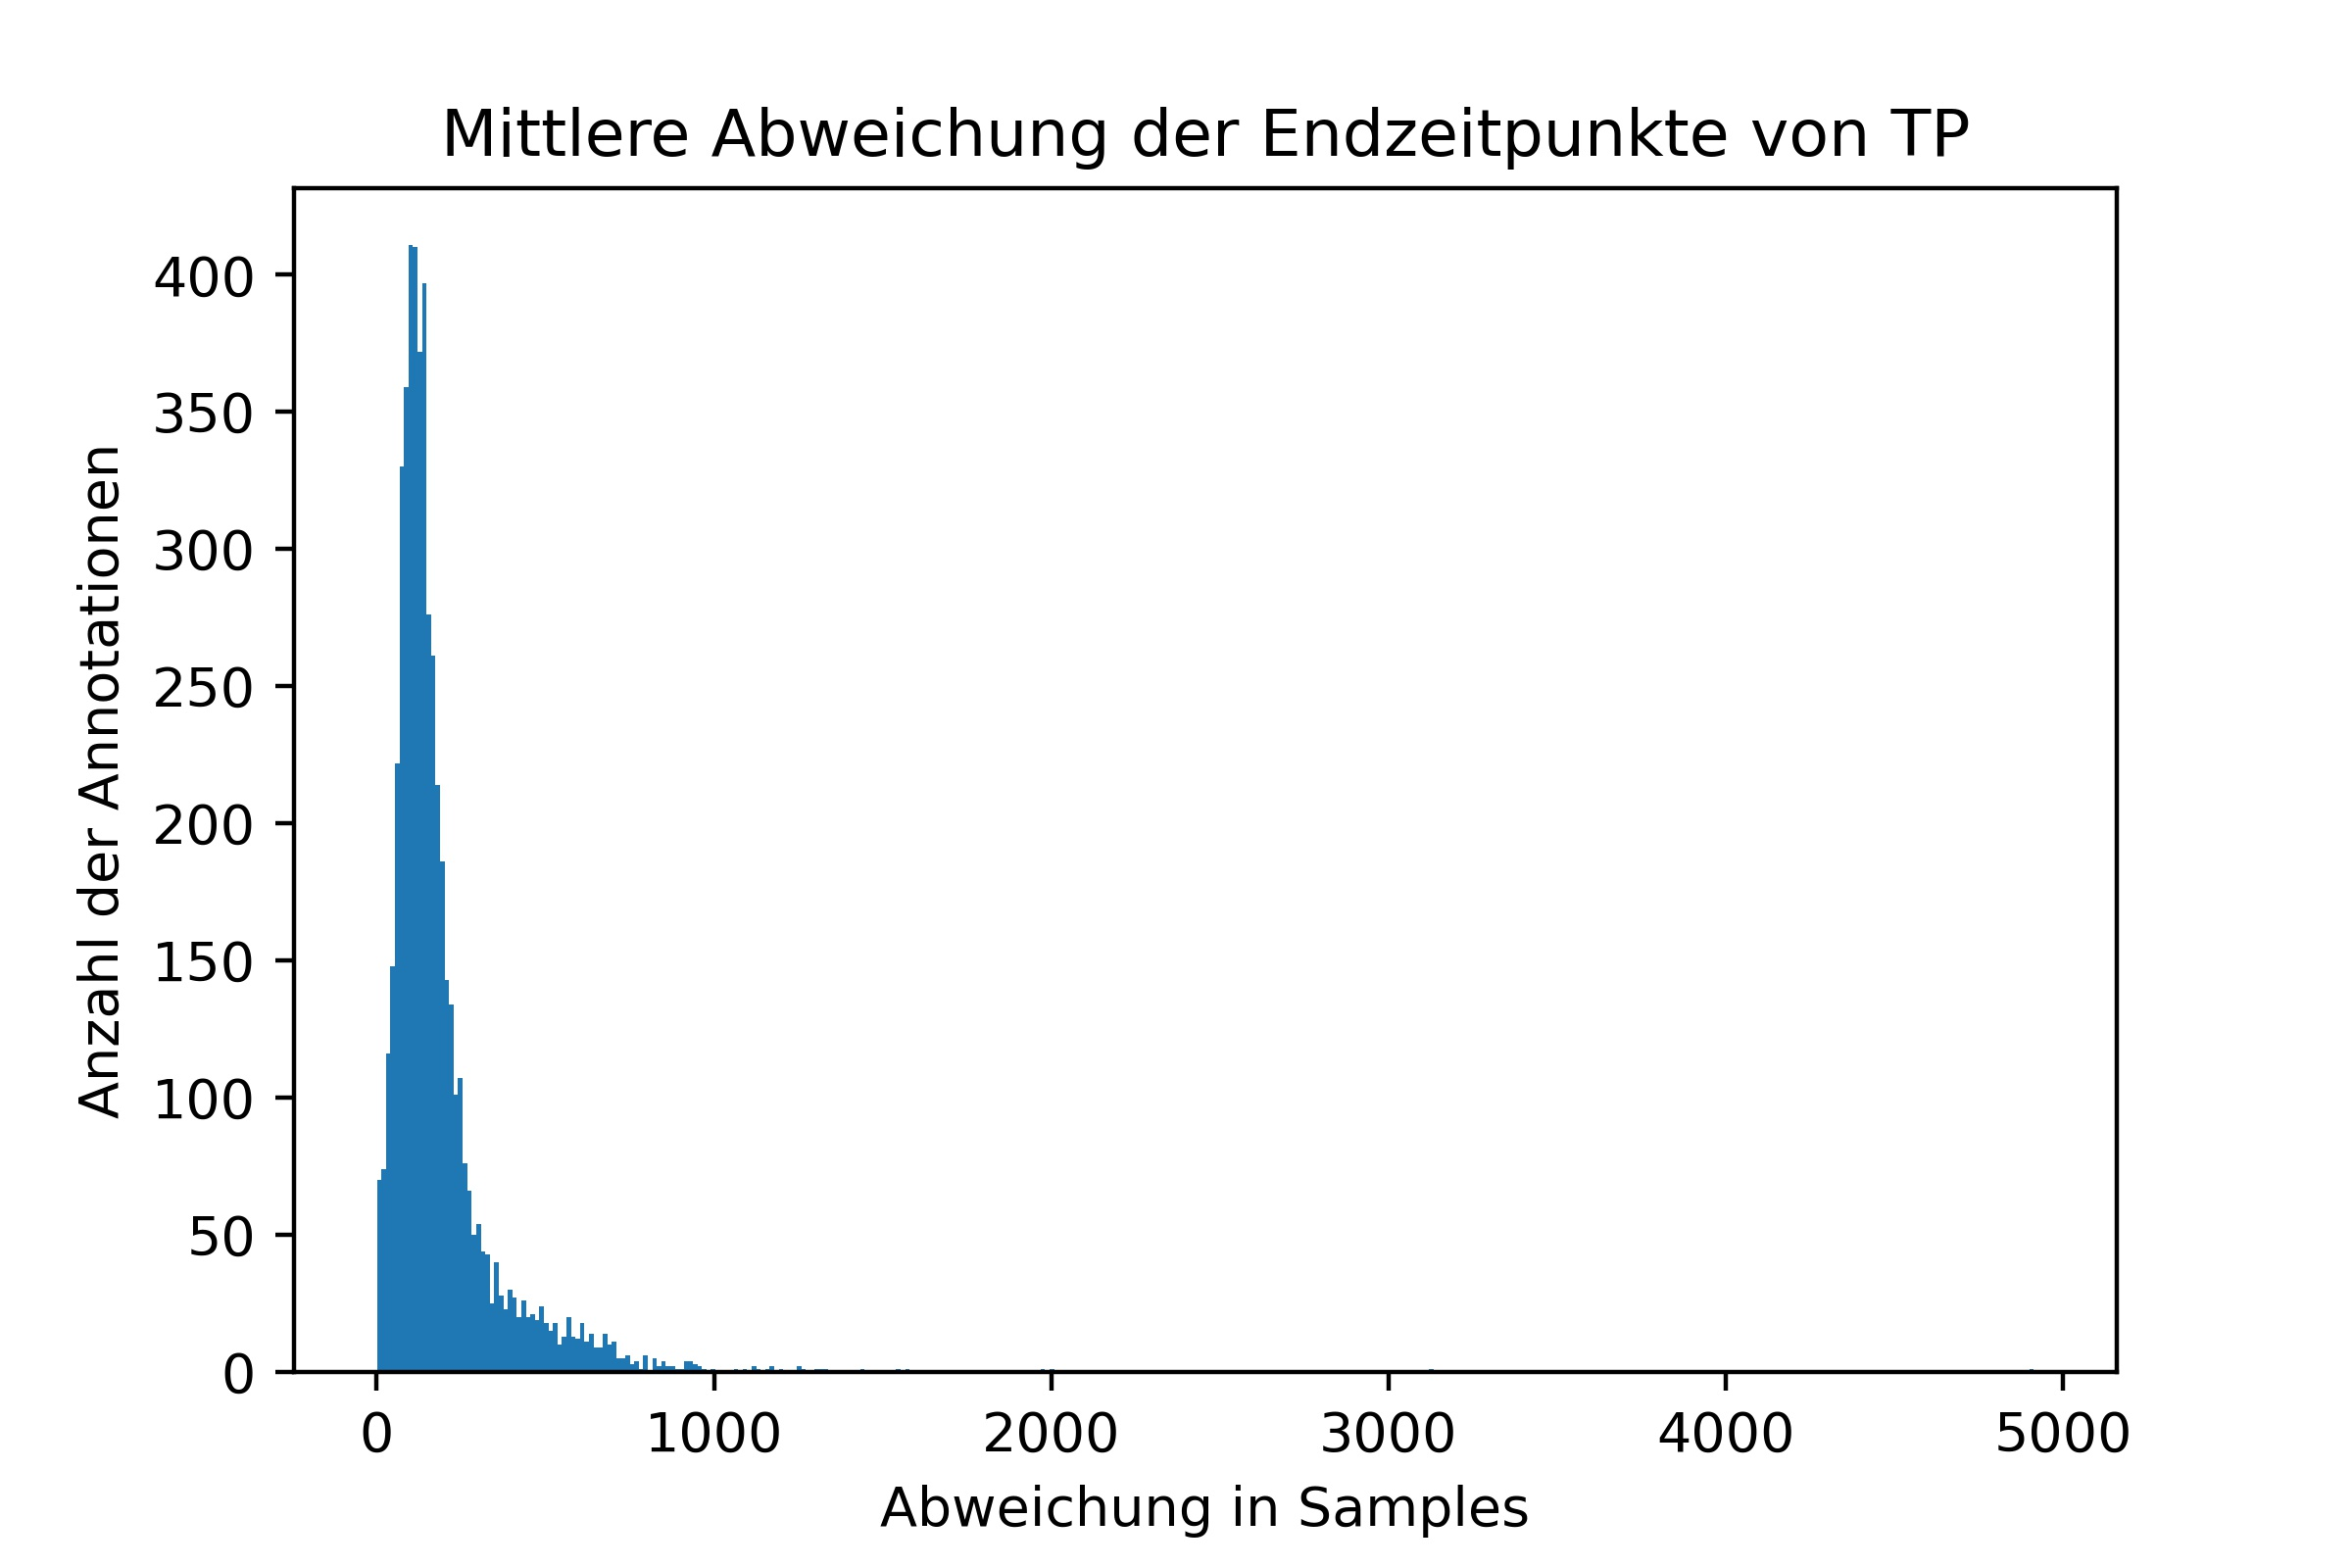
\includegraphics[width=0.80\textwidth]{./Bilder/LMEndDistribution_means.jpg}
	\end{center}
	\caption{Histogramm über die Mittlere Abweichung der Endzeitpunkte von TP bei einer Abtastfrequenz von 200 Hertz}%
	\label{fig:AASMKrit}%
\end{figure}


\begin{figure}[!ht]%
	\begin{center}
	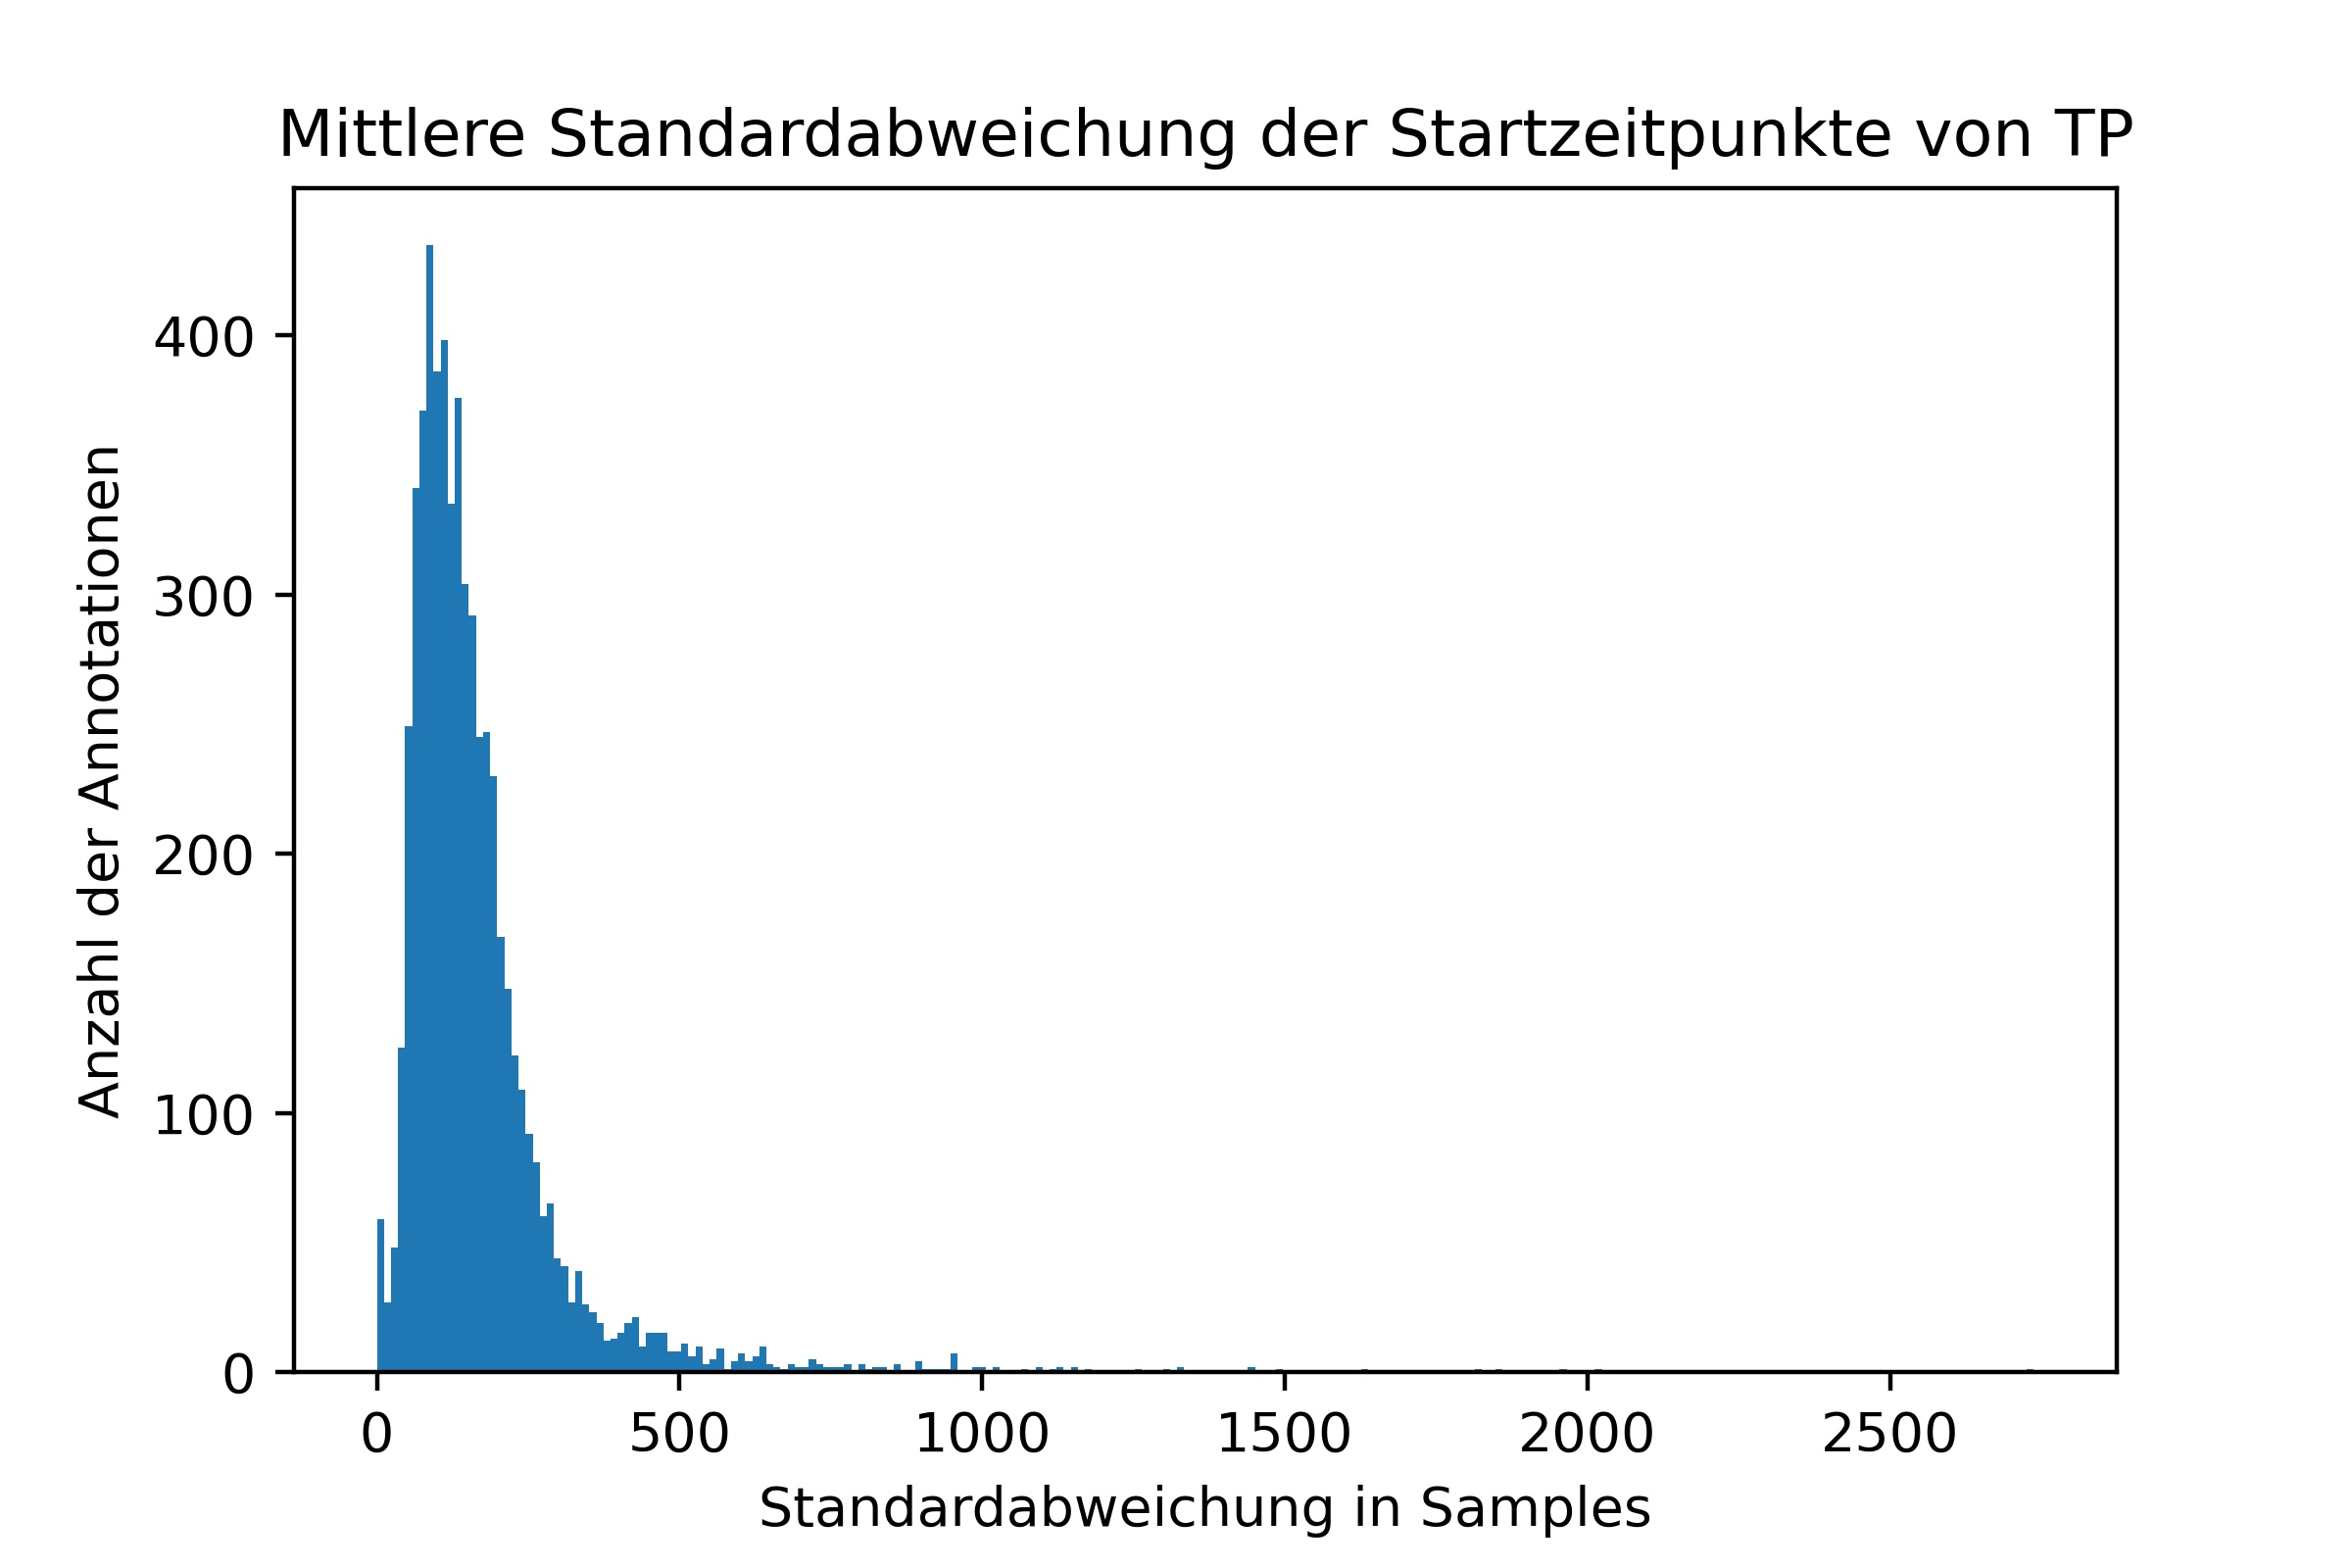
\includegraphics[width=0.80\textwidth]{./Bilder/LMStartDistribution_stds.jpg}
	\end{center}
	\caption{Histogramm über die Standardabweichung der Startzeitpunkte von TP bei einer Abtastfrequenz von 200 Hertz}%
	\label{fig:AASMKrit}%
\end{figure}

\begin{figure}[!ht]%
	\begin{center}
	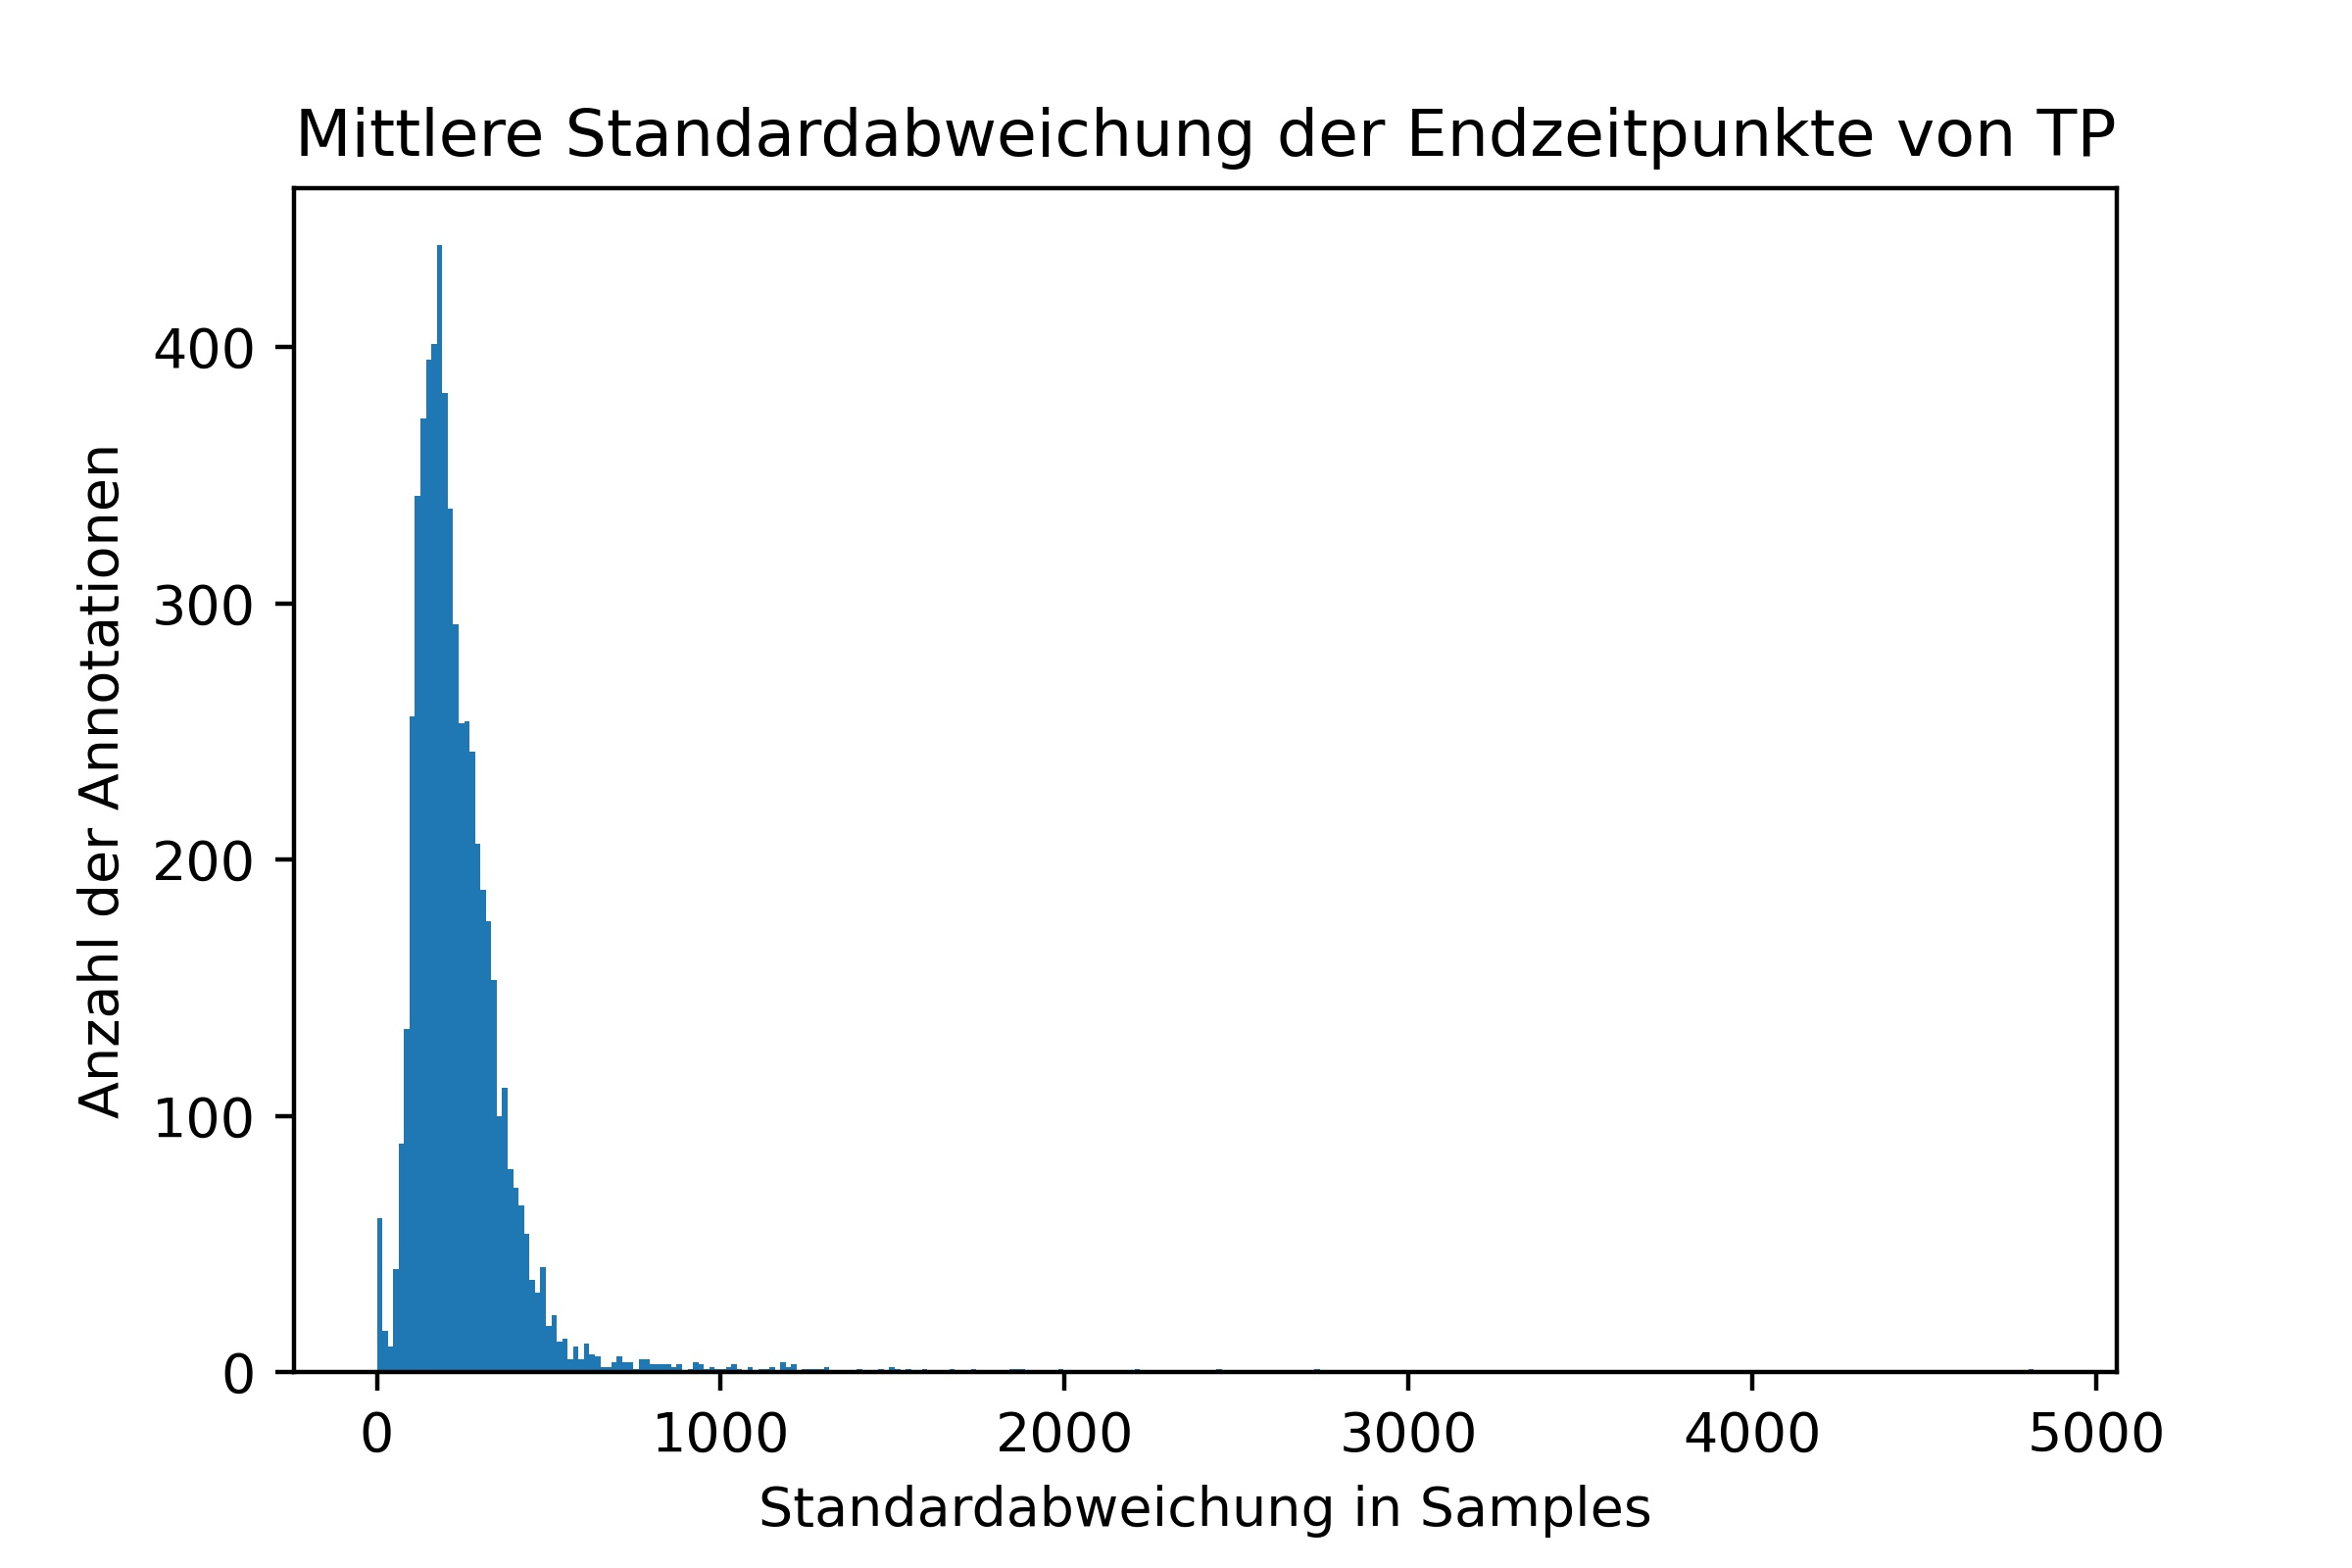
\includegraphics[width=0.80\textwidth]{./Bilder/LMEndDistribution_stds.jpg}
	\end{center}
	\caption{Histogramm über die Standardabweichung der Endzeitpunkte von TP bei einer Abtastfrequenz von 200 Hertz}%
	\label{fig:AASMKrit}%
\end{figure}

\begin{figure}[!ht]%
	\begin{center}
	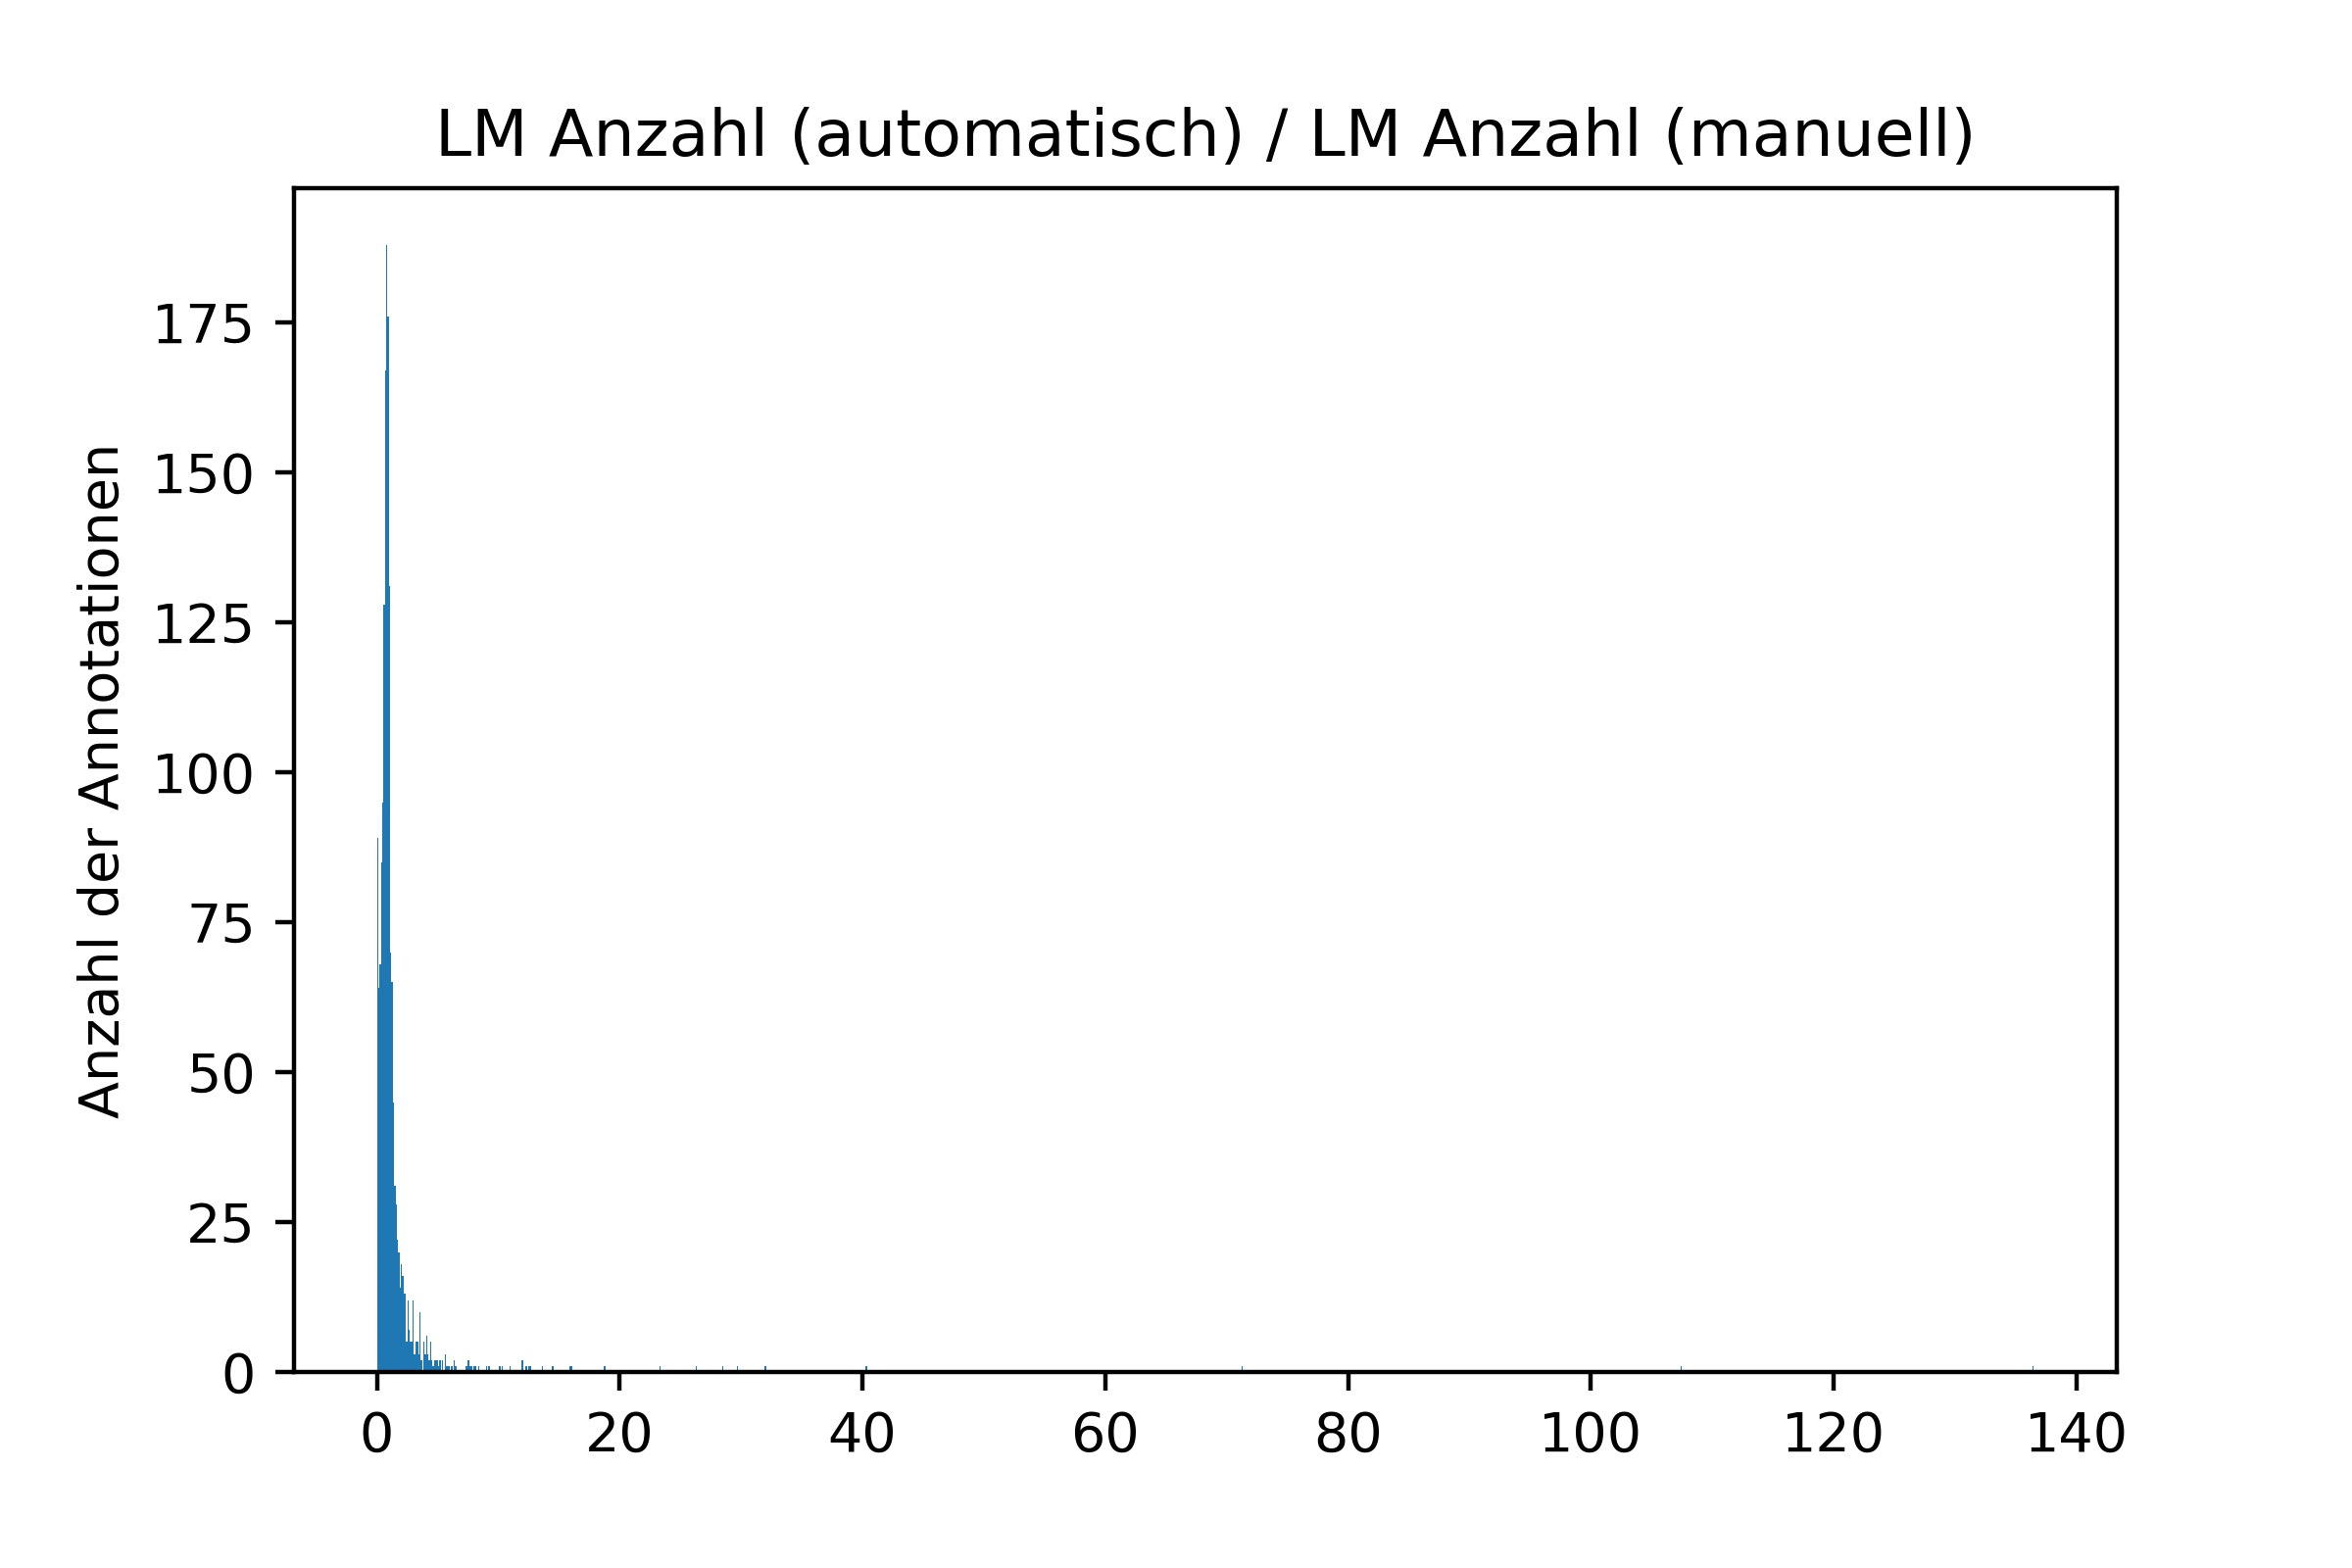
\includegraphics[width=0.80\textwidth]{./Bilder/LMcountrel.jpg}
	\end{center}
	\caption{Histogramm über das Verhältnis aus automatischer zu manueller LM Anzahl}%
	\label{fig:AASMKrit}%
\end{figure}


\begin{figure}[!ht]%
	\begin{center}
	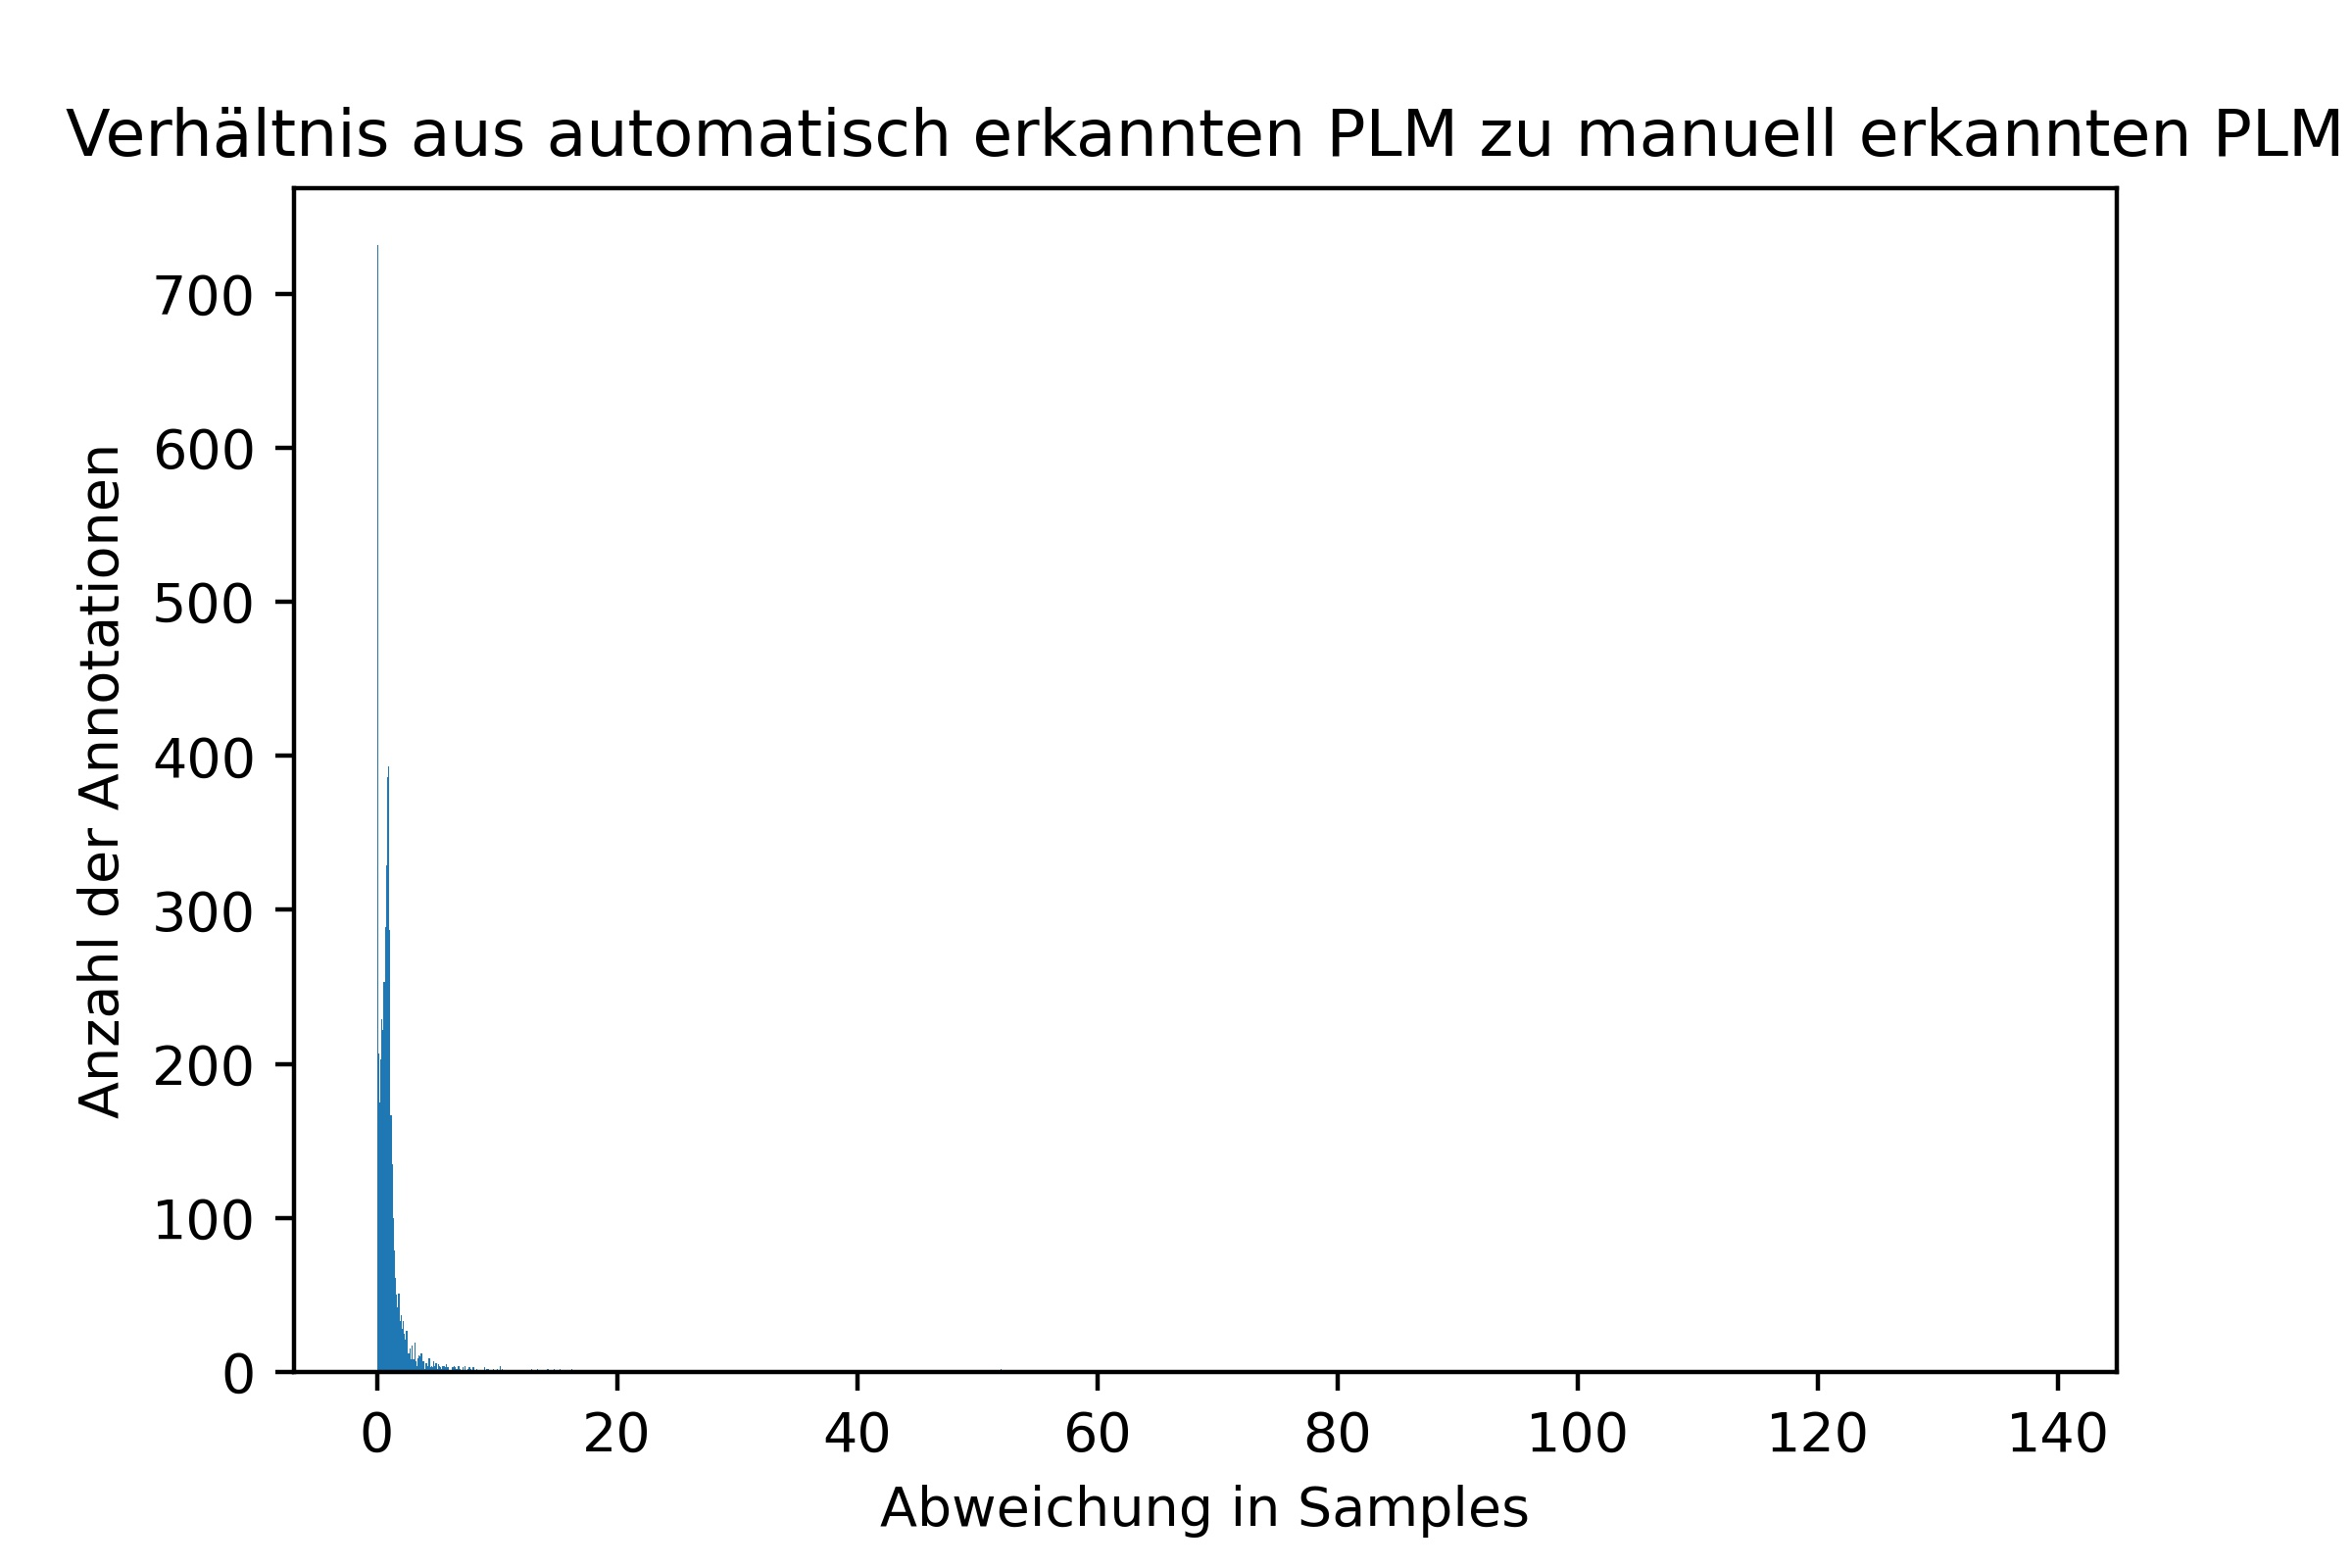
\includegraphics[width=0.80\textwidth]{./Bilder/Verhältnis aus automatisch erkannten PLM zu manuell erkannten PLM.jpg}
	\end{center}
	\caption{Histogramm über das Verhältnis aus automatischer zu manueller PLM Anzahl}%
	\label{fig:AASMKrit}%
\end{figure}



						
\end{document}